\documentclass{article}
\usepackage{mathtools,tabu,float,hyperref,color,amsmath,amsxtra,amssymb,latexsym,amscd,amsthm,amsfonts,graphicx,enumitem,multirow,datetime,listings}
\usepackage[a4paper,left=3cm,right=3cm,top=3cm,bottom=3cm]{geometry}
\usepackage{tikz,graphicx}
\usetikzlibrary{shapes,arrows}
\usetikzlibrary{calc}
\usetikzlibrary{decorations.pathmorphing}
\usepackage{caption}
\usepackage[english]{babel}
\begin{document}
	\title{User Guide for Code to solve systems of ODEs using Runge-Kutta method\\On systems running Microsoft Windows 10}
	\maketitle
	\begin{abstract}
		This is only the guide to use our code for the purpose said in the title, for more theoretical details, please see \cite{1} and \cite{2}. For reference to the \texttt{Fortran} programming language, you may want to visit \cite{3}.
	\end{abstract}
	\tableofcontents
	\newpage
	\noindent
	\section{Preparation}
	To use our code, which was written in \texttt{Fortran}, we need the following things on a system running Windows 10:
	\begin{enumerate}
		\item A text editor: You can use any text editor, but in this guide, we will use \texttt{gedit}, you can download it at \url{https://wiki.gnome.org/Apps/Gedit#Download}.
		\item \texttt{gfortran}: You can download an unofficial build of GCC 5 source at \url{https://gcc.gnu.org/wiki/GFortranBinaries#Windows}, or more explicitly, \url{http://users.humboldt.edu/finneyb/gfortran-windows-20140629.exe}
		\item \texttt{gnuplot}: You can download it at \texttt{gnuplot} primary download site on SourceForge: \url{https://sourceforge.net/projects/gnuplot/files/gnuplot/}
	\end{enumerate}
	\noindent$\bullet$ \textbf{Important note:} When installing \texttt{gnuplot}, you must tick the option "Add application directory to your PATH environment variable".
	\begin{figure}[H]
		\centering	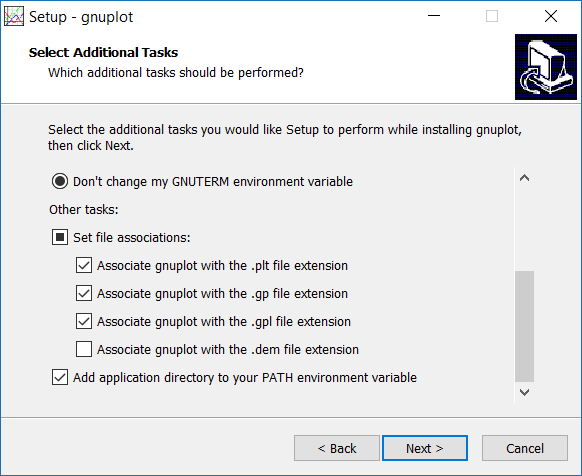
\includegraphics[width=15cm]{figextra1}
		\caption{Tick the option "Add application directory to your PATH environment variable"}
	\end{figure}
	\noindent$\bullet$ \textbf{However, if you miss that option}, you can add the \texttt{gnuplot} directory to the PATH environment variable manually by the following steps. Otherwise, you may skip to \autoref{section2}.
	\begin{figure}[H]
		\centering	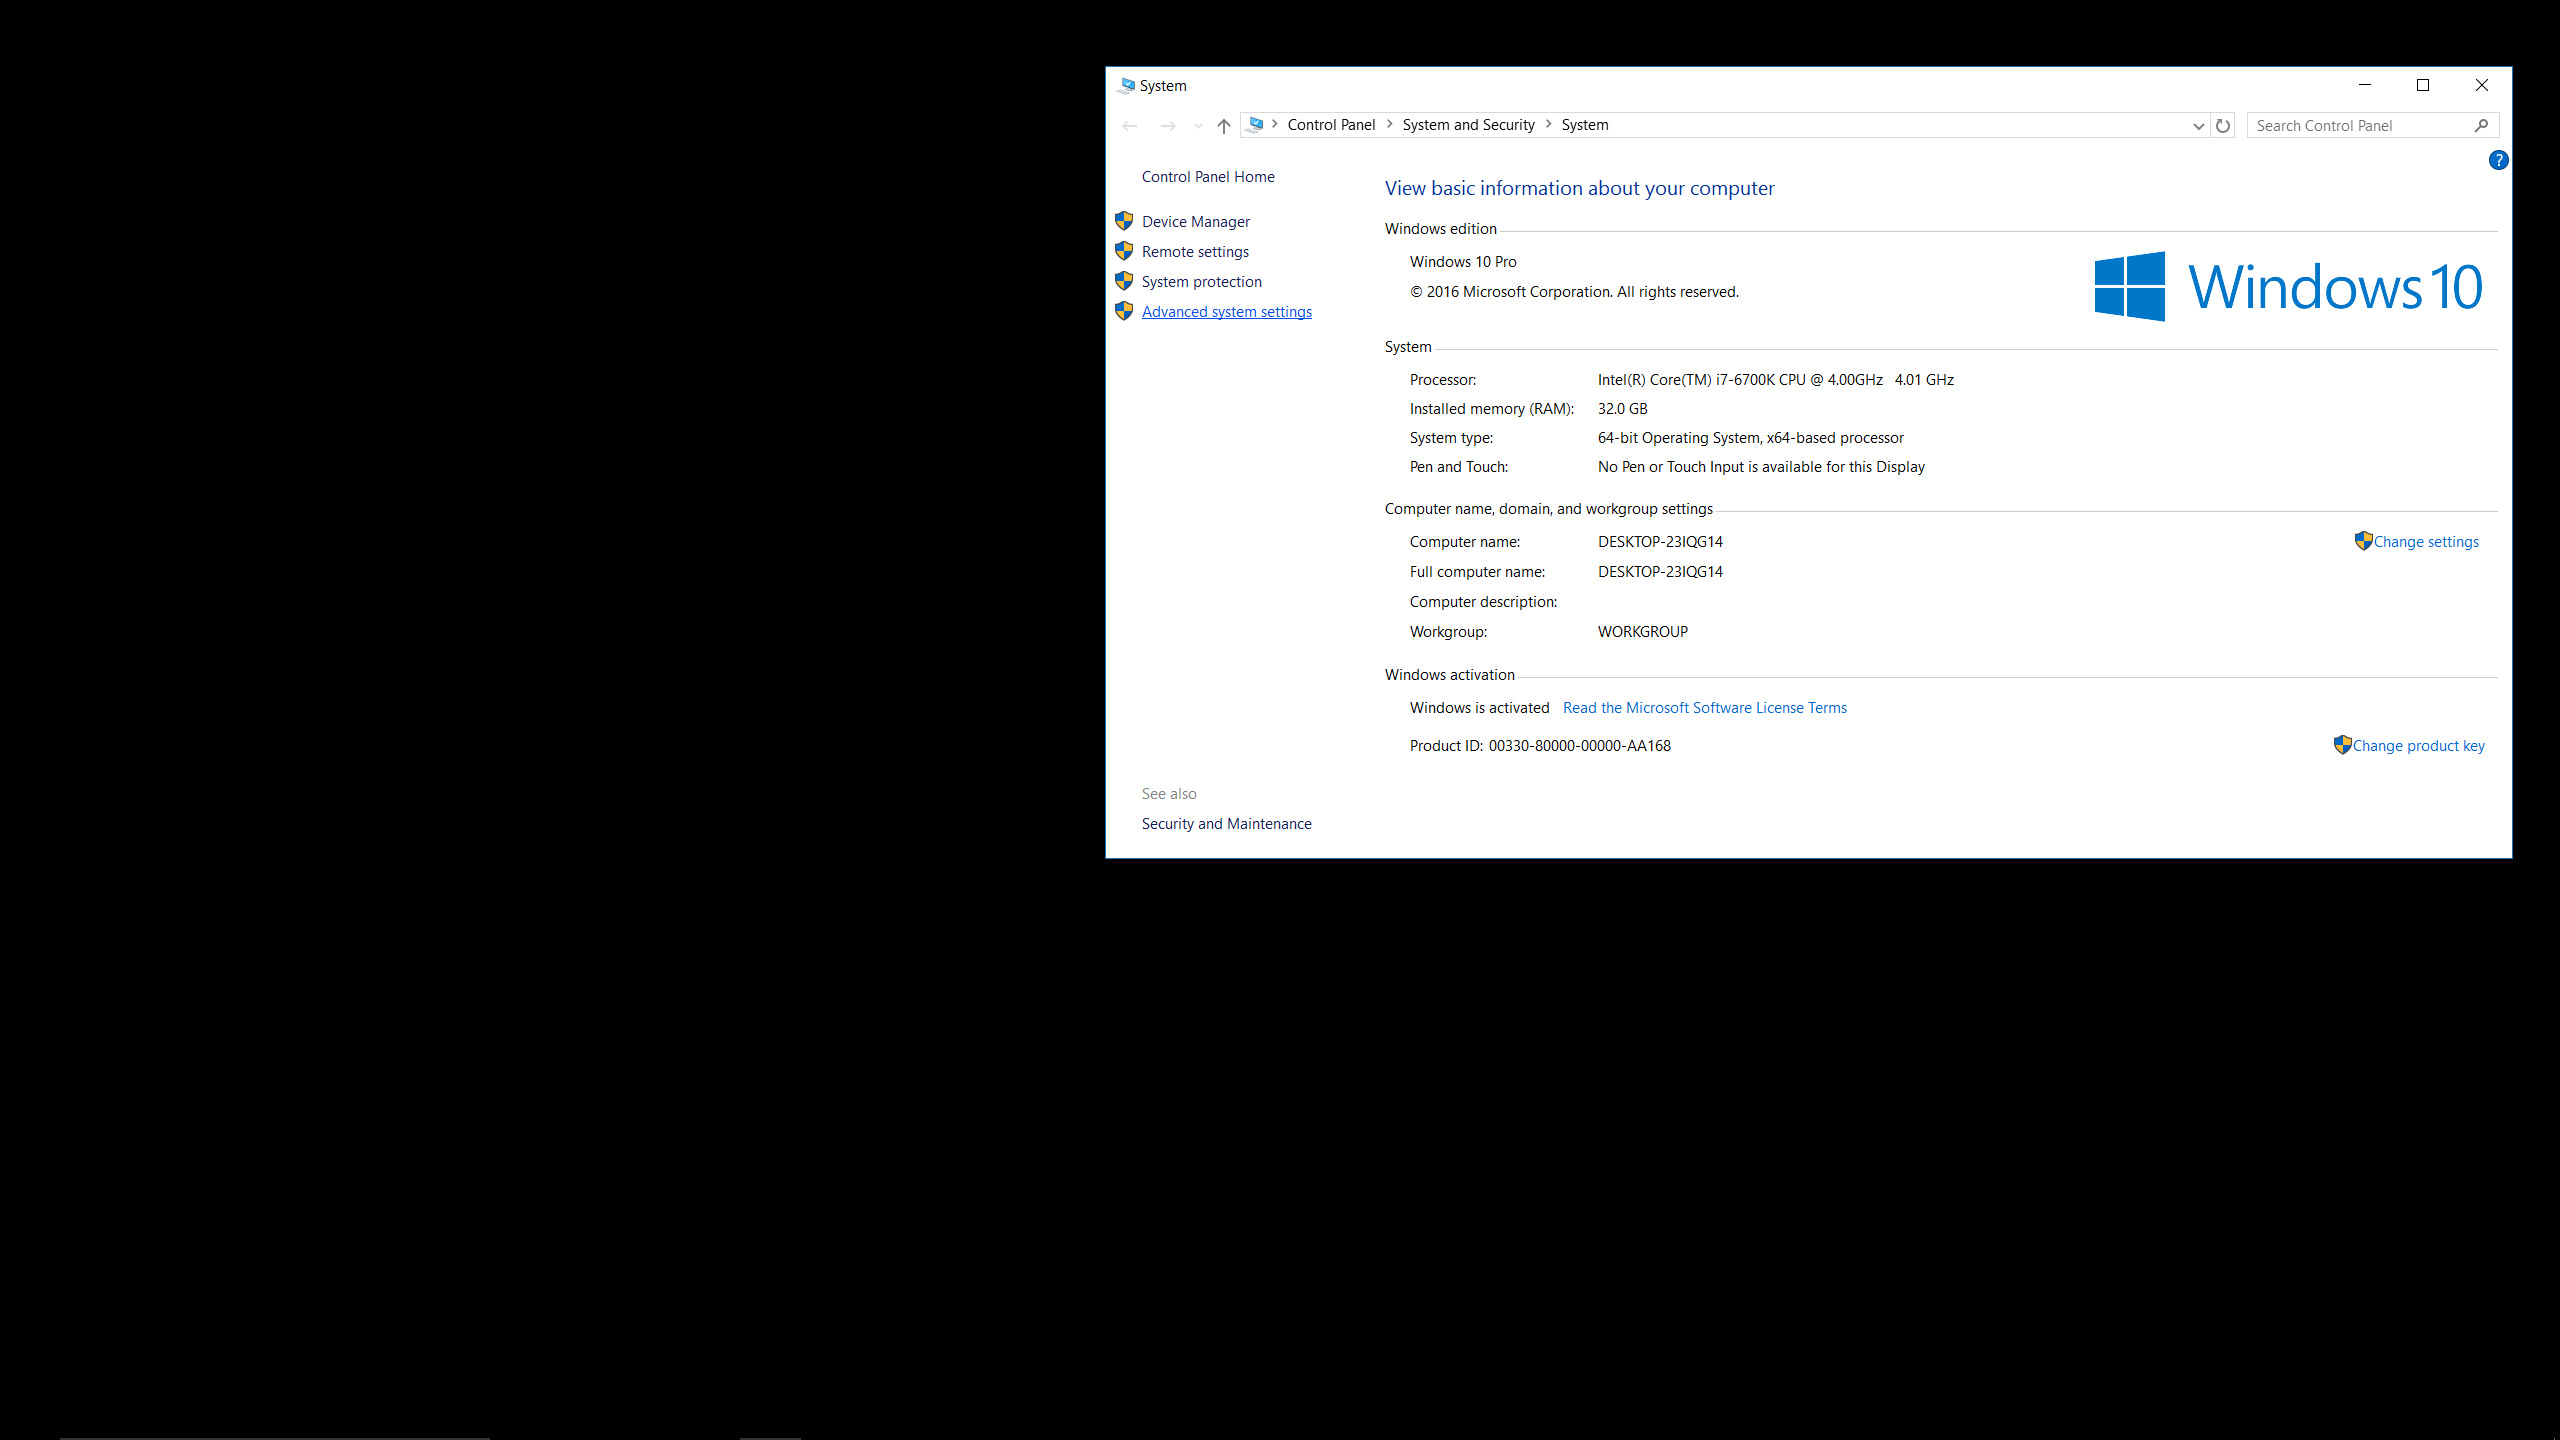
\includegraphics[width=15cm]{figextra2}
		\caption{Press \textbf{Windows key + Pa/Br} to open system properties window}
	\end{figure}
	\begin{figure}[H]
		\centering	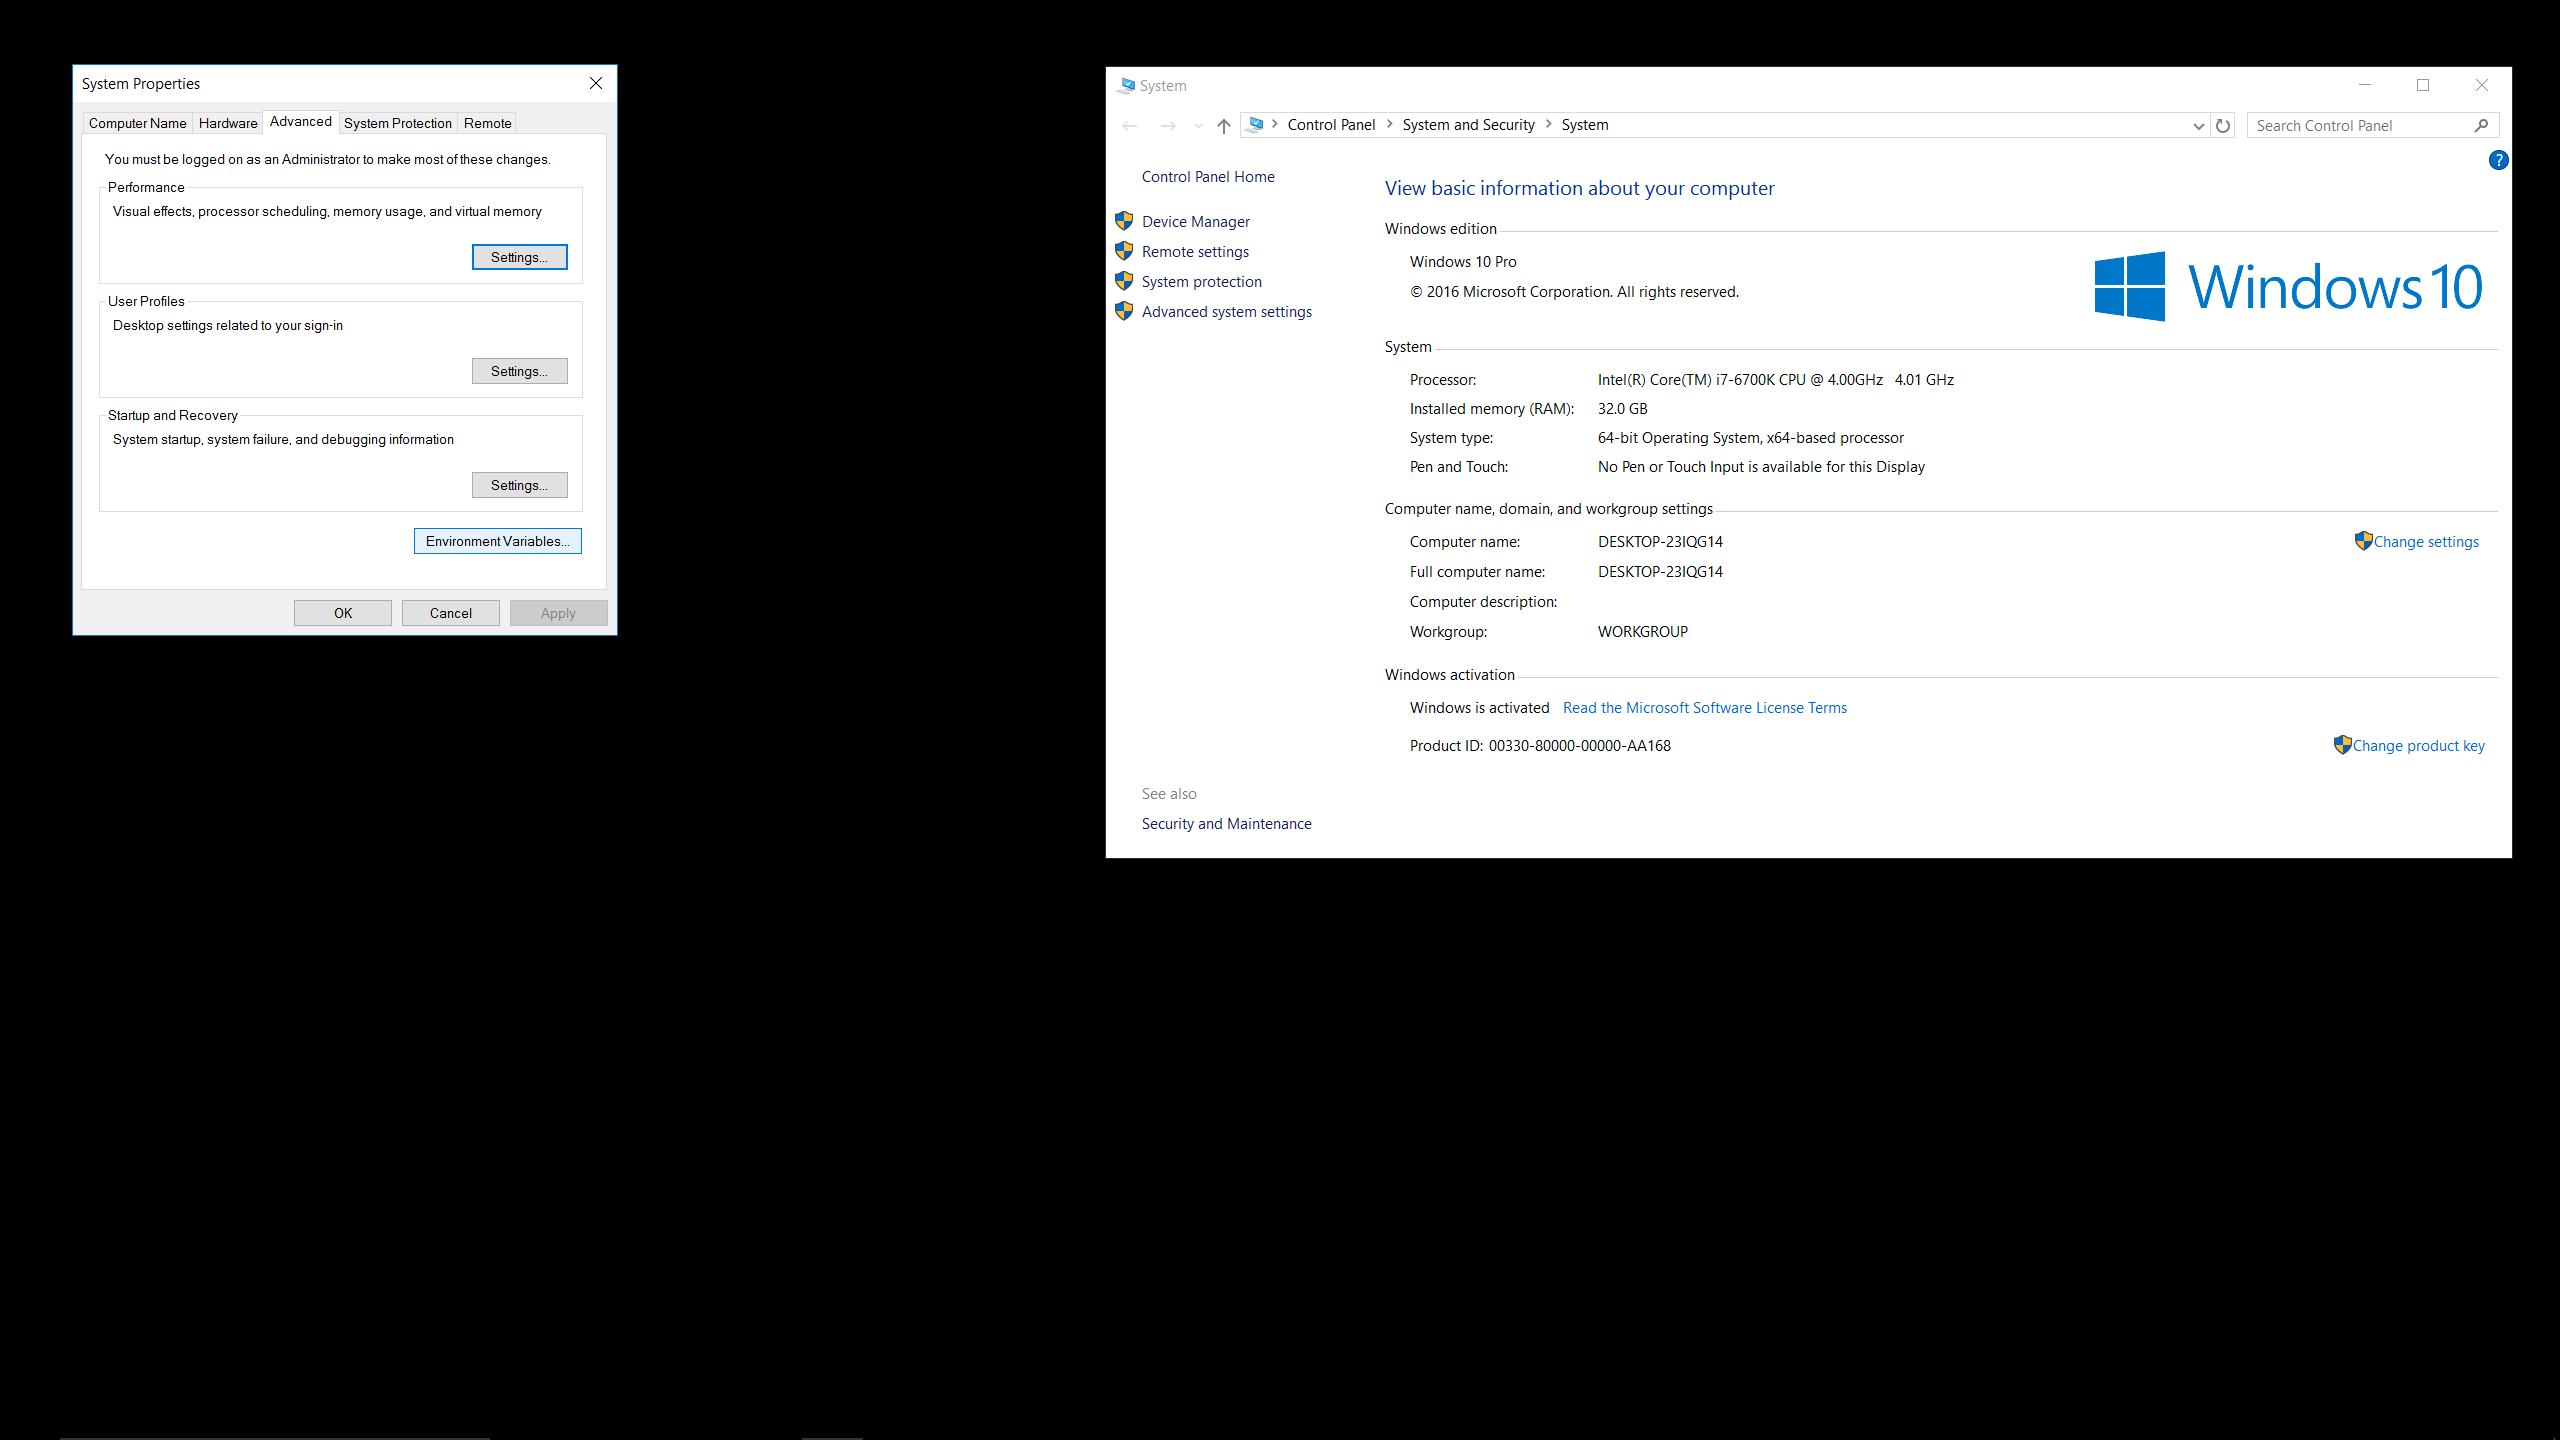
\includegraphics[width=15cm]{figextra3}
		\caption{Click on \textbf{Advanced system settings} on the left side to open "Advanced" tab in "System properties"}
	\end{figure}
	\begin{figure}[H]
		\centering	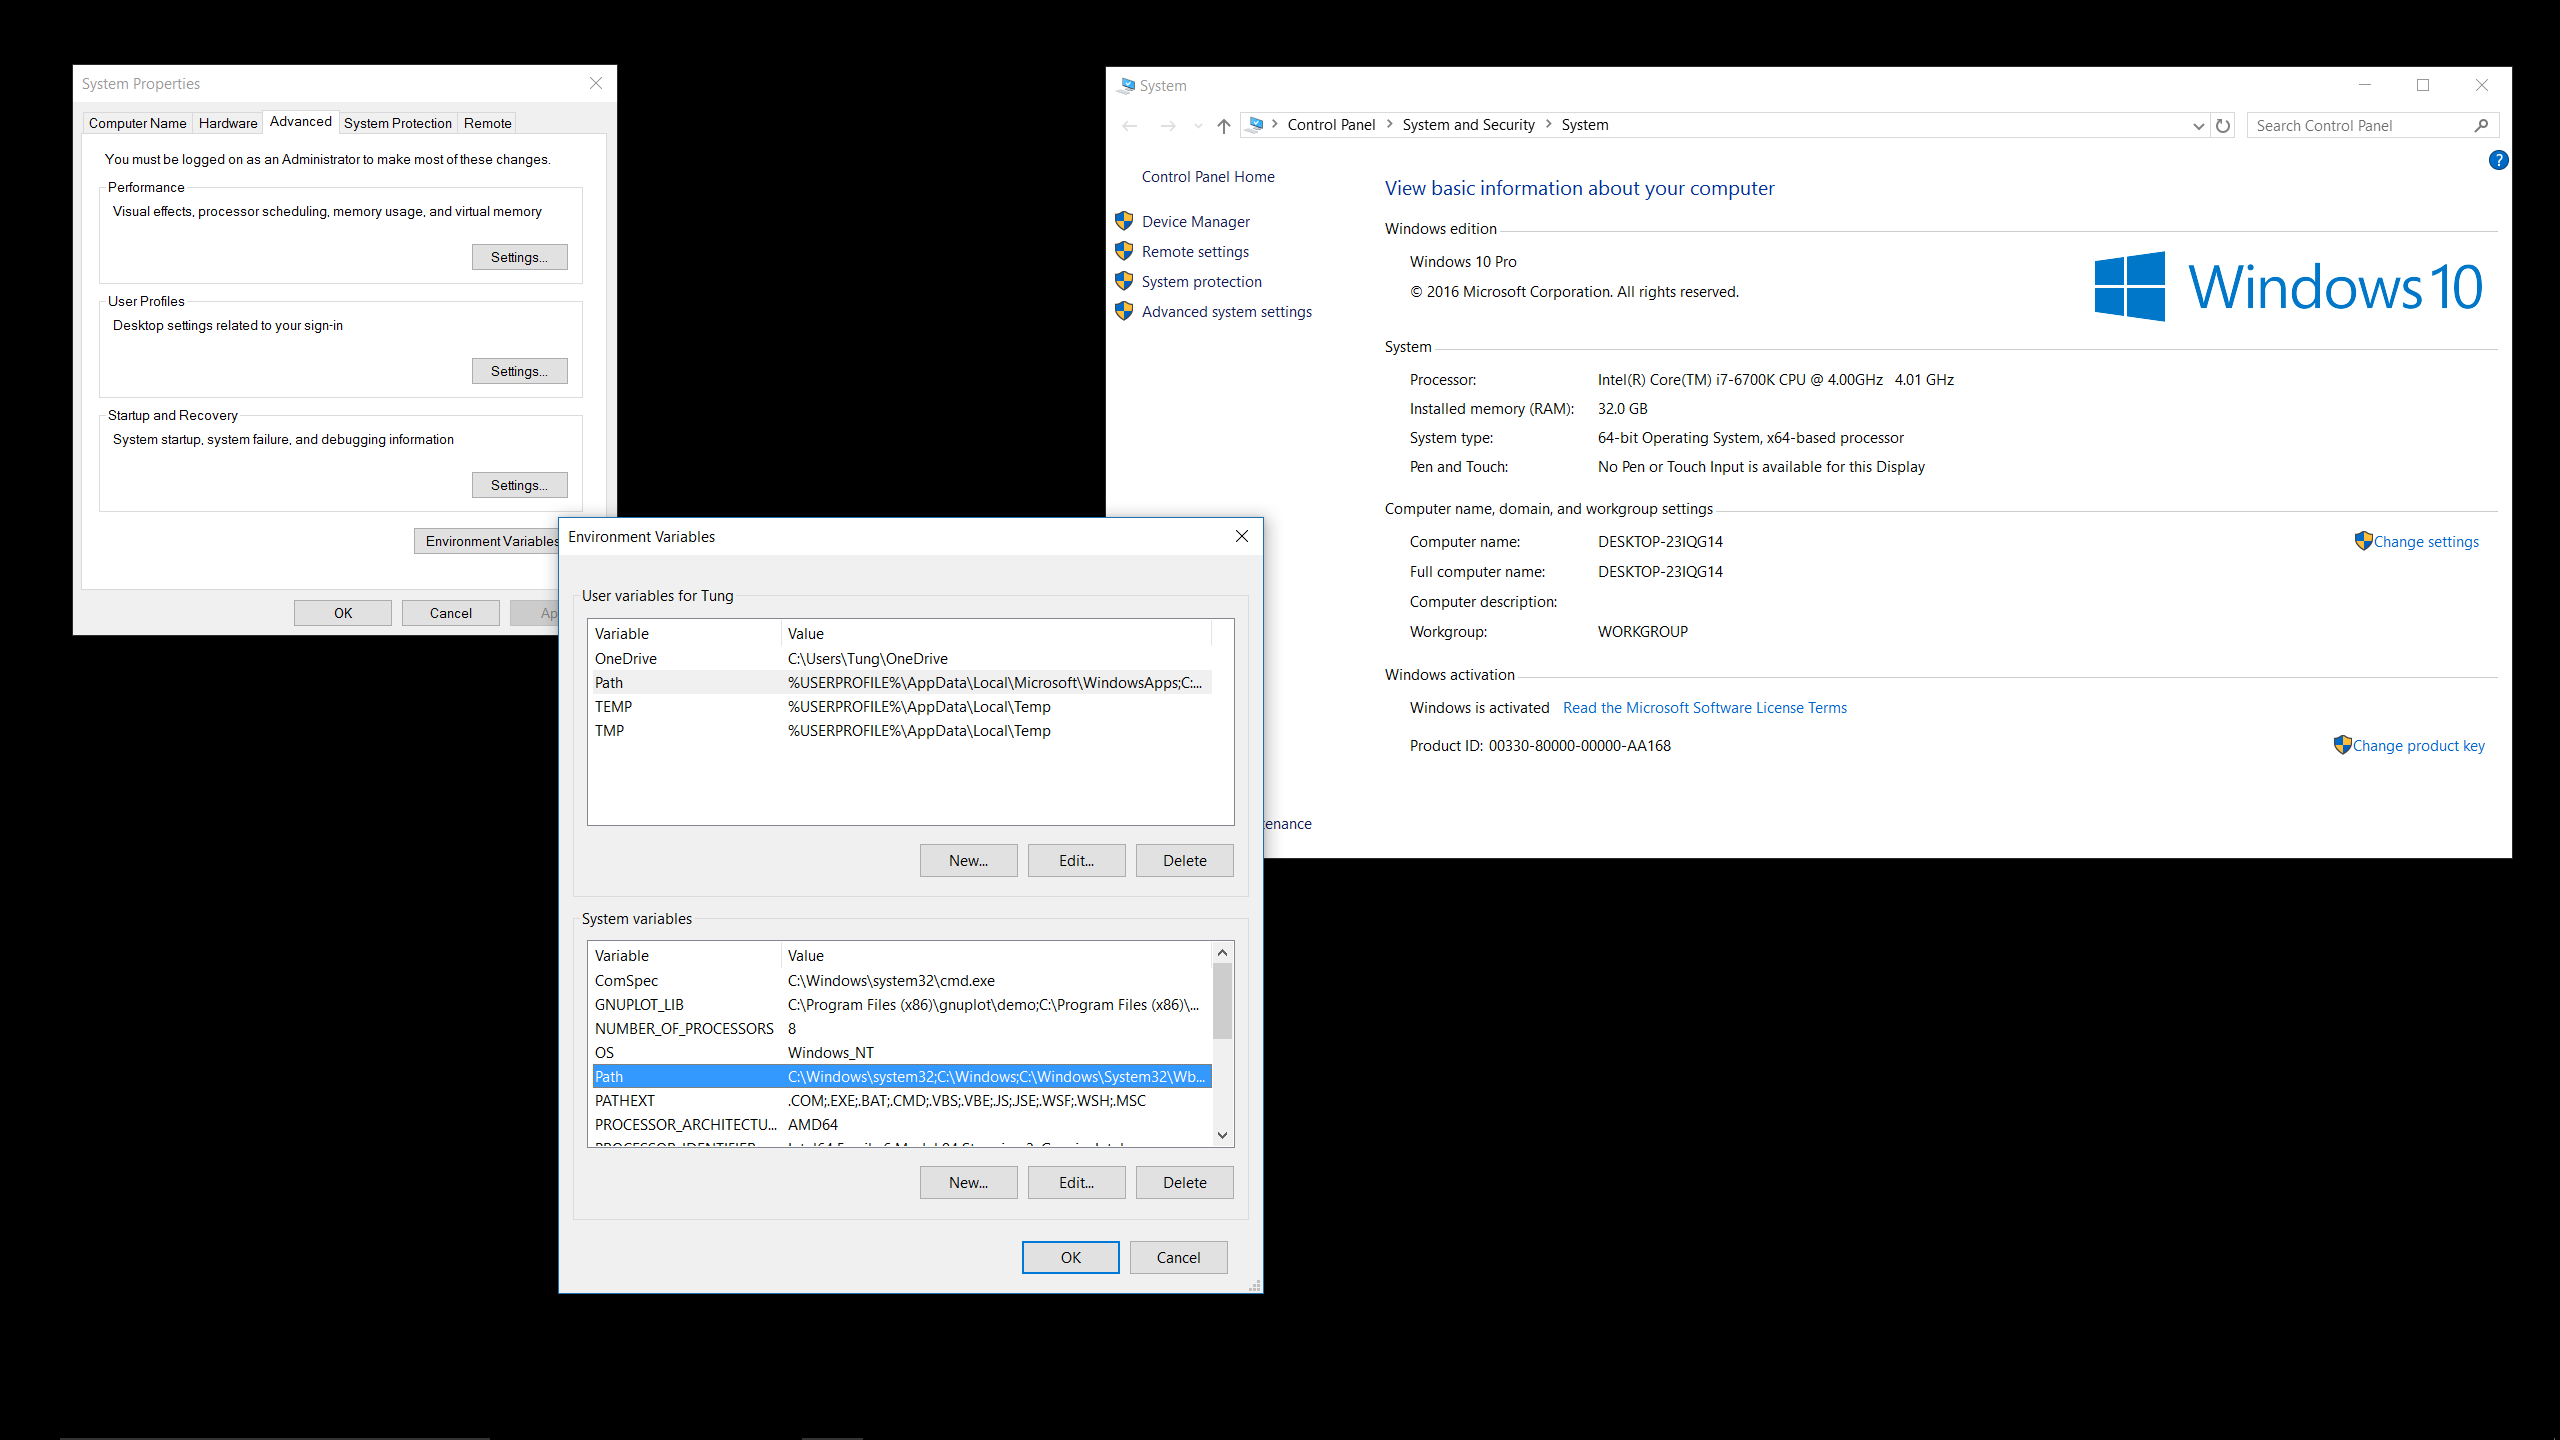
\includegraphics[width=15cm]{figextra4}
		\caption{Click on \textbf{Environment Variables} to open "Environment Variables" window and highlight the \textbf{Path} variable in the "System variable" section}
	\end{figure}
	\begin{figure}[H]
		\centering	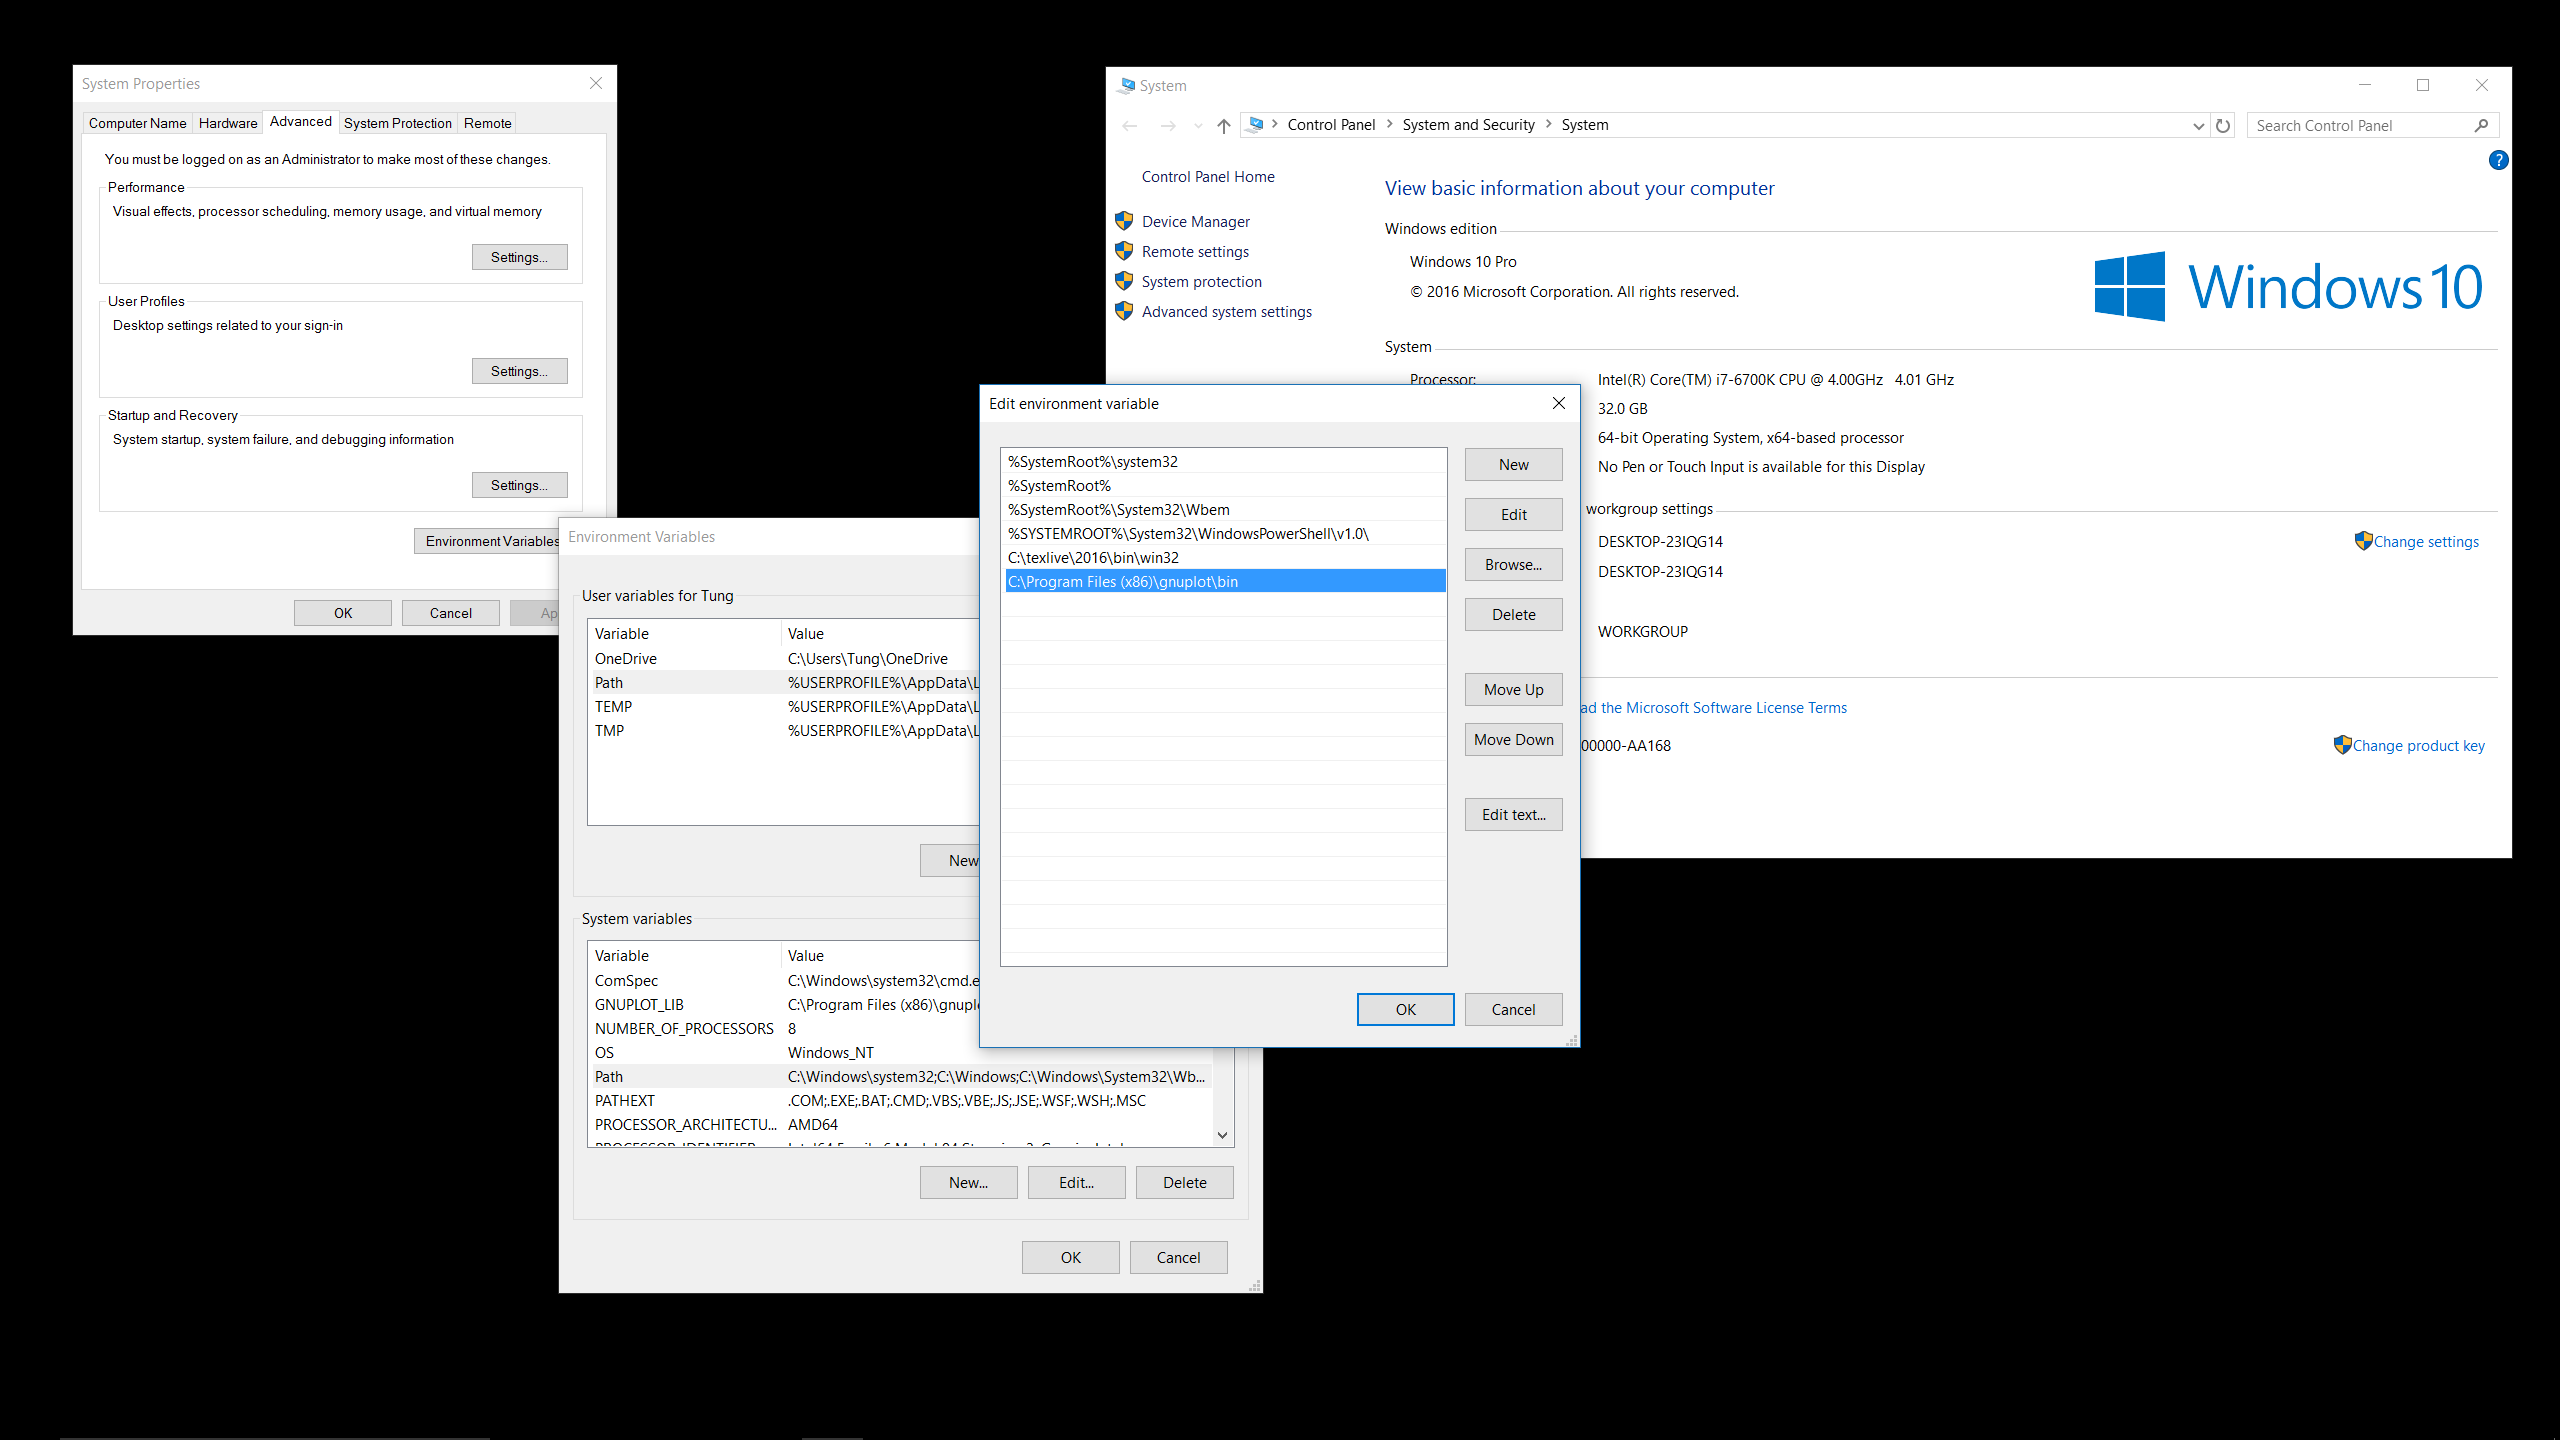
\includegraphics[width=15cm]{figextra5}
		\caption{Click the \textbf{Edit} button to open "Edit environment variable" window and add the \texttt{gnuplot} directory there}
	\end{figure}
	\section{The source files}\label{section2}
	We wrote multiple source files with different purposes:
	\begin{itemize}
		\item \texttt{rkfts.f90}: \texttt{Fortran} source code for Runge-Kutta method using fixed time step
		\item \texttt{rkats.f90}: \texttt{Fortran} source code for Runge-Kutta method using adaptive time step
		\item \texttt{data\_plot.plt} and \texttt{data\_plot\_dependency.plt} :\texttt{gnuplot} commands to plot the results
		\item \texttt{customf.f90}: source code for module containing the specific equation you want to solve, how to modify it will be discussed later.
		\item The other \texttt{*.f90}: \texttt{Fortran} source code for modules containing the example equations to solve, we included modules for: Curtiss-Hirschfelder equation, Brusselator equation, Van der Pol equation,$\dots$
	\end{itemize}
	\section{Specifying equation by modifying the source files}
	As mentioned before, there are module files containing the example equations, you may want to take a look at those and \cite{3} for reference. This section will explain about what you need to specify in the module file. For example, a module file look like this
	\begin{figure}[H]
		\centering	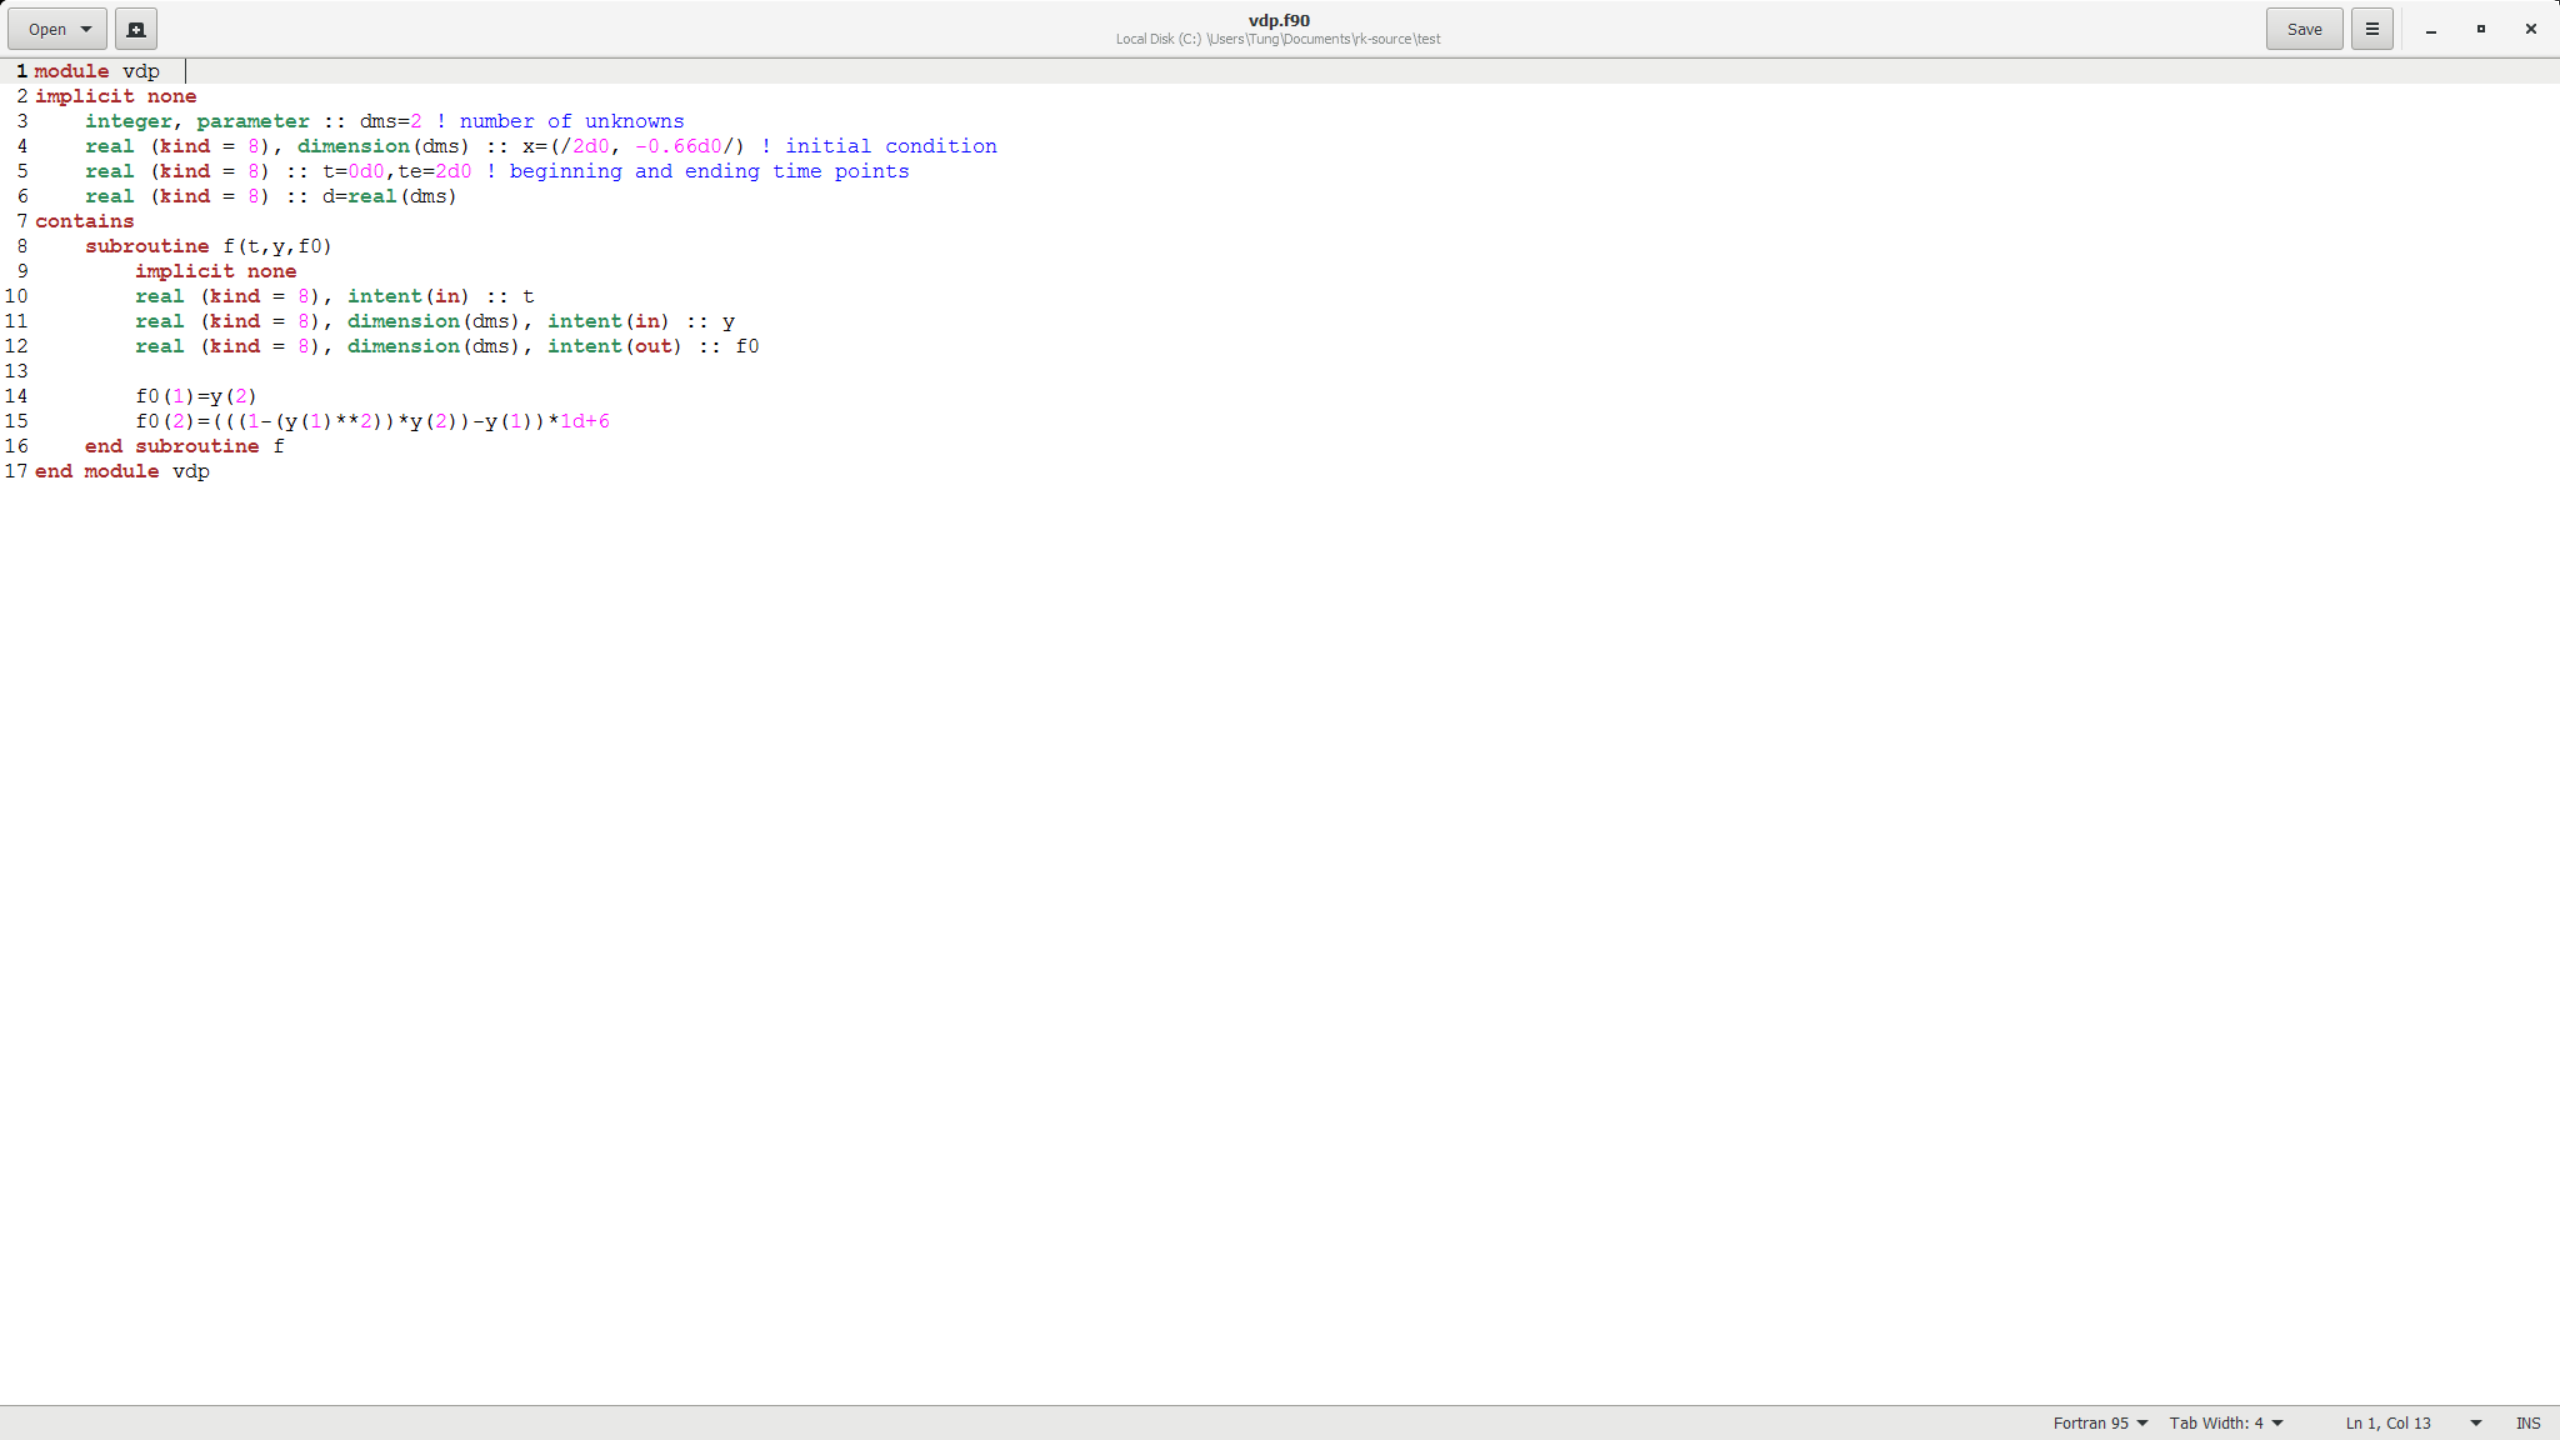
\includegraphics[width=15cm]{fig0}
		\caption{Module file of the Van der Pol equation}
		\label{module}
	\end{figure}
	\noindent As commented in the file, line $3$, $4$, $4$ contain the information about "number of unknowns", "initial conditions", "beginning and ending time points". The information in \autoref{module} means that we are considering a equation with $2$ unknown variables, the beginning and ending time points are $t_0=0$ and $t_e=2$ respectively, the initial condition is $f(0,y)=(2,-0.66)$.\\
	Where $y=y_1,y_2$ is the vector of unknown variables and 
	\begin{flalign*}
		f(t,y)=\left[y_2(t) , \dfrac{\left(1-y_1(t)\right)^2y_2(t)-y_1(t)}{10^{-6}}\right]
	\end{flalign*}
	\noindent More ever, we may also need to modify the time step in \texttt{rkfts.f90} or the error tolerance in \texttt{rkats.f90}, for more details about this, refer to \cite{1} and \cite{2}.
	\begin{figure}[H]
		\centering	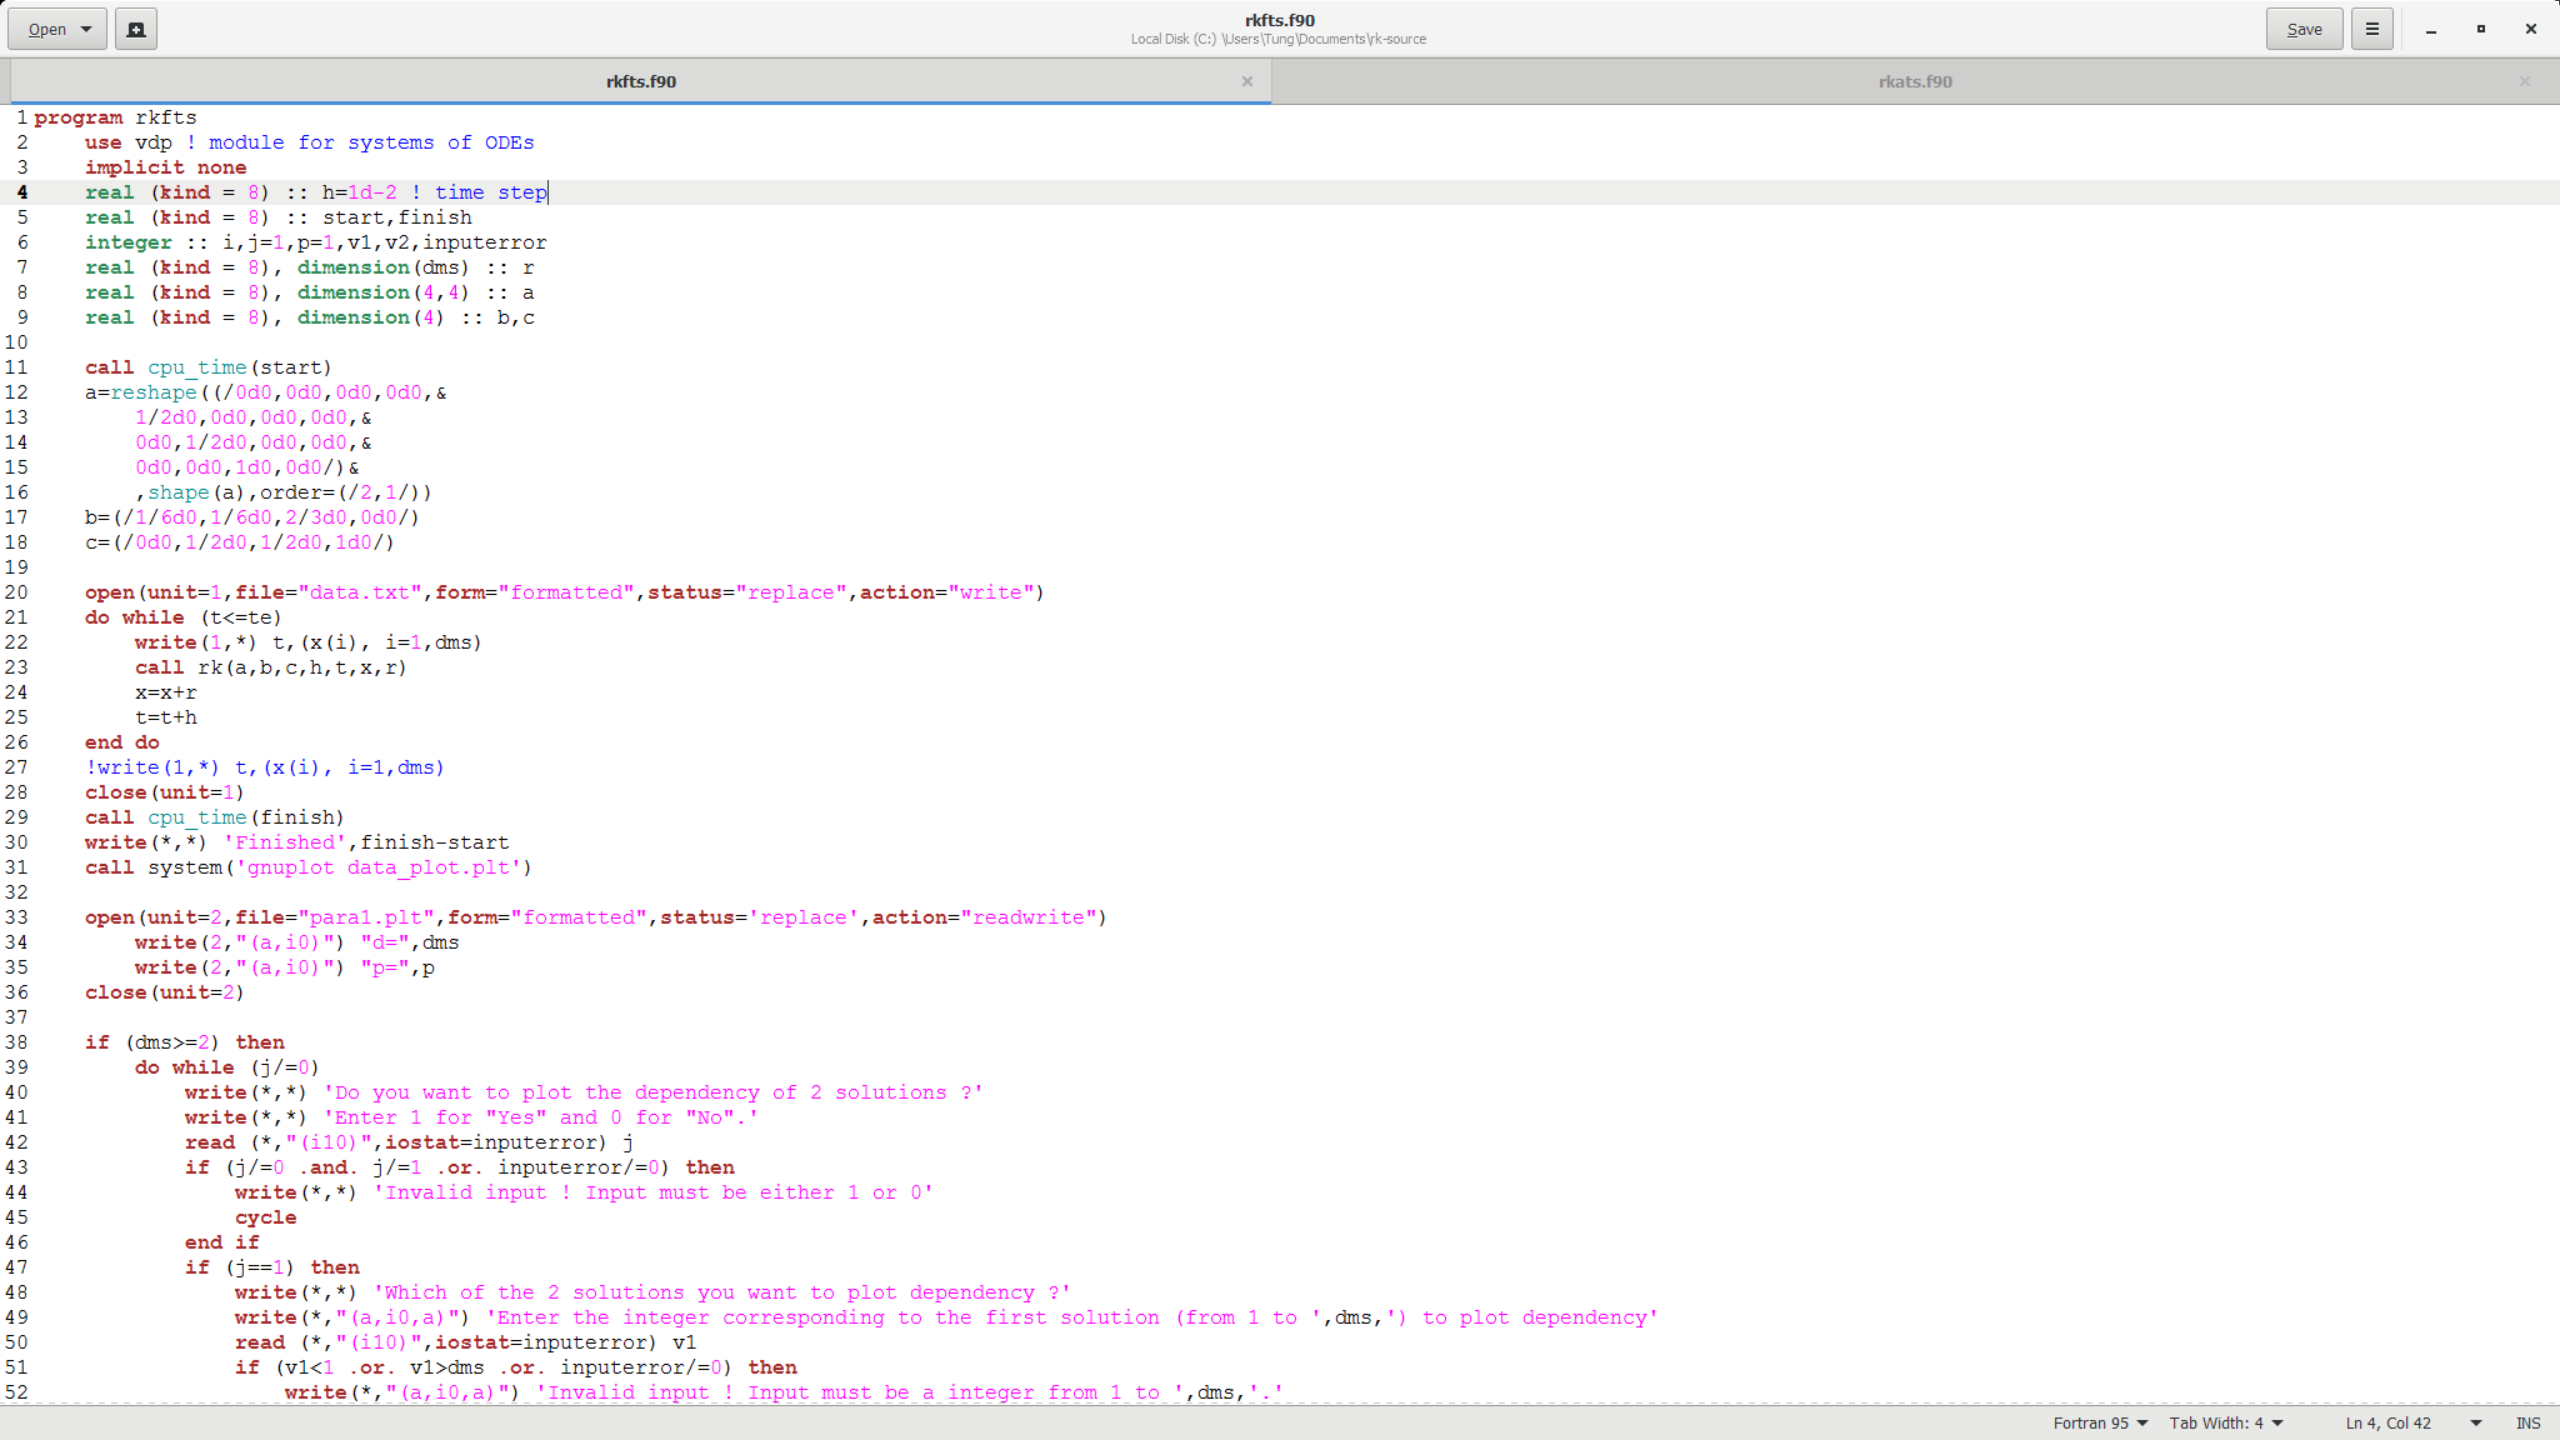
\includegraphics[width=15cm]{fig01}
		\caption{rkfts.f90}
	\end{figure}
	\begin{figure}[H]
		\centering	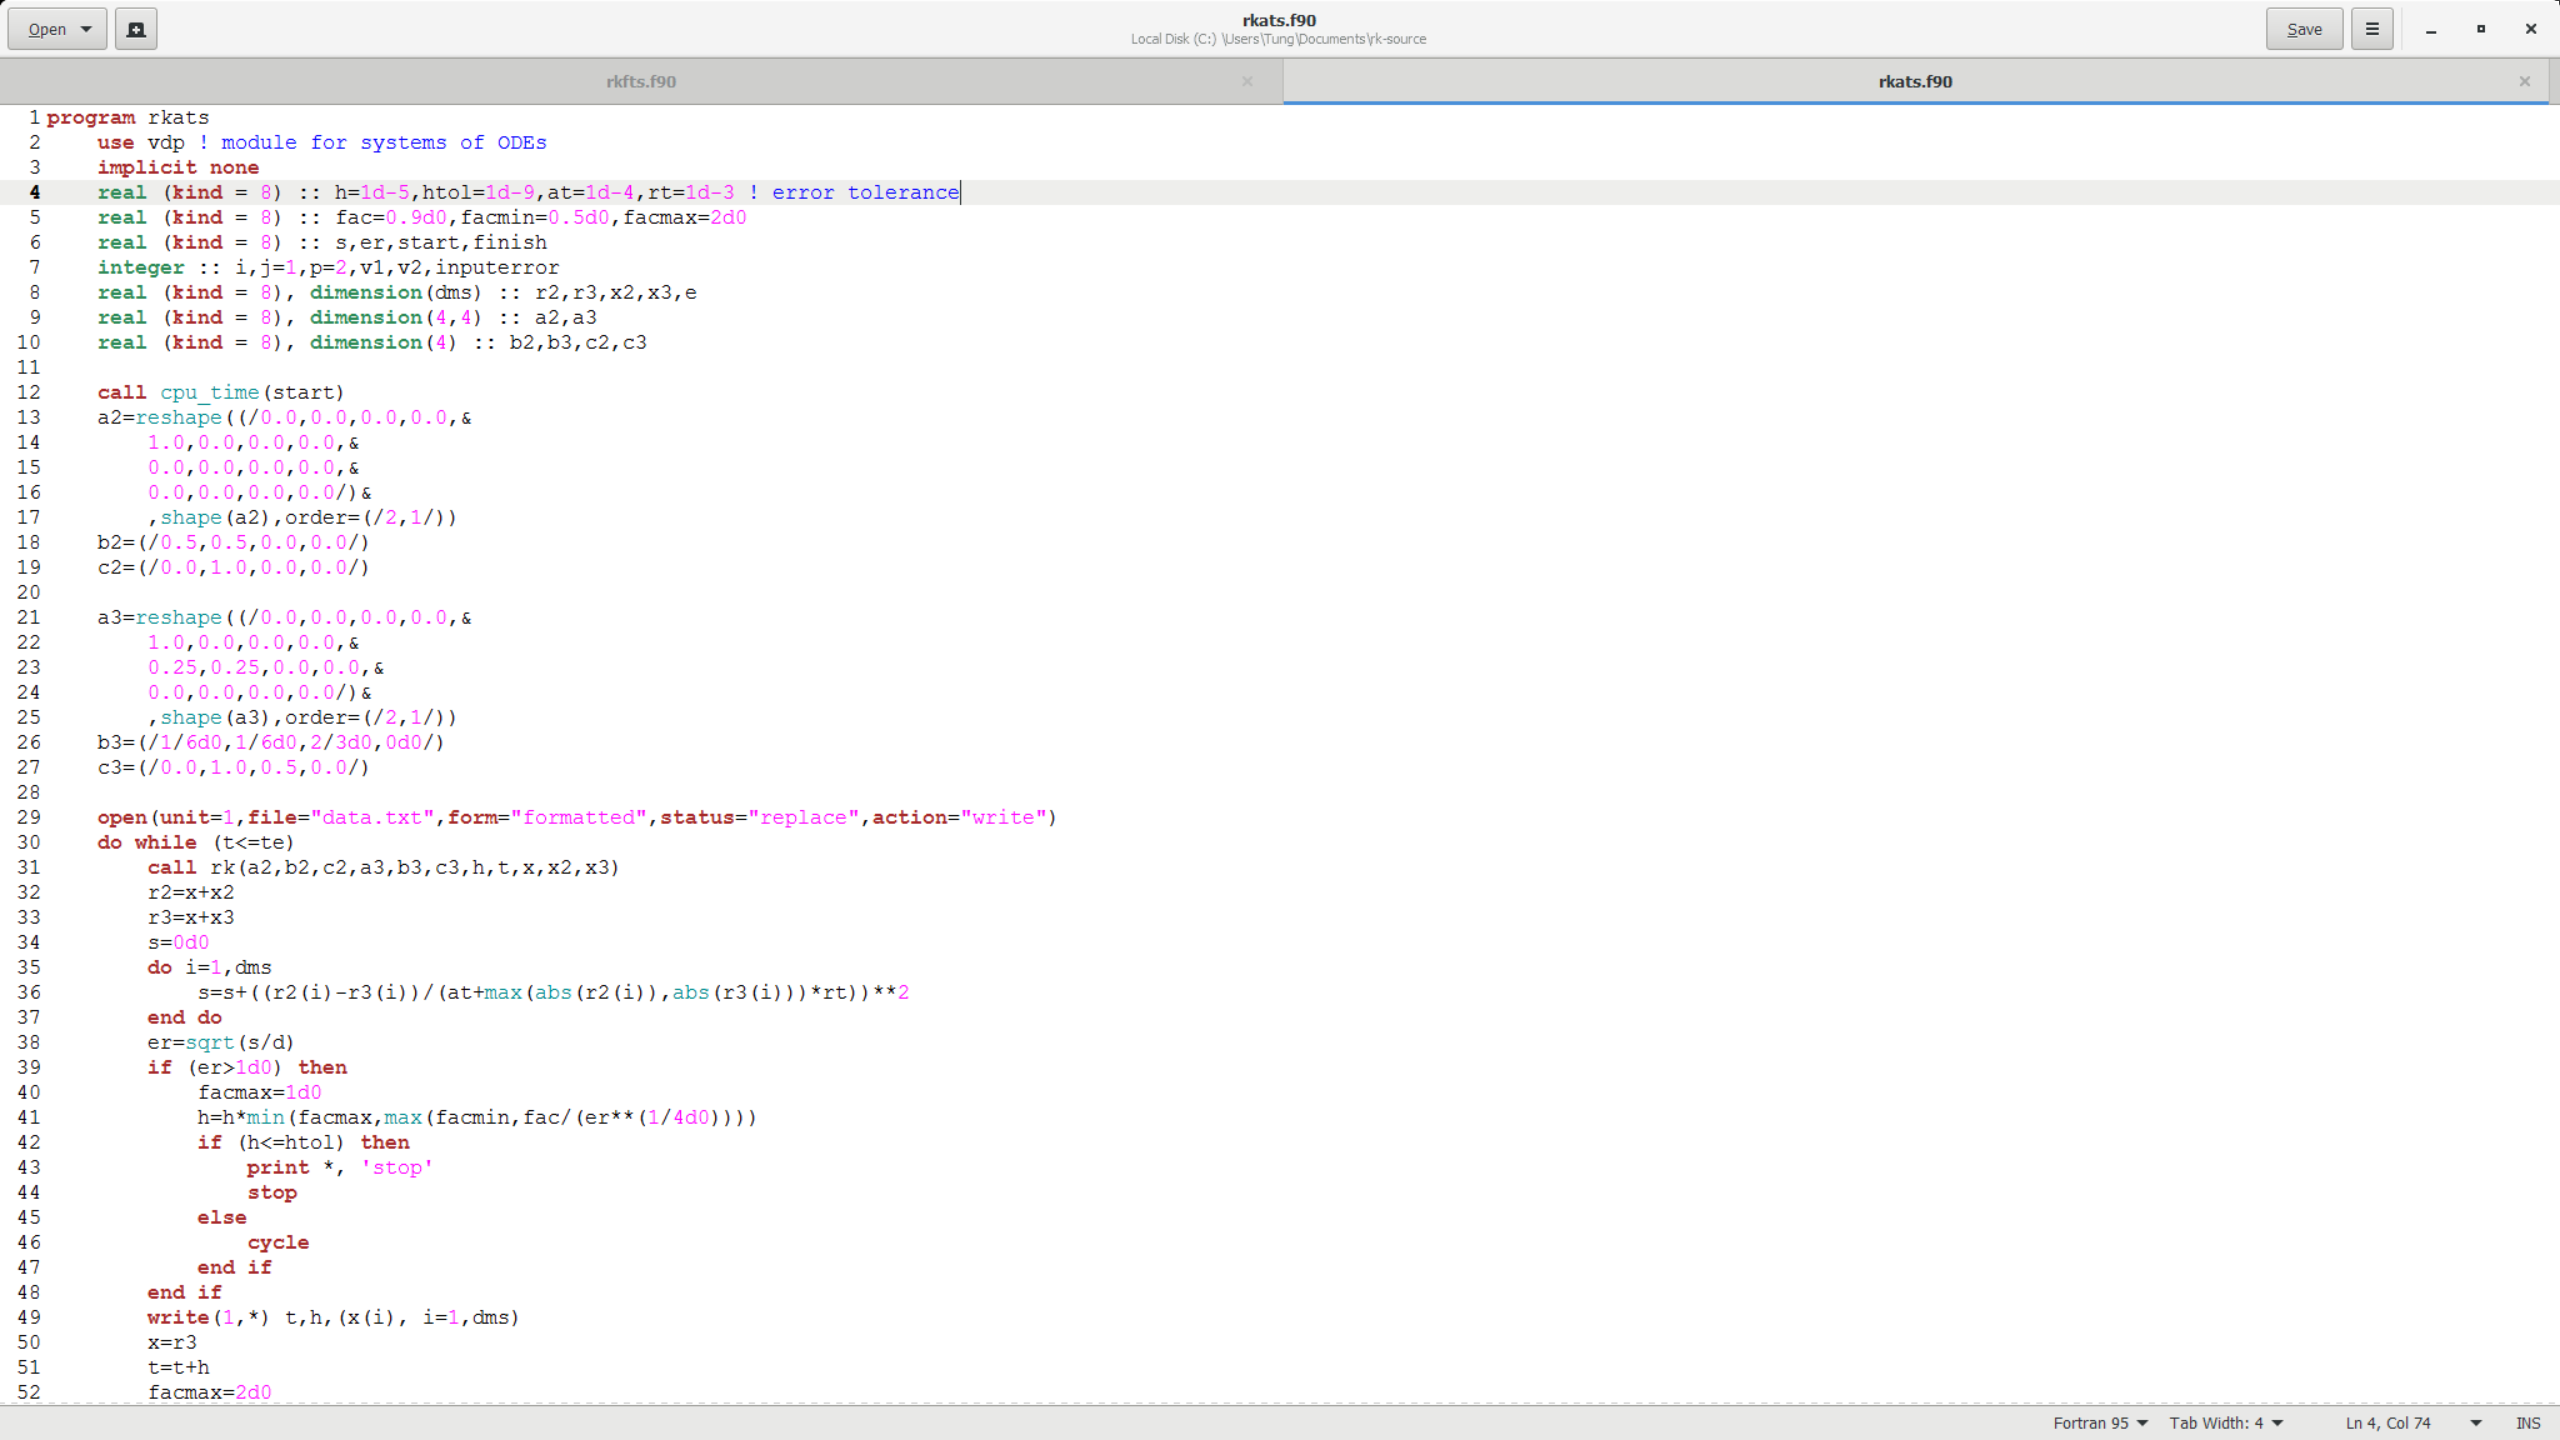
\includegraphics[width=15cm]{fig02}
		\caption{rkats.f90}
	\end{figure}
	\section{Using the code}
	$\bullet$ \textbf{Step 1:} Decide which equation you want to solve and whether you want to solve it using Runge-Kutta method with fixed time step or adaptive time step. Put the file containing the module specifies that equation and the file corresponding to the method of your choice together with \texttt{data\_plot.plt} and \texttt{data\_plot\_dependency.plt} in a same folder.\\\\
	\textbf{For example:} You want to solve the Van der Pol equation specified in \texttt{vfp.f90} using Runge-Kutta method with adaptive time step, you need to put \texttt{rkats.f90}, \texttt{vdp.f90}, \texttt{data\_plot.plt} and \texttt{data\_plot\_dependency.plt} in the same folder. From now on, we will use this example for sake of convenience.
	\begin{figure}[H]
		\centering	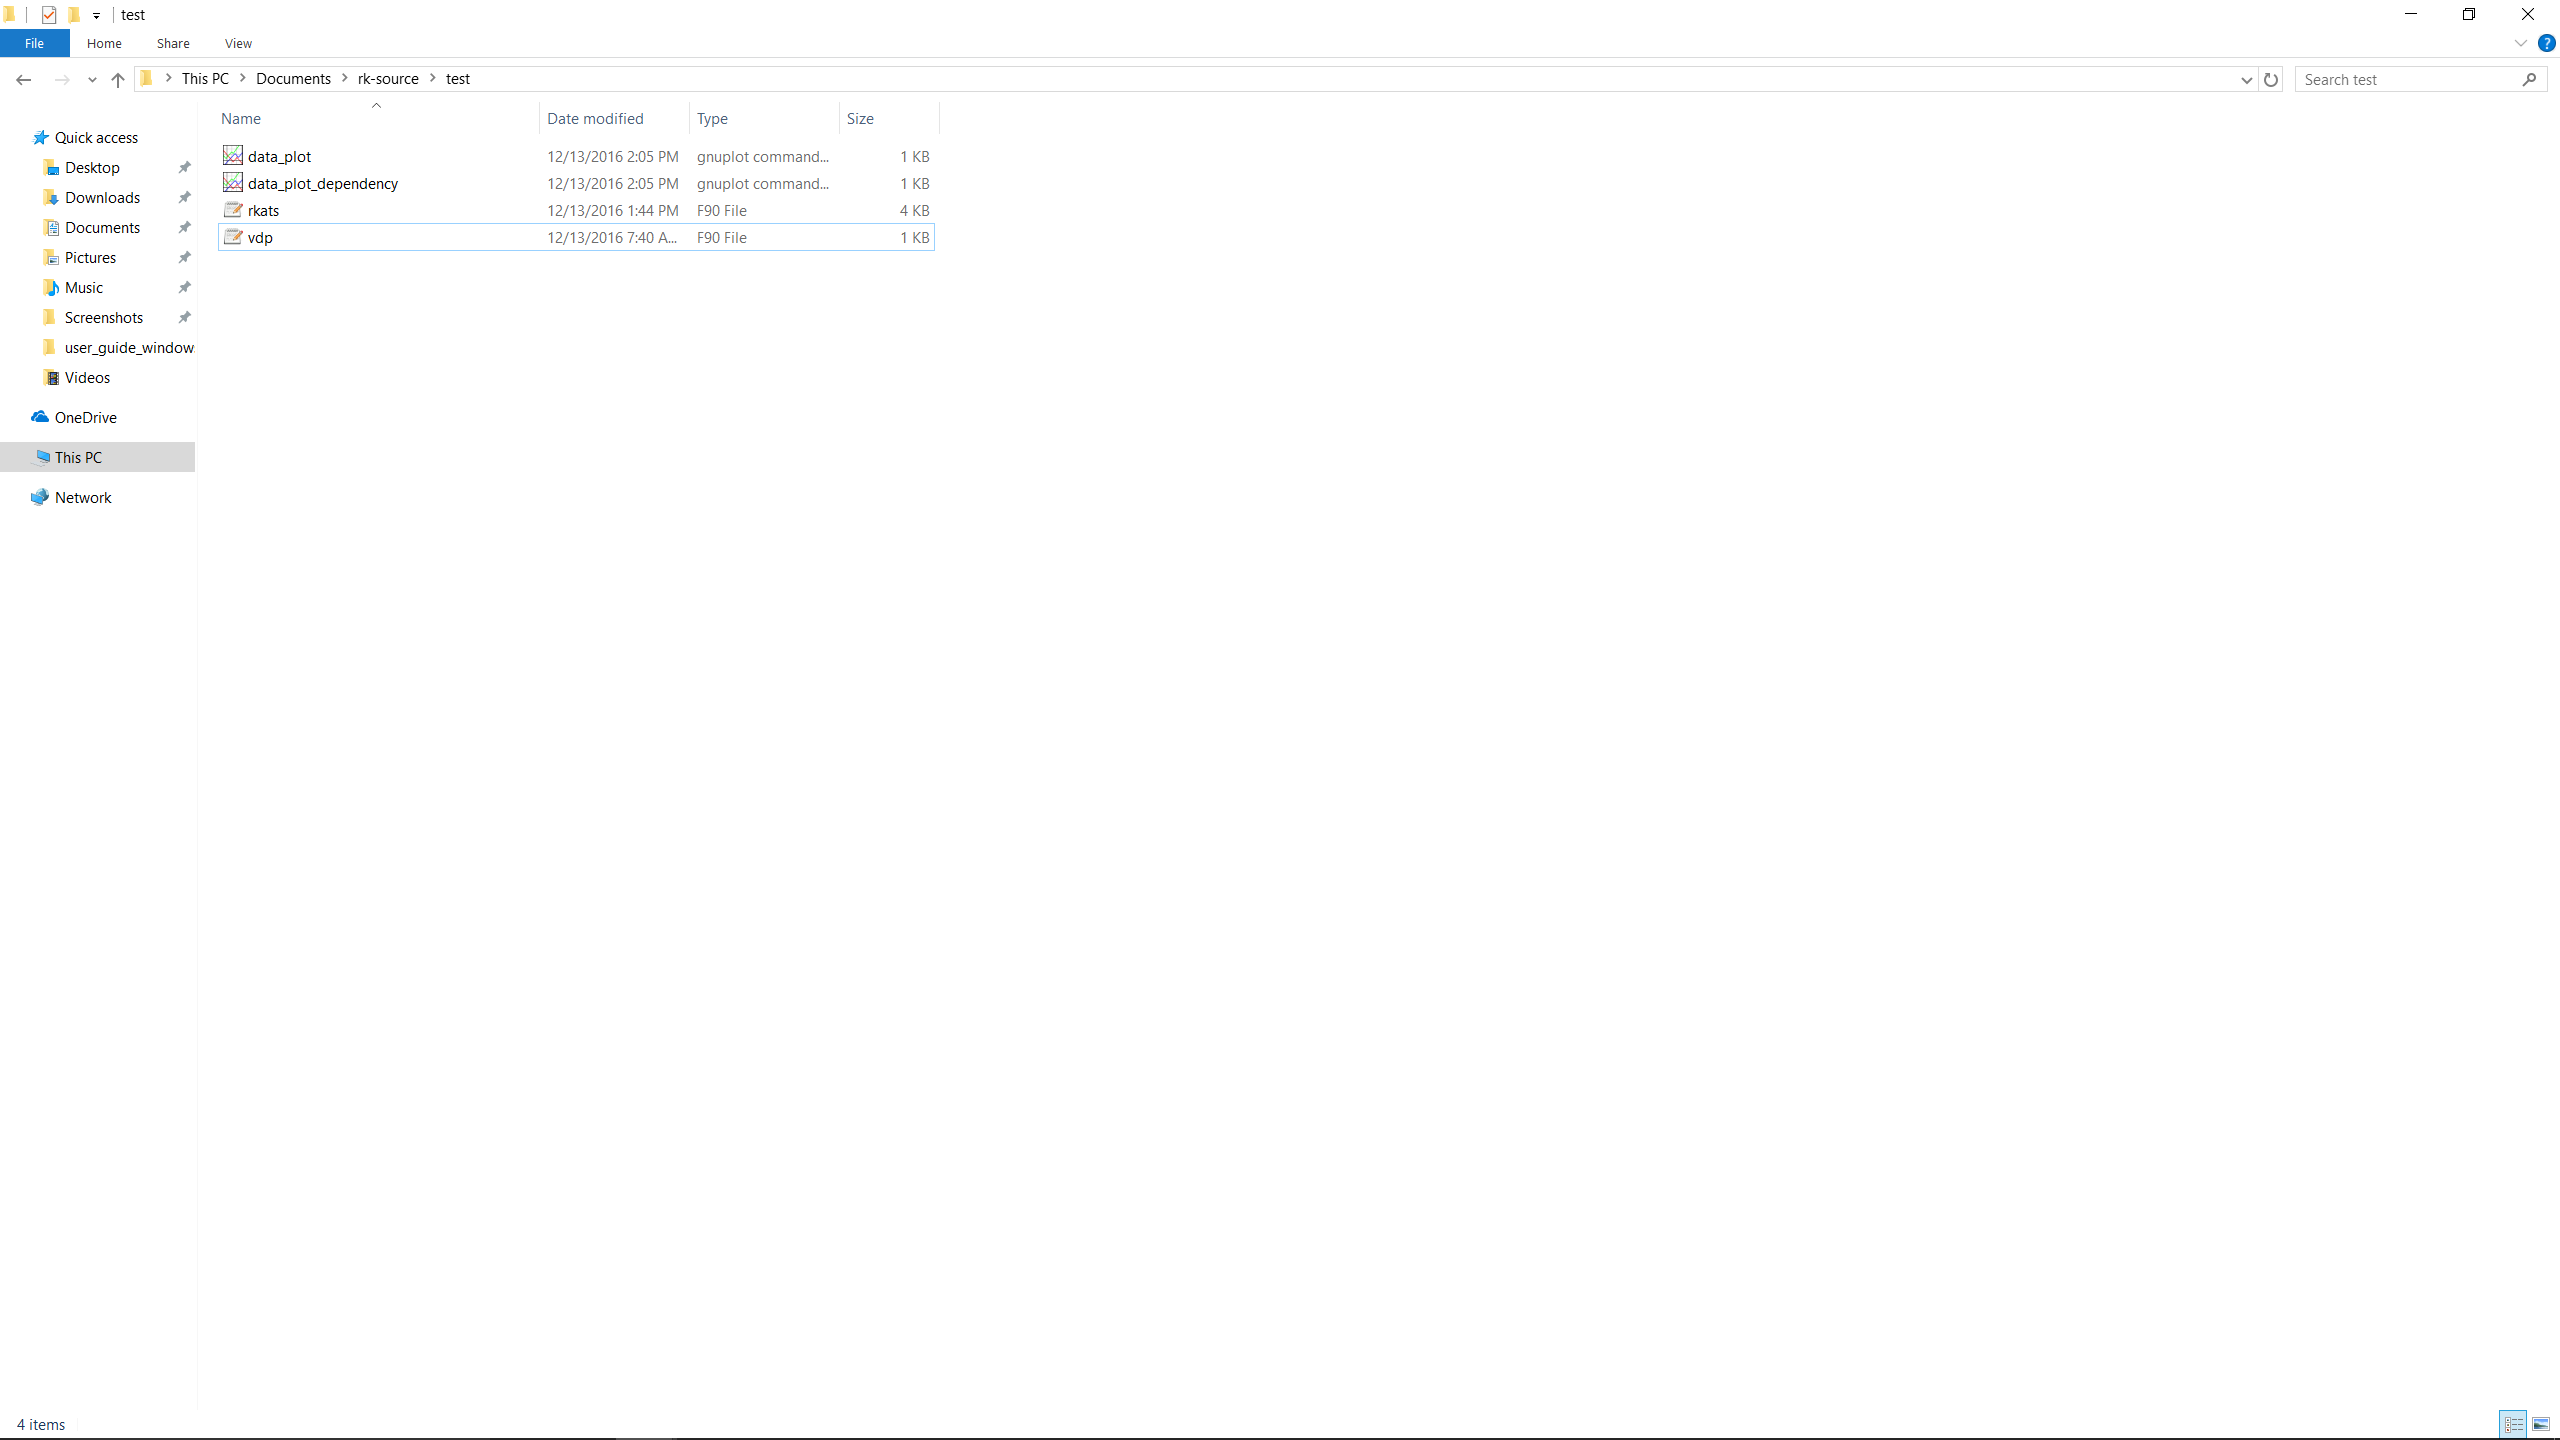
\includegraphics[width=15cm]{fig1}
		\caption{Put the needed files in the same folder}
	\end{figure}
	\noindent$\bullet$ \textbf{Step 2:} Open the folder in \textbf{Command Prompt}
	\begin{figure}[H]
		\centering	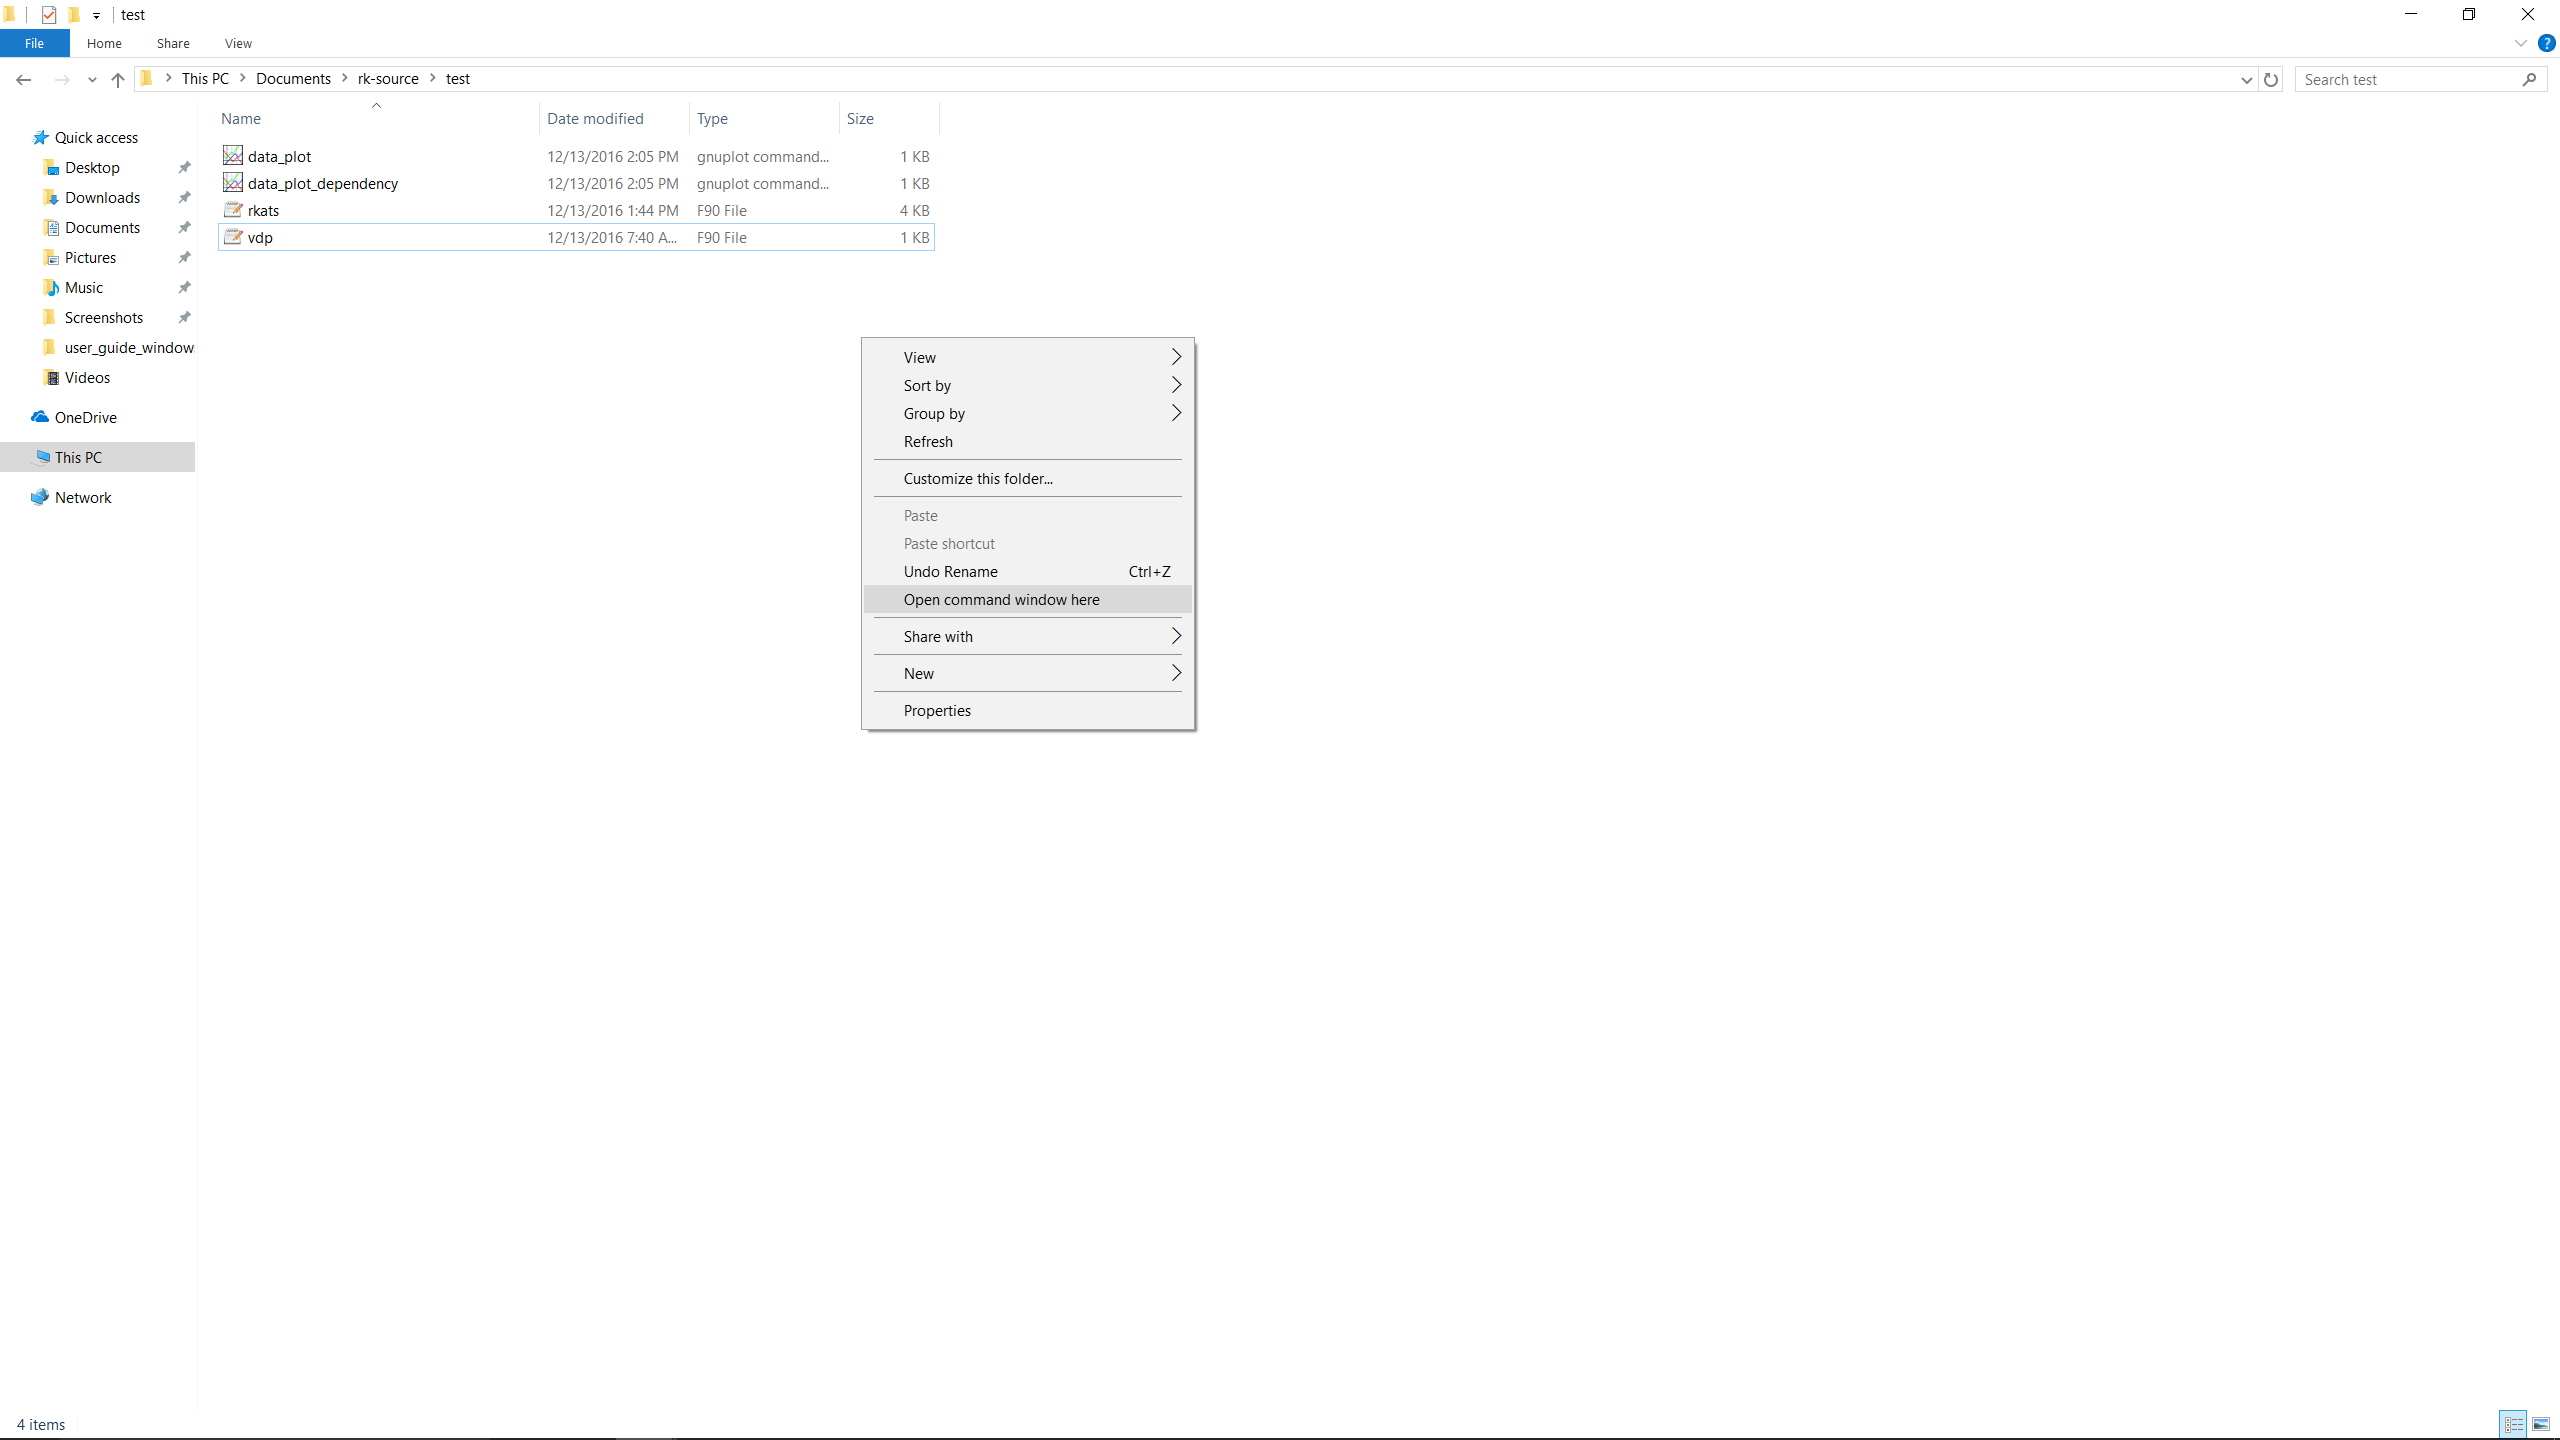
\includegraphics[width=15cm]{fig2}
		\caption{Press \textbf{Shift + Right click} at the empty space and select \texttt{Open command window here}}
	\end{figure}
	\begin{figure}[H]
		\centering	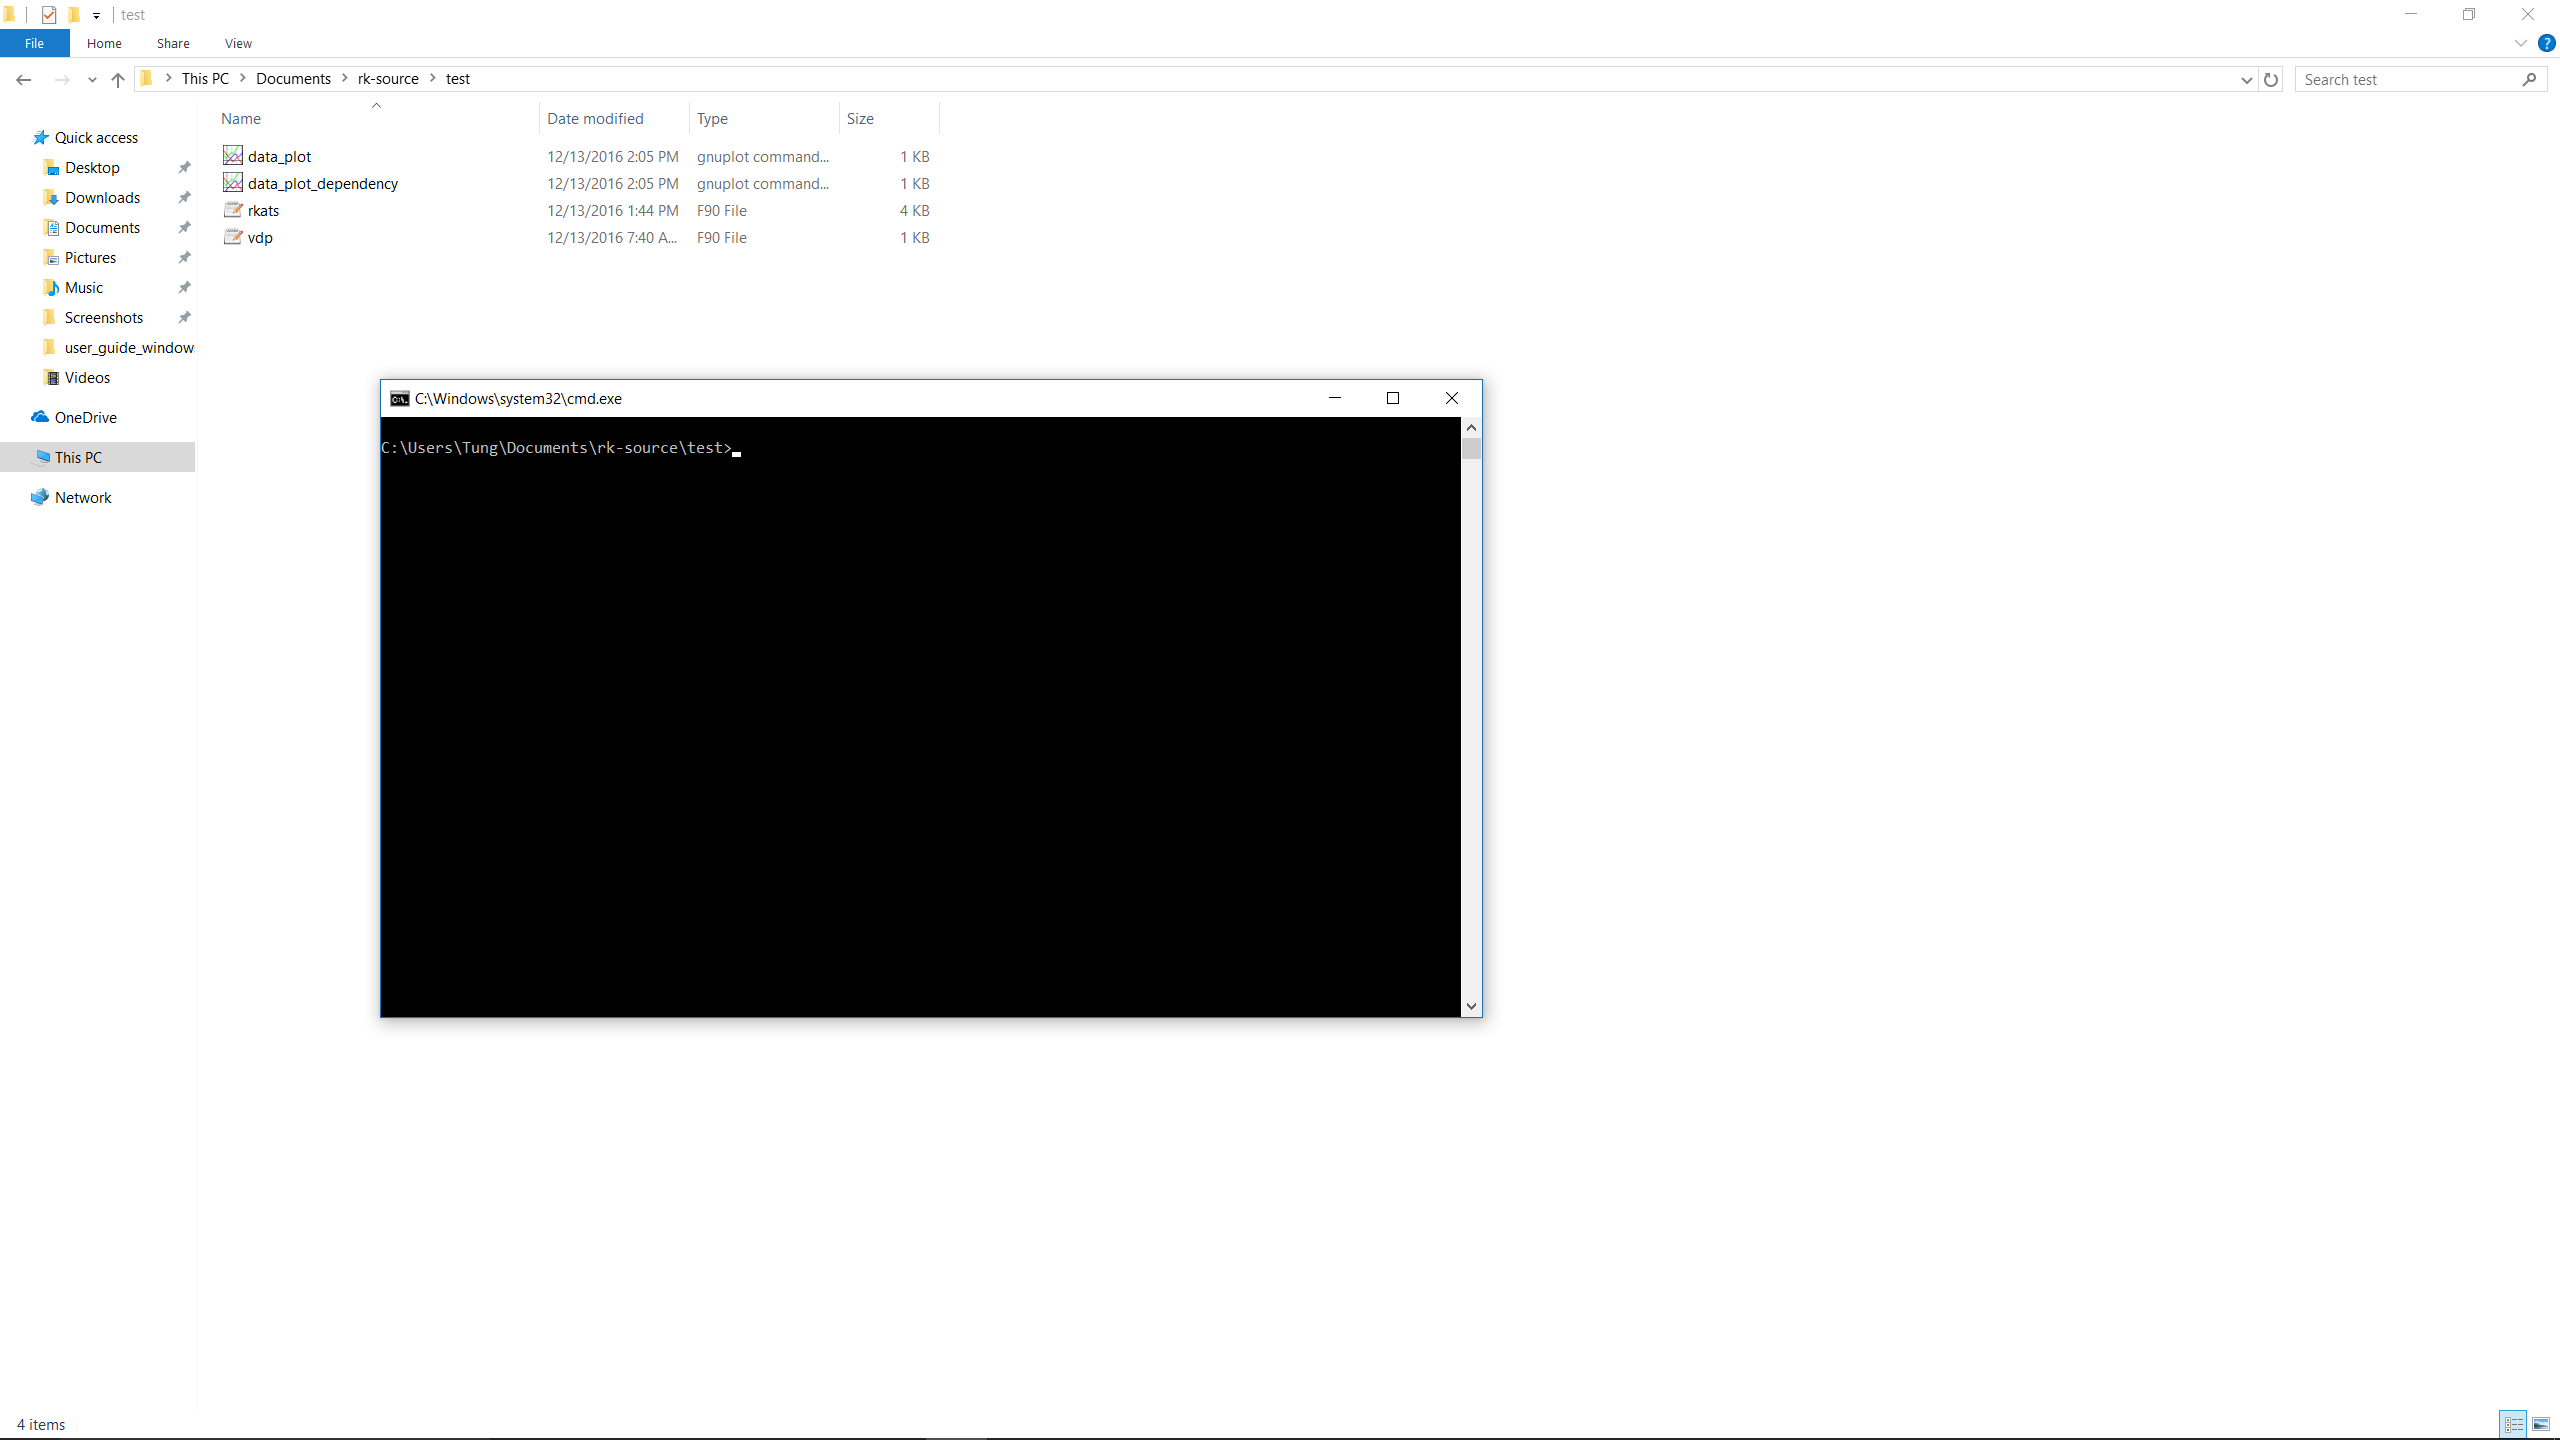
\includegraphics[width=15cm]{fig3}
		\caption{The folder is now opened in Command Prompt}
	\end{figure}
	\noindent$\bullet$ \textbf{Step 3:} Open \texttt{rkats.f90} in a text editor and make sure that it use the module for your equation of choice (\texttt{vdp.f90} for the Van der Pol equation in this example) by modifying the second line: from \texttt{use [something]} to \texttt{use vdp}
	\begin{figure}[H]
		\centering	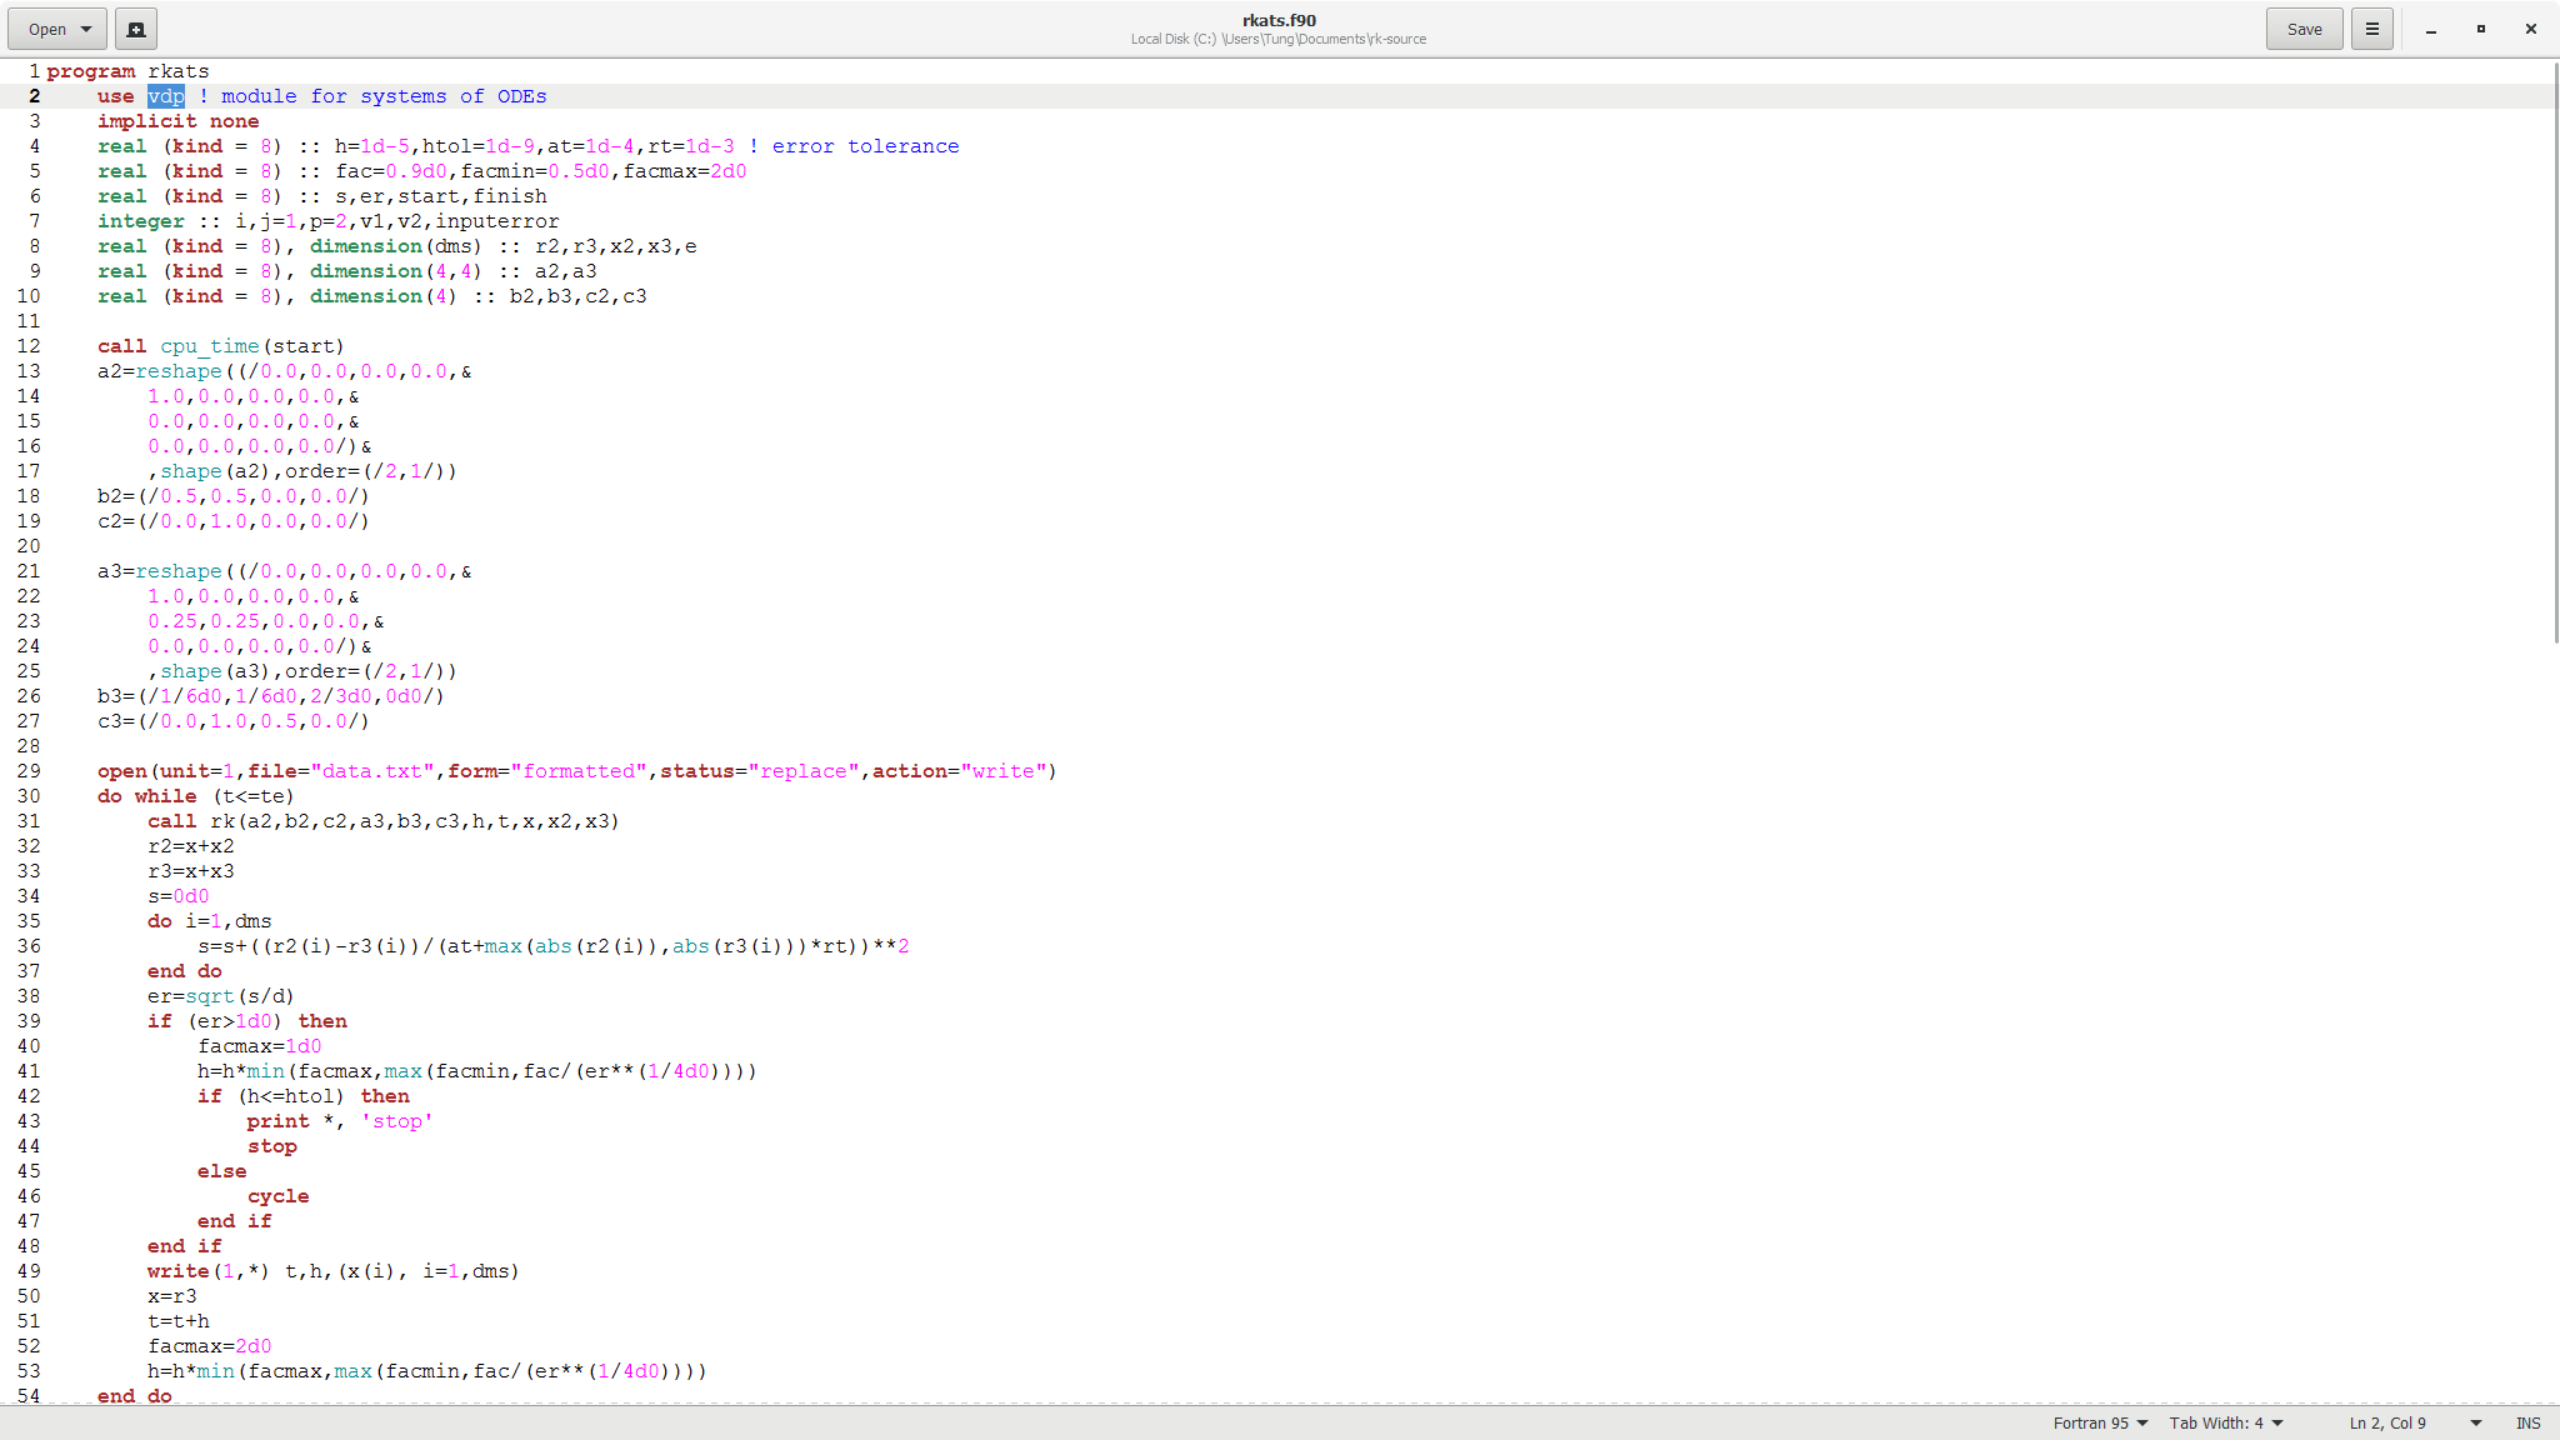
\includegraphics[width=15cm]{fig4}
		\caption{The result look like this}
	\end{figure}
	\noindent$\bullet$ \textbf{Step 4:} Type \texttt{gfortran vdp.f90 rkats.f90 -o main.out} to make the output file named \texttt{main.out}, of course you can choose other names as well.
	\begin{figure}[H]
		\centering	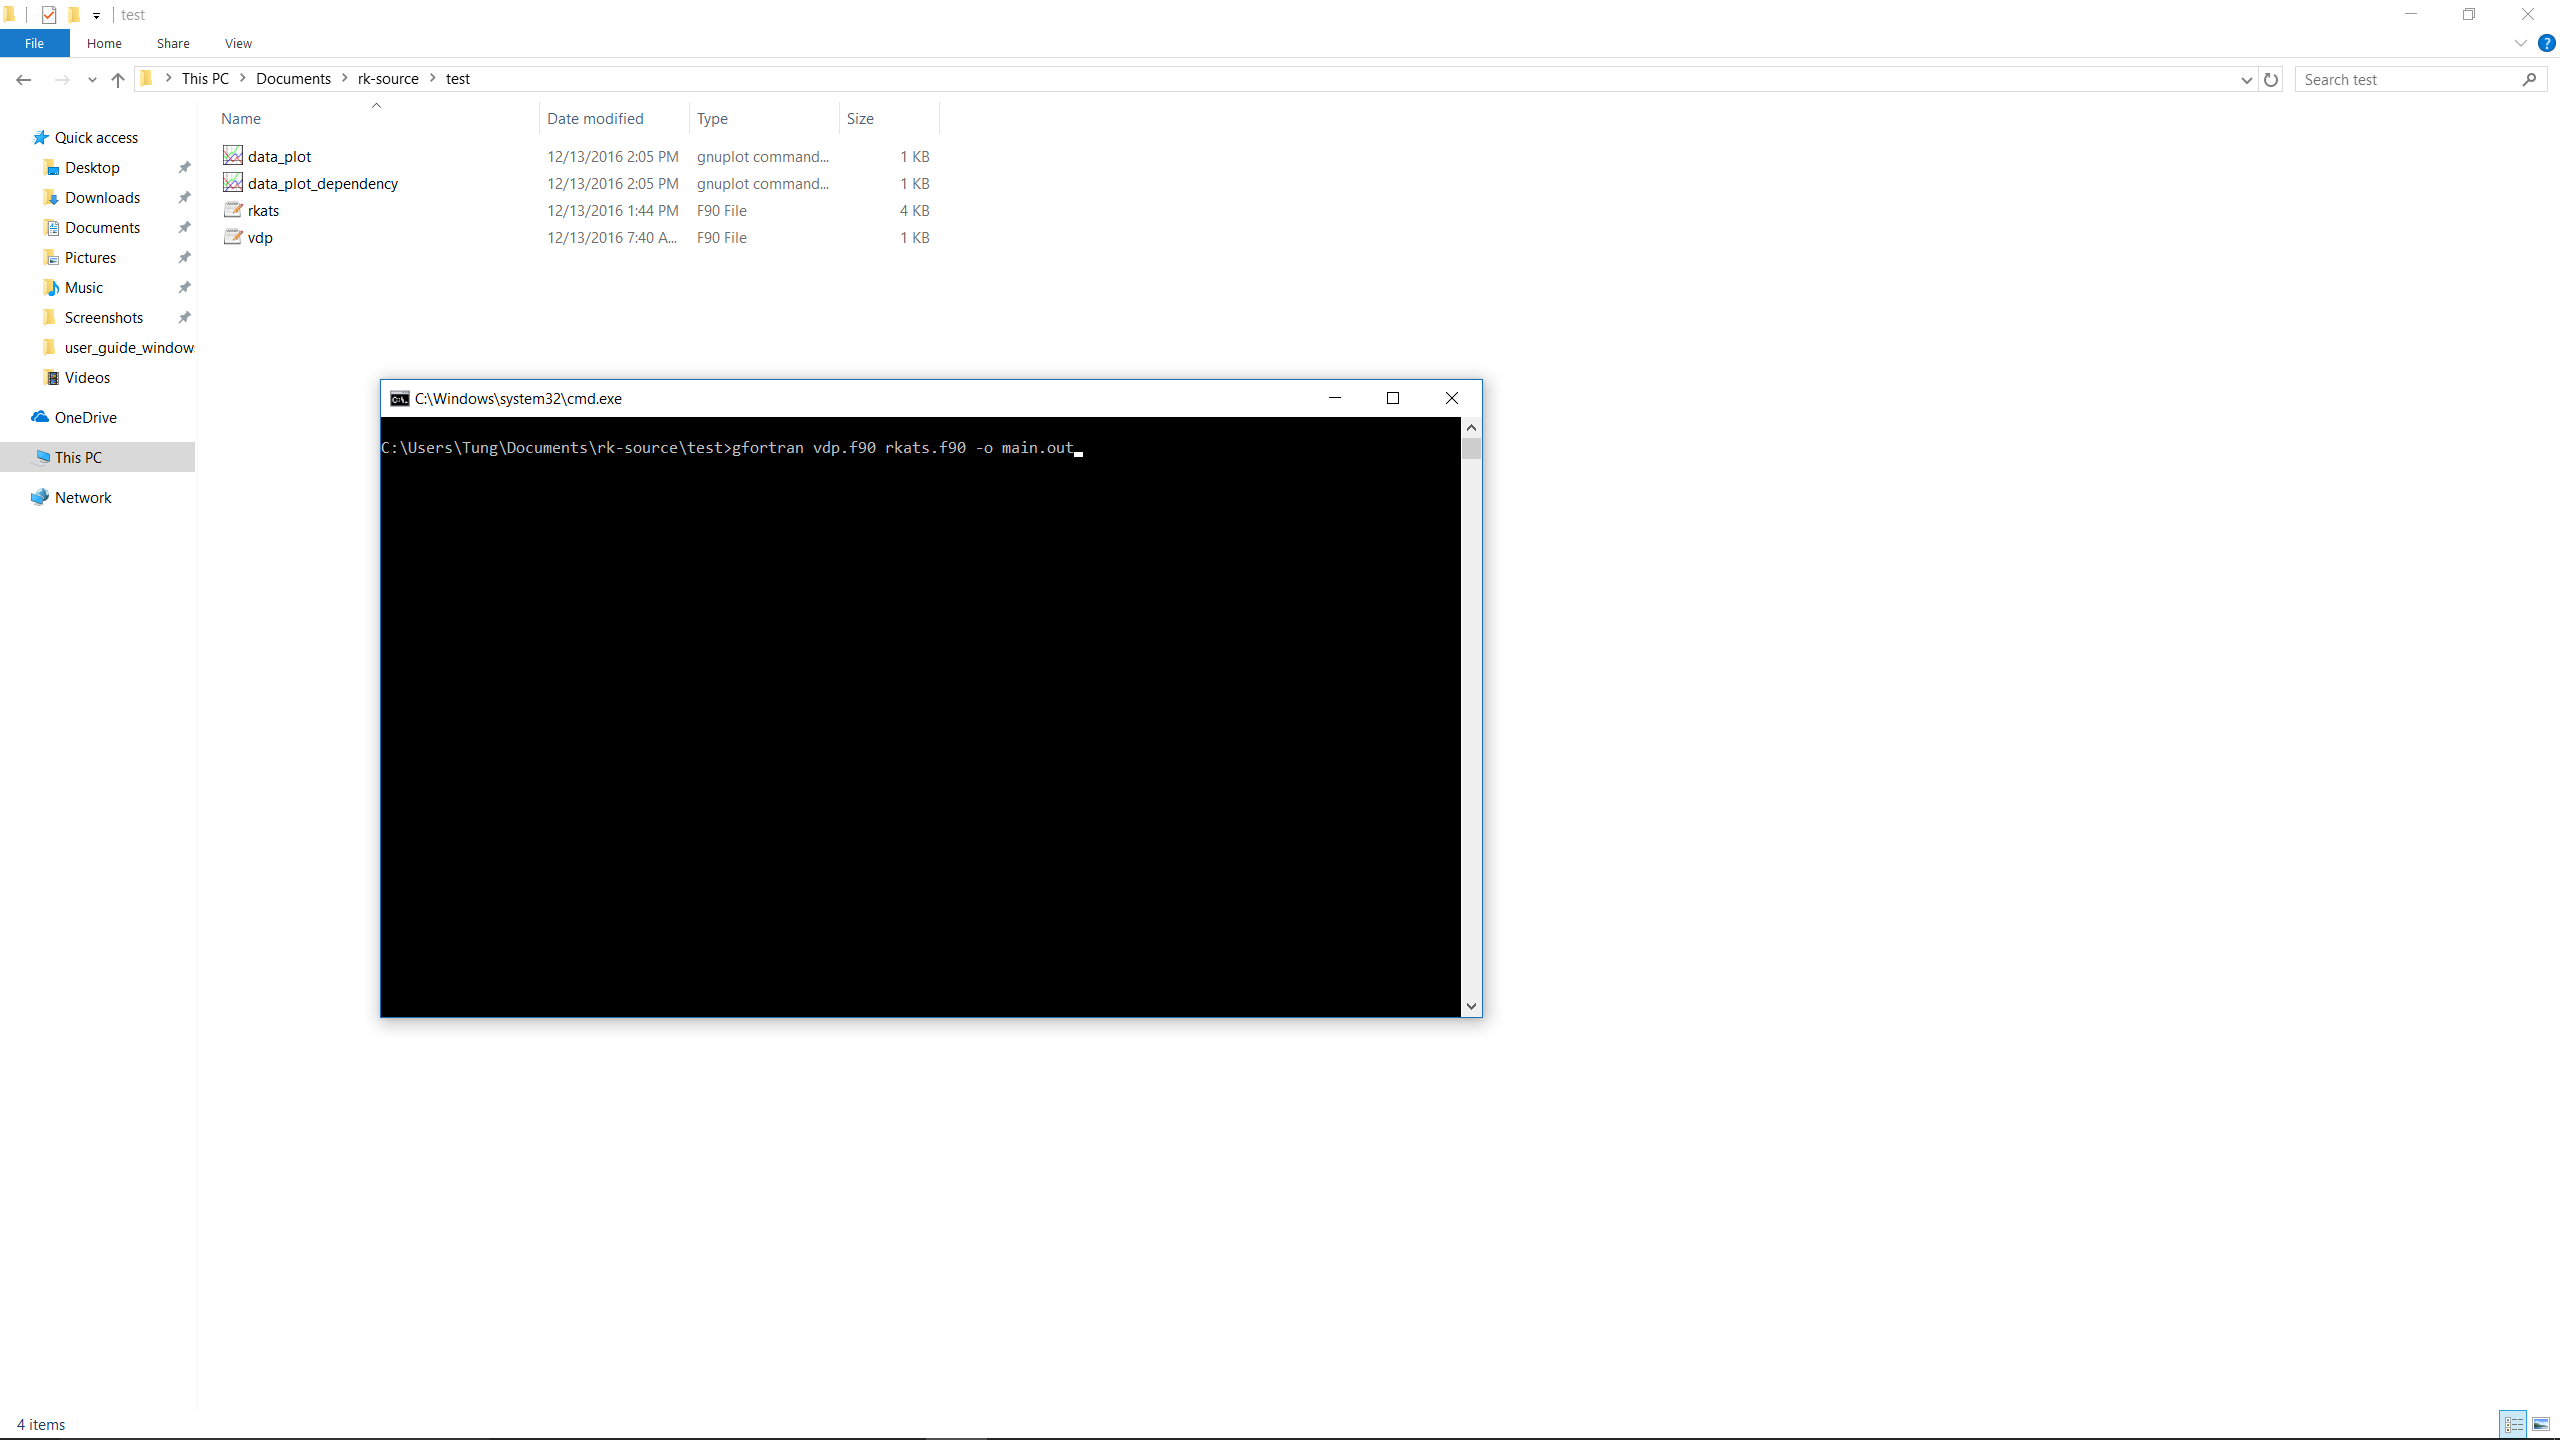
\includegraphics[width=15cm]{fig5}
		\caption{Typing the command in the Command Prompt}
	\end{figure}
	\begin{figure}[H]
		\centering	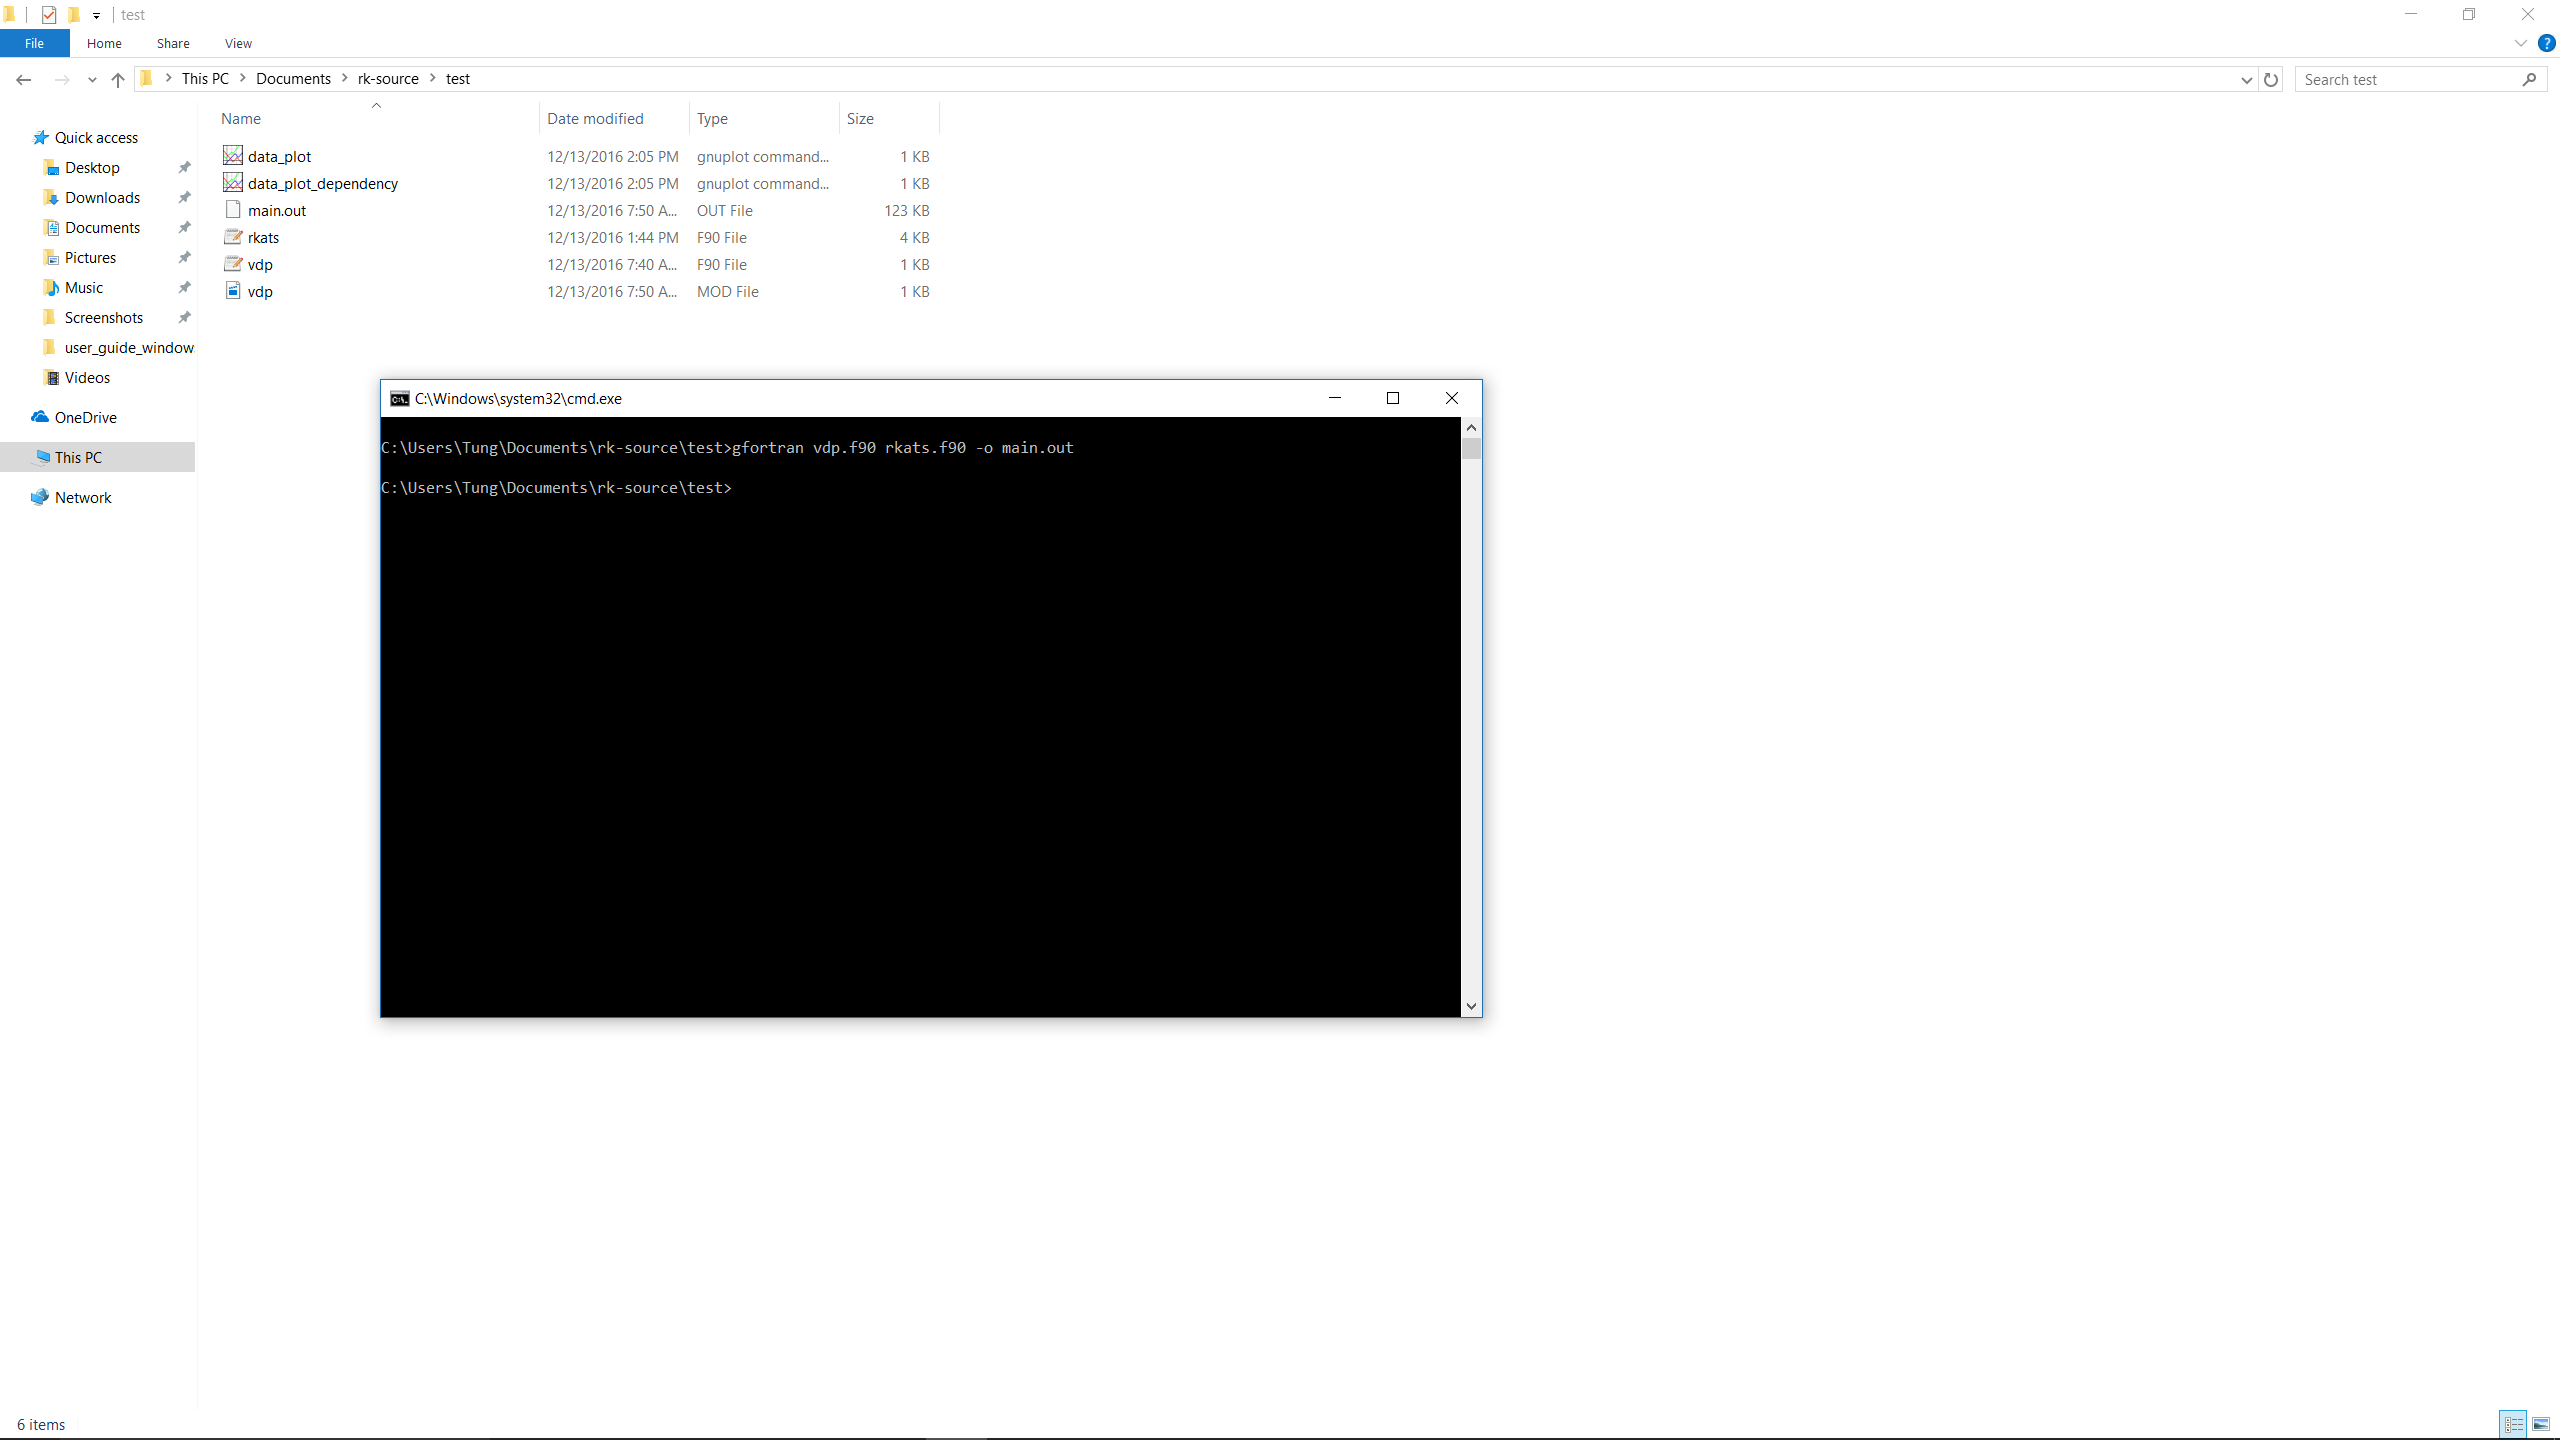
\includegraphics[width=15cm]{fig6}
		\caption{Completing the command will result in some new files}
	\end{figure}
	\noindent$\bullet$ \textbf{Step 5:} Type \texttt{.\textbackslash main.out} to run the file \texttt{main.out}
	\begin{figure}[H]
		\centering	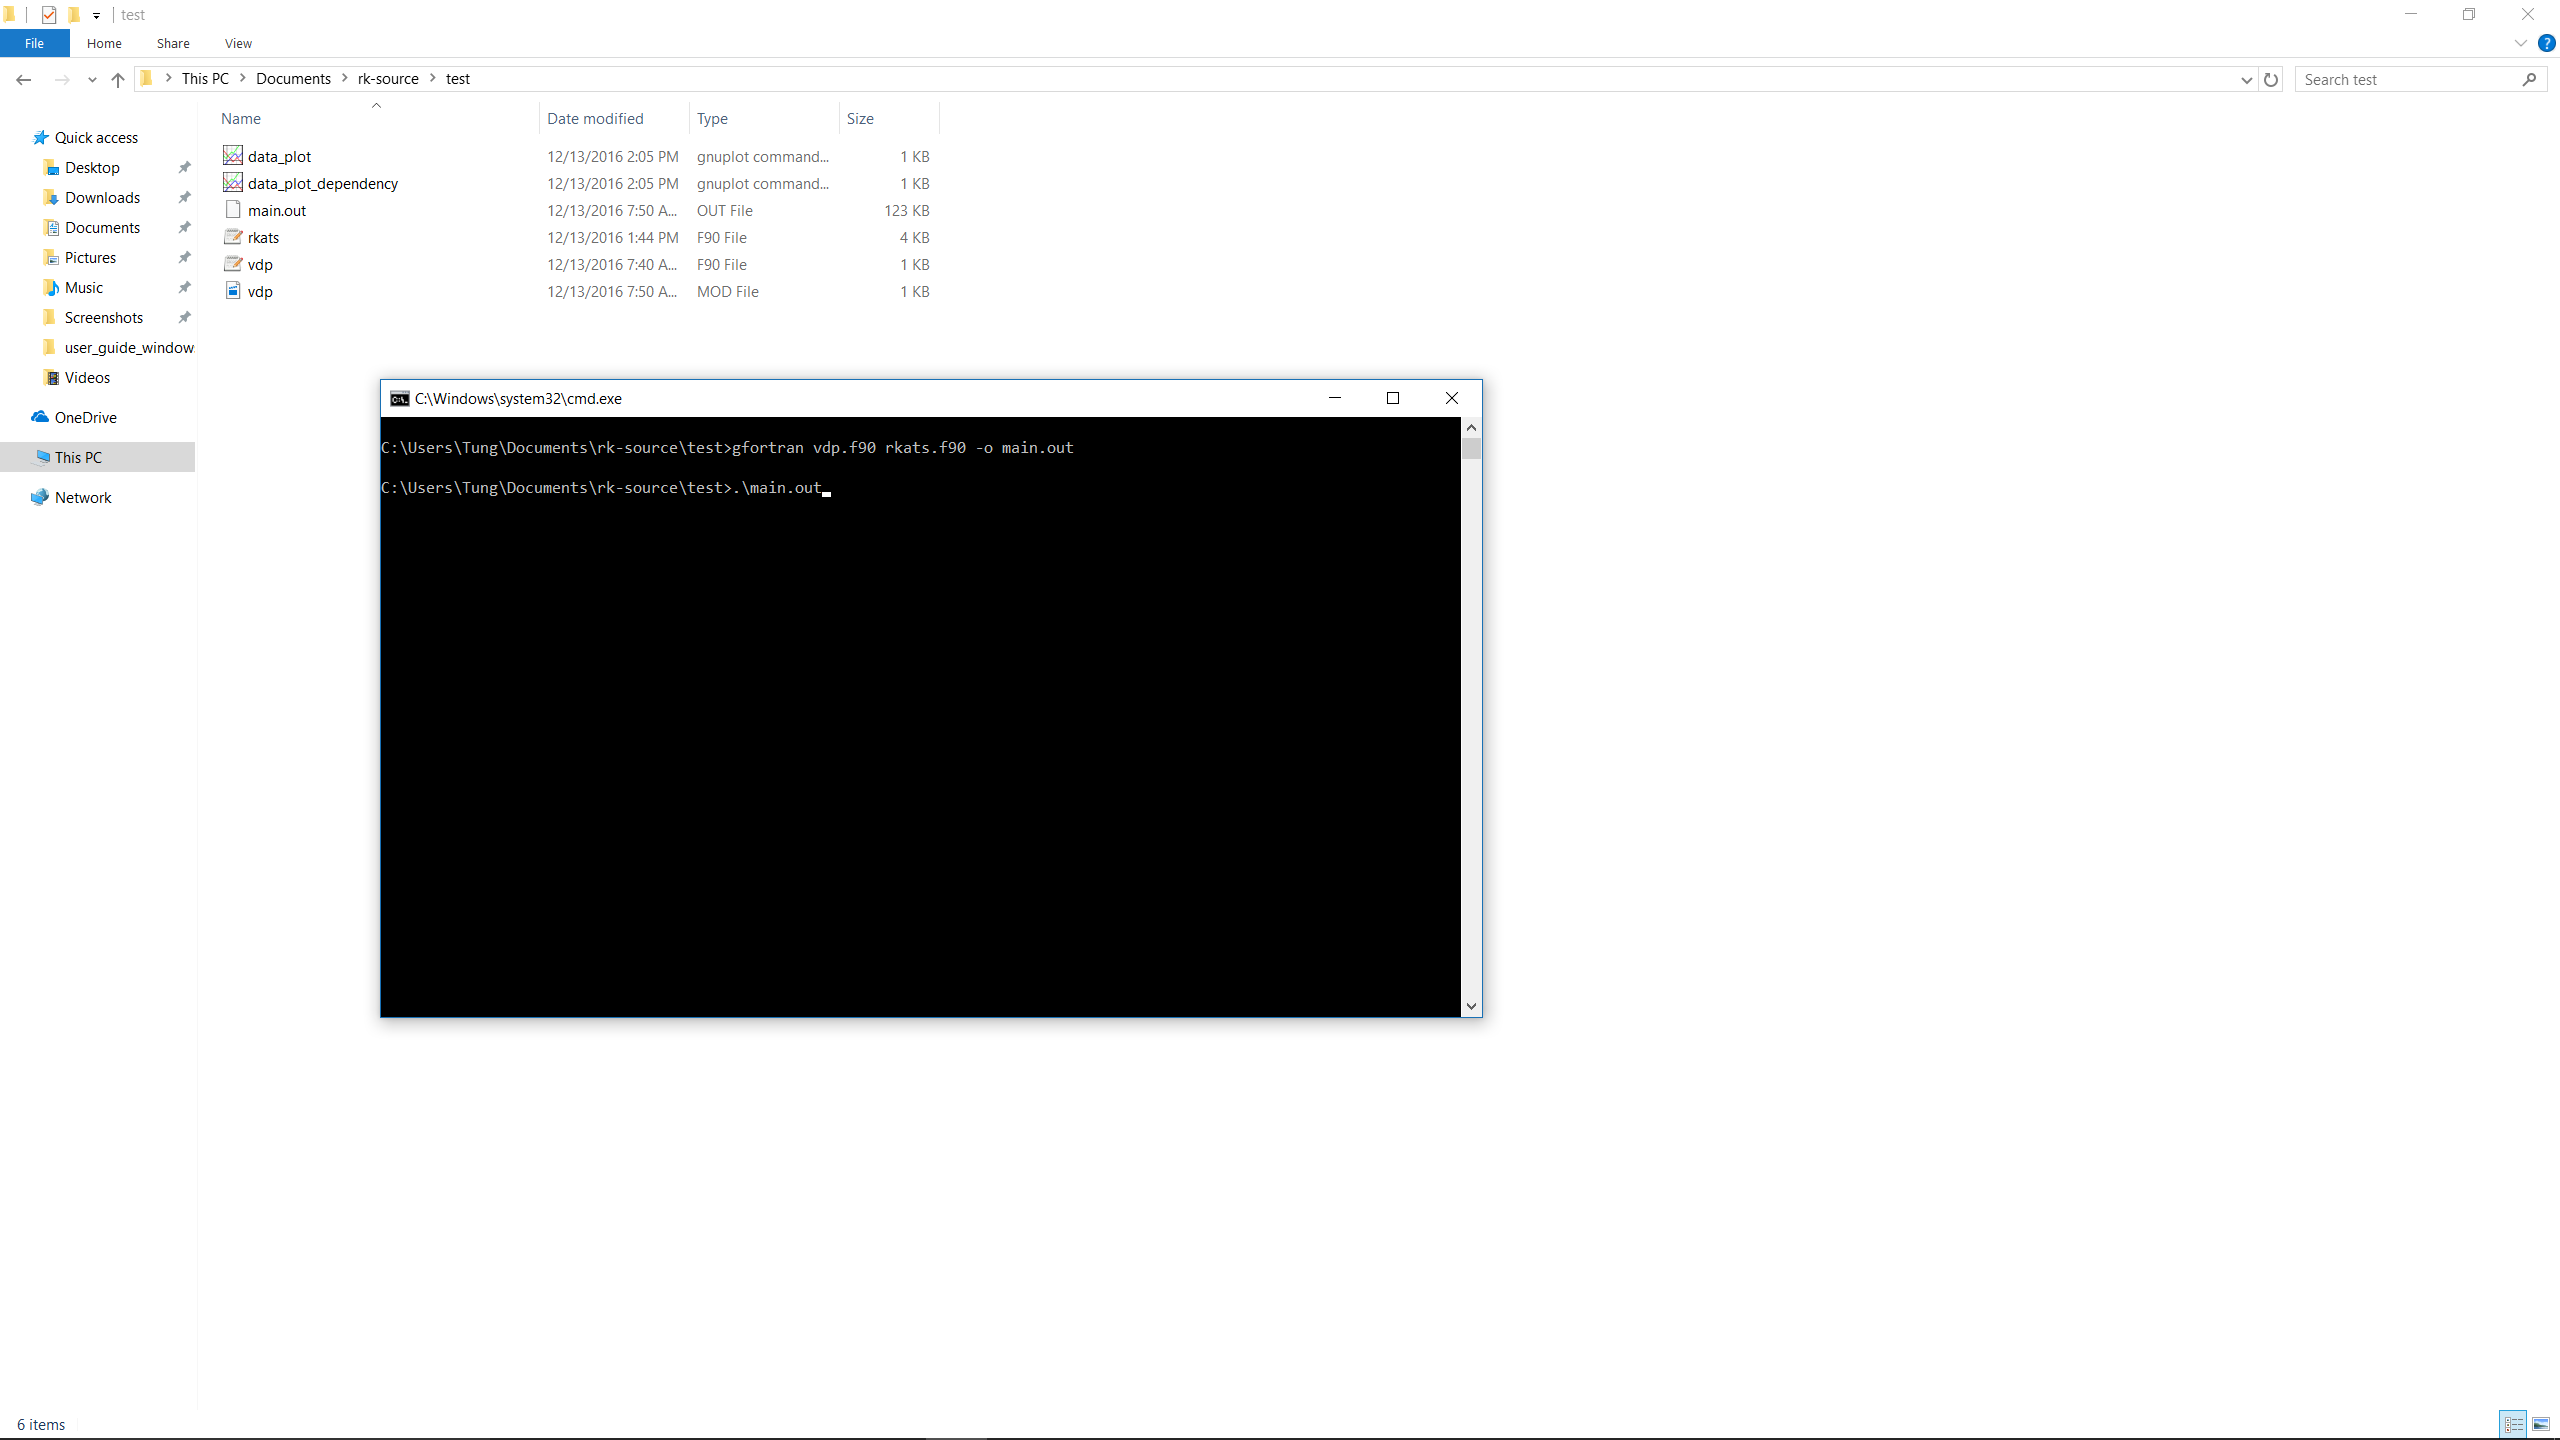
\includegraphics[width=15cm]{fig7}
		\caption{Typing the command in the Command Prompt}
	\end{figure}
	\noindent The command will run the program to solve the equation. The numerical result will be save into the file \texttt{data.txt} and the plots of the size of the step $h$ at time $t$ (only appear if you use adaptive time step method), the \textbf{solutions of the unknown variables of the equation} will appear, those plots would be saved in the same folder with the other file in the form of \texttt{*.pdf} and \texttt{*.tex} files. Additionally, several other files created by \texttt{gnuplot} are needed to compile the newly created \texttt{*.tex} files. 
	\begin{figure}[H]
		\centering	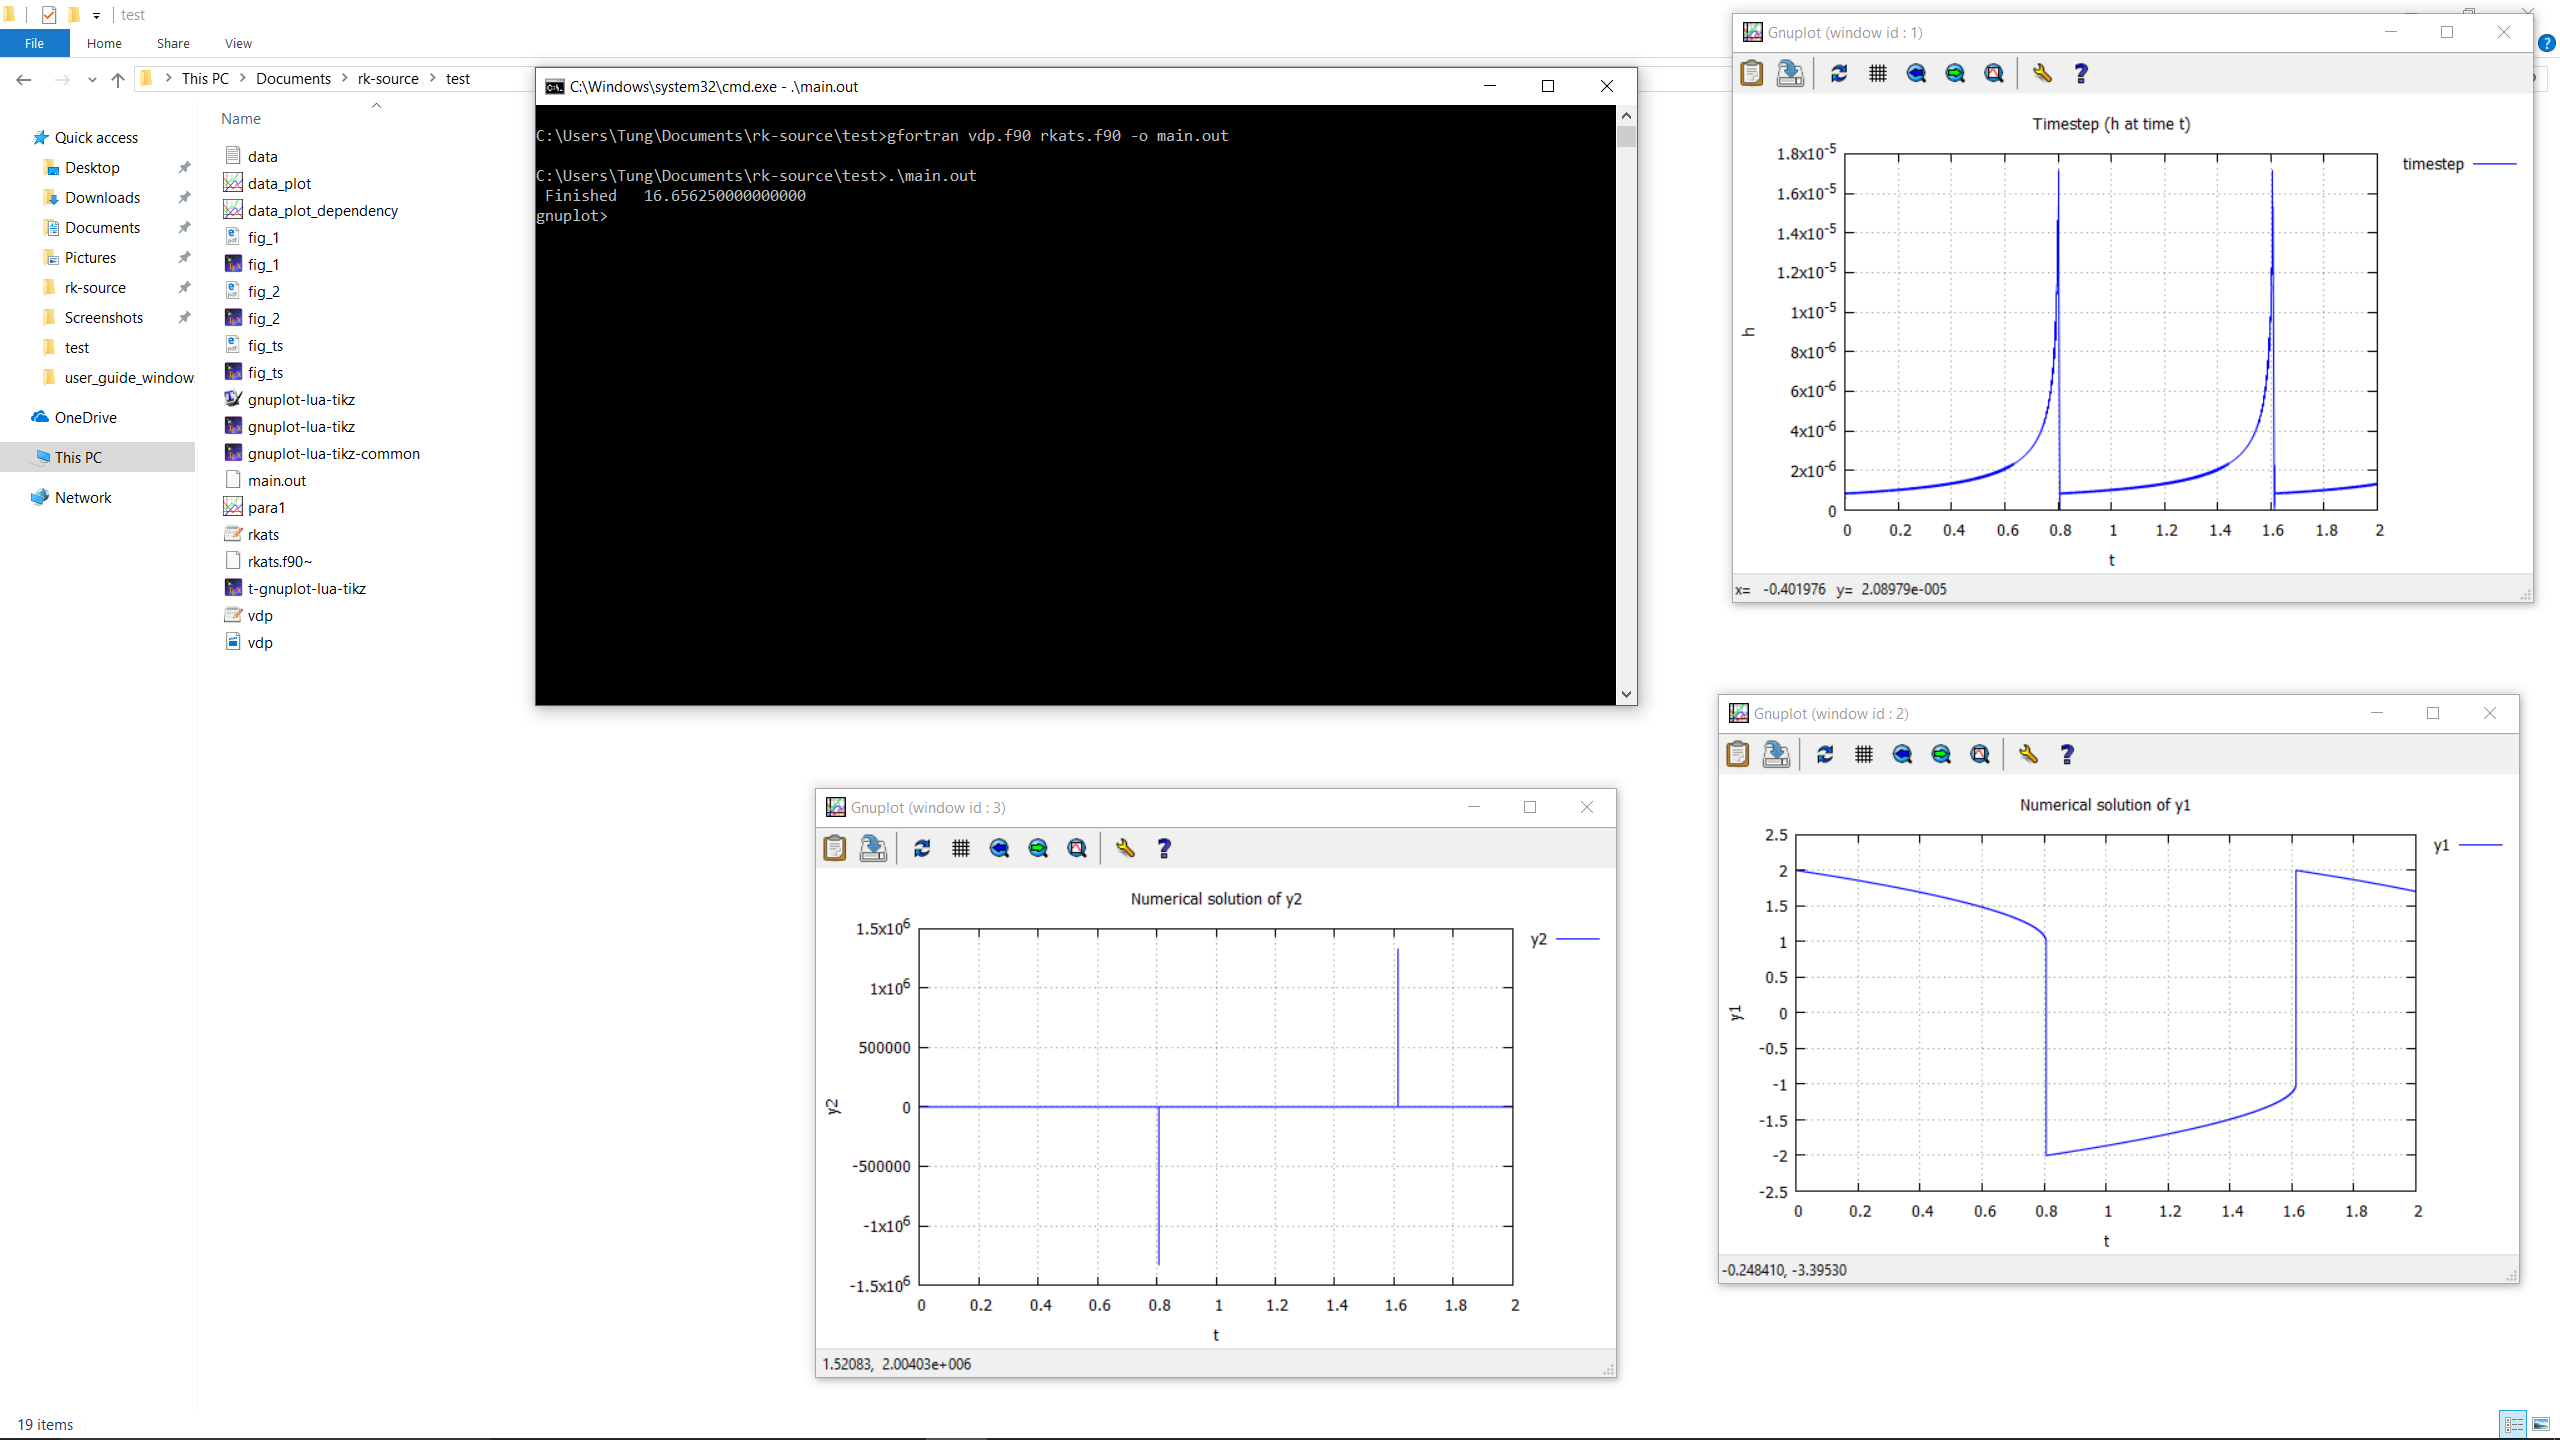
\includegraphics[width=15cm]{fig8}
		\caption{The result look like this}
	\end{figure}
	\noindent To continue, type \texttt{quit} in the Command Prompt to quit the current \texttt{gnuplot} windows
	\begin{figure}[H]
		\centering	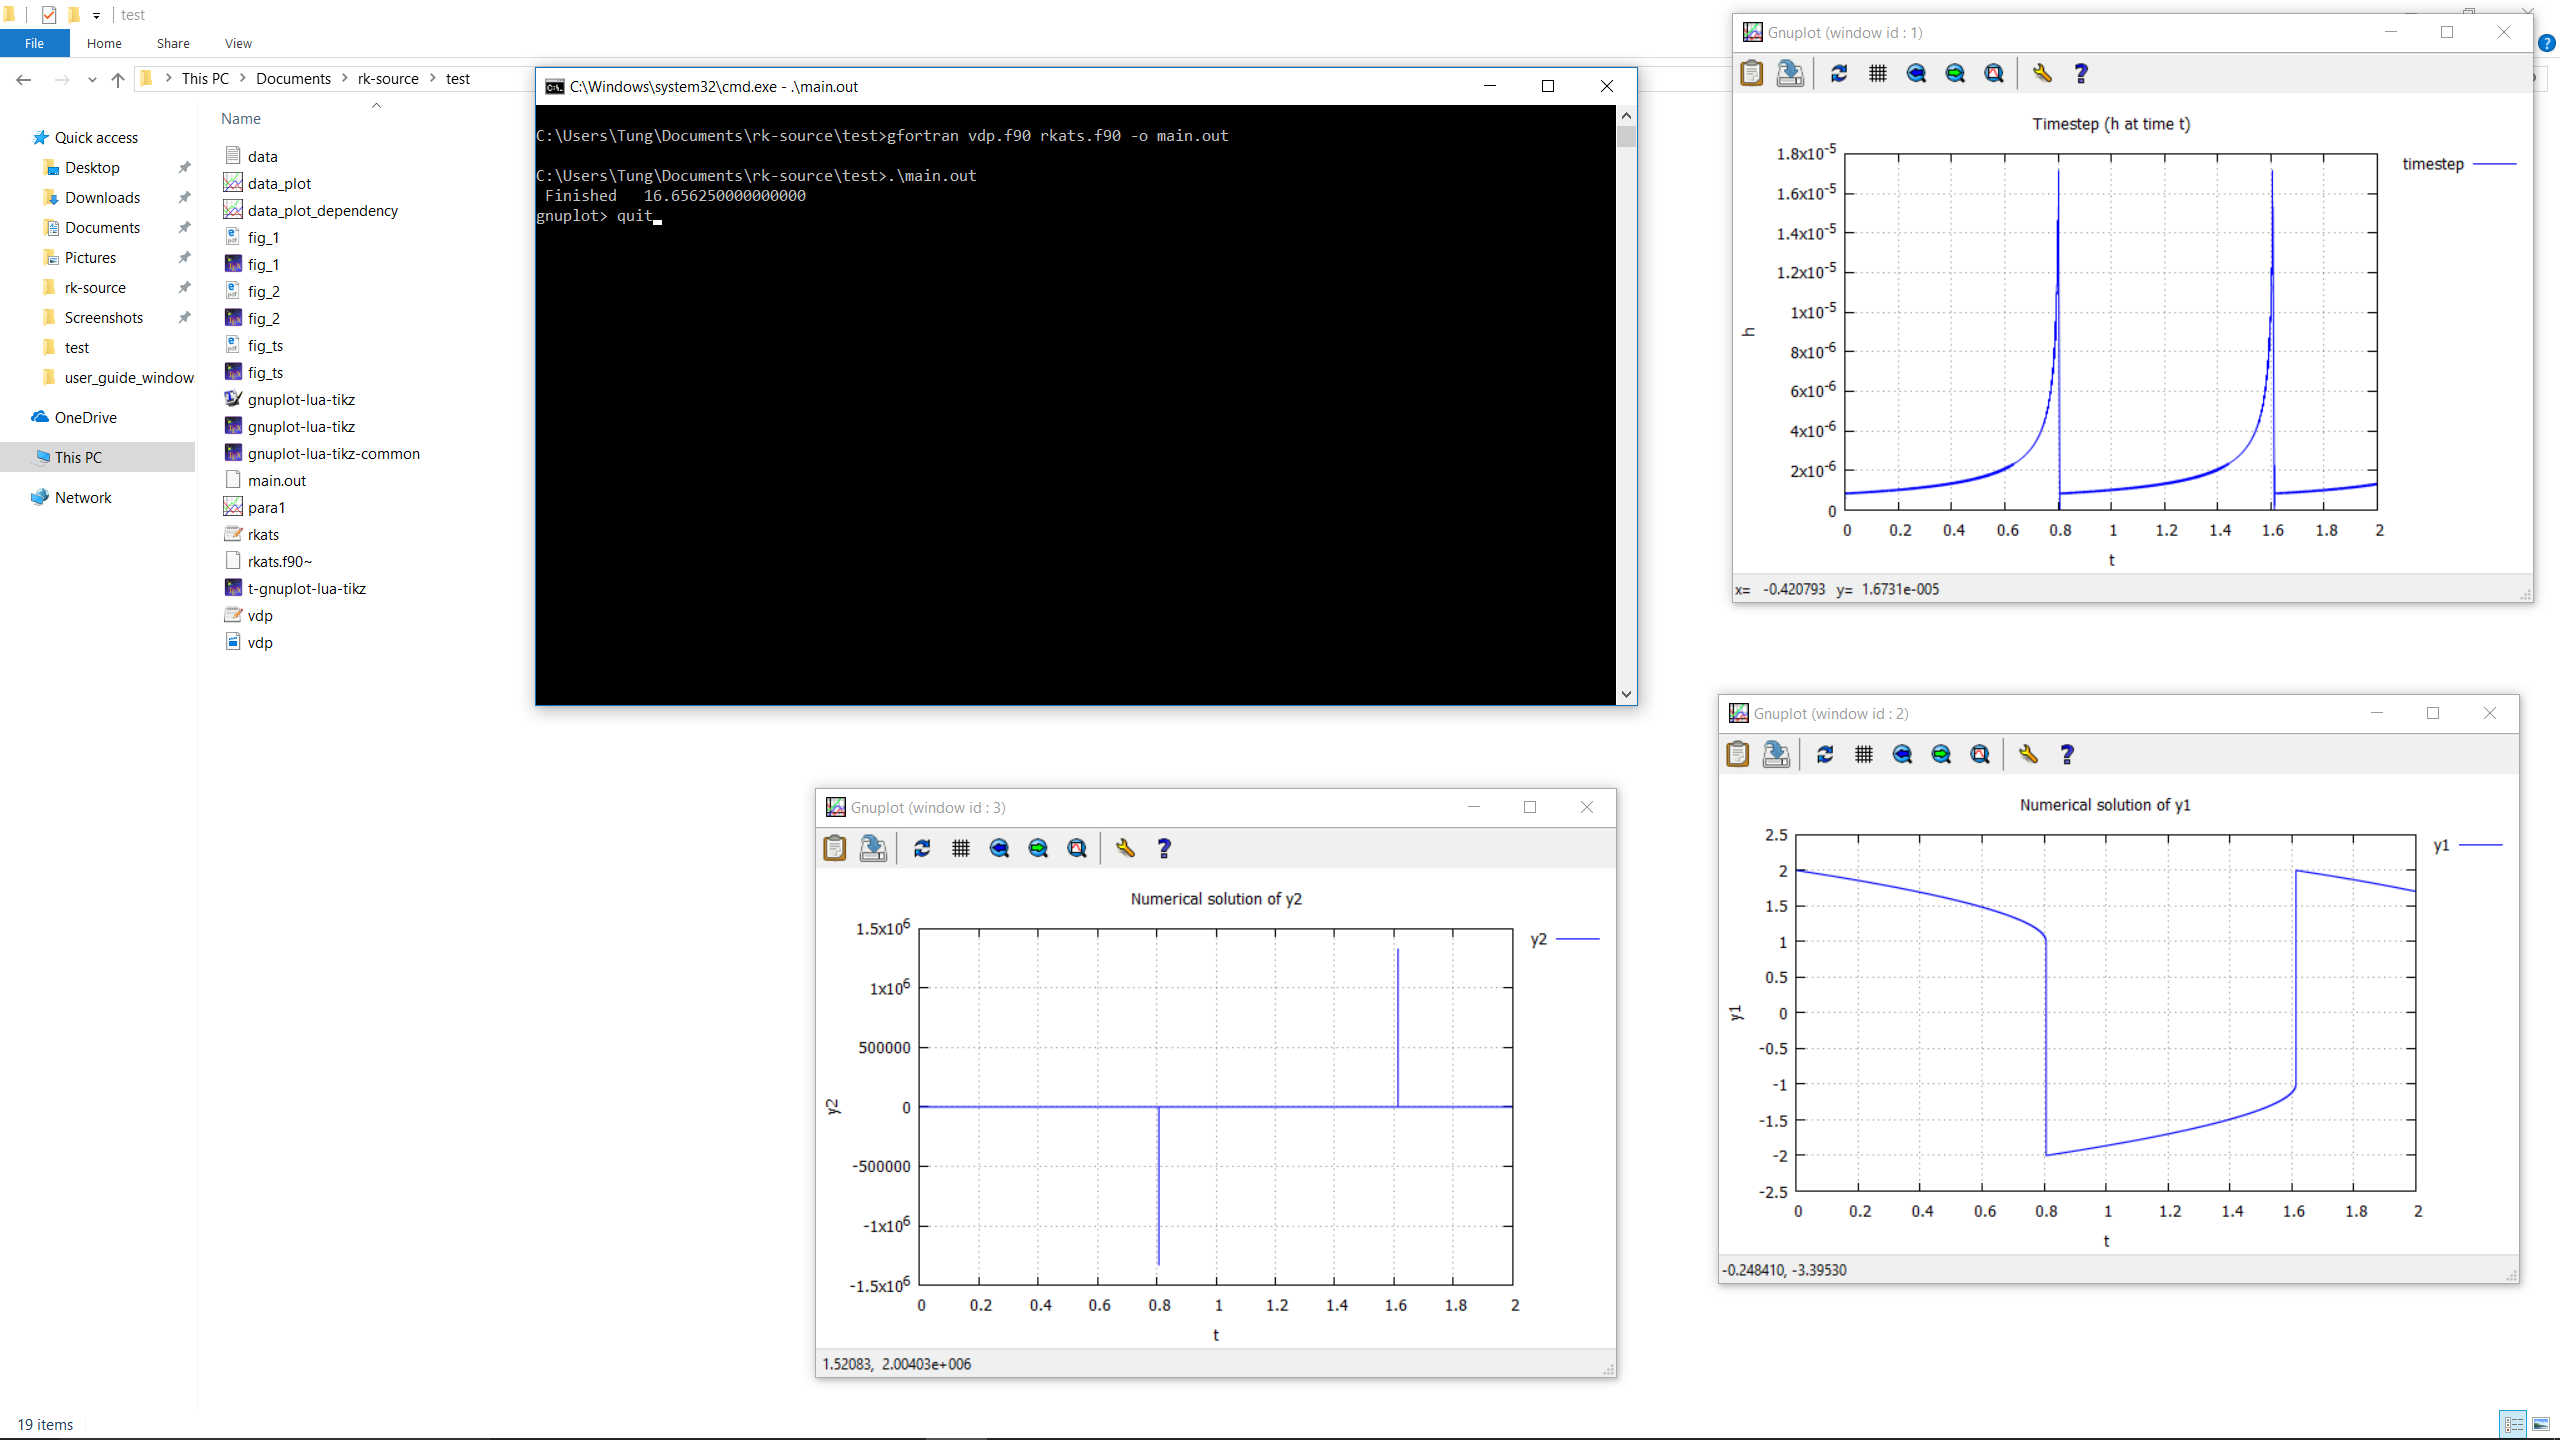
\includegraphics[width=15cm]{fig81}
		\caption{Typing the command in the Command Prompt}
	\end{figure}
	\begin{figure}[H]
		\centering	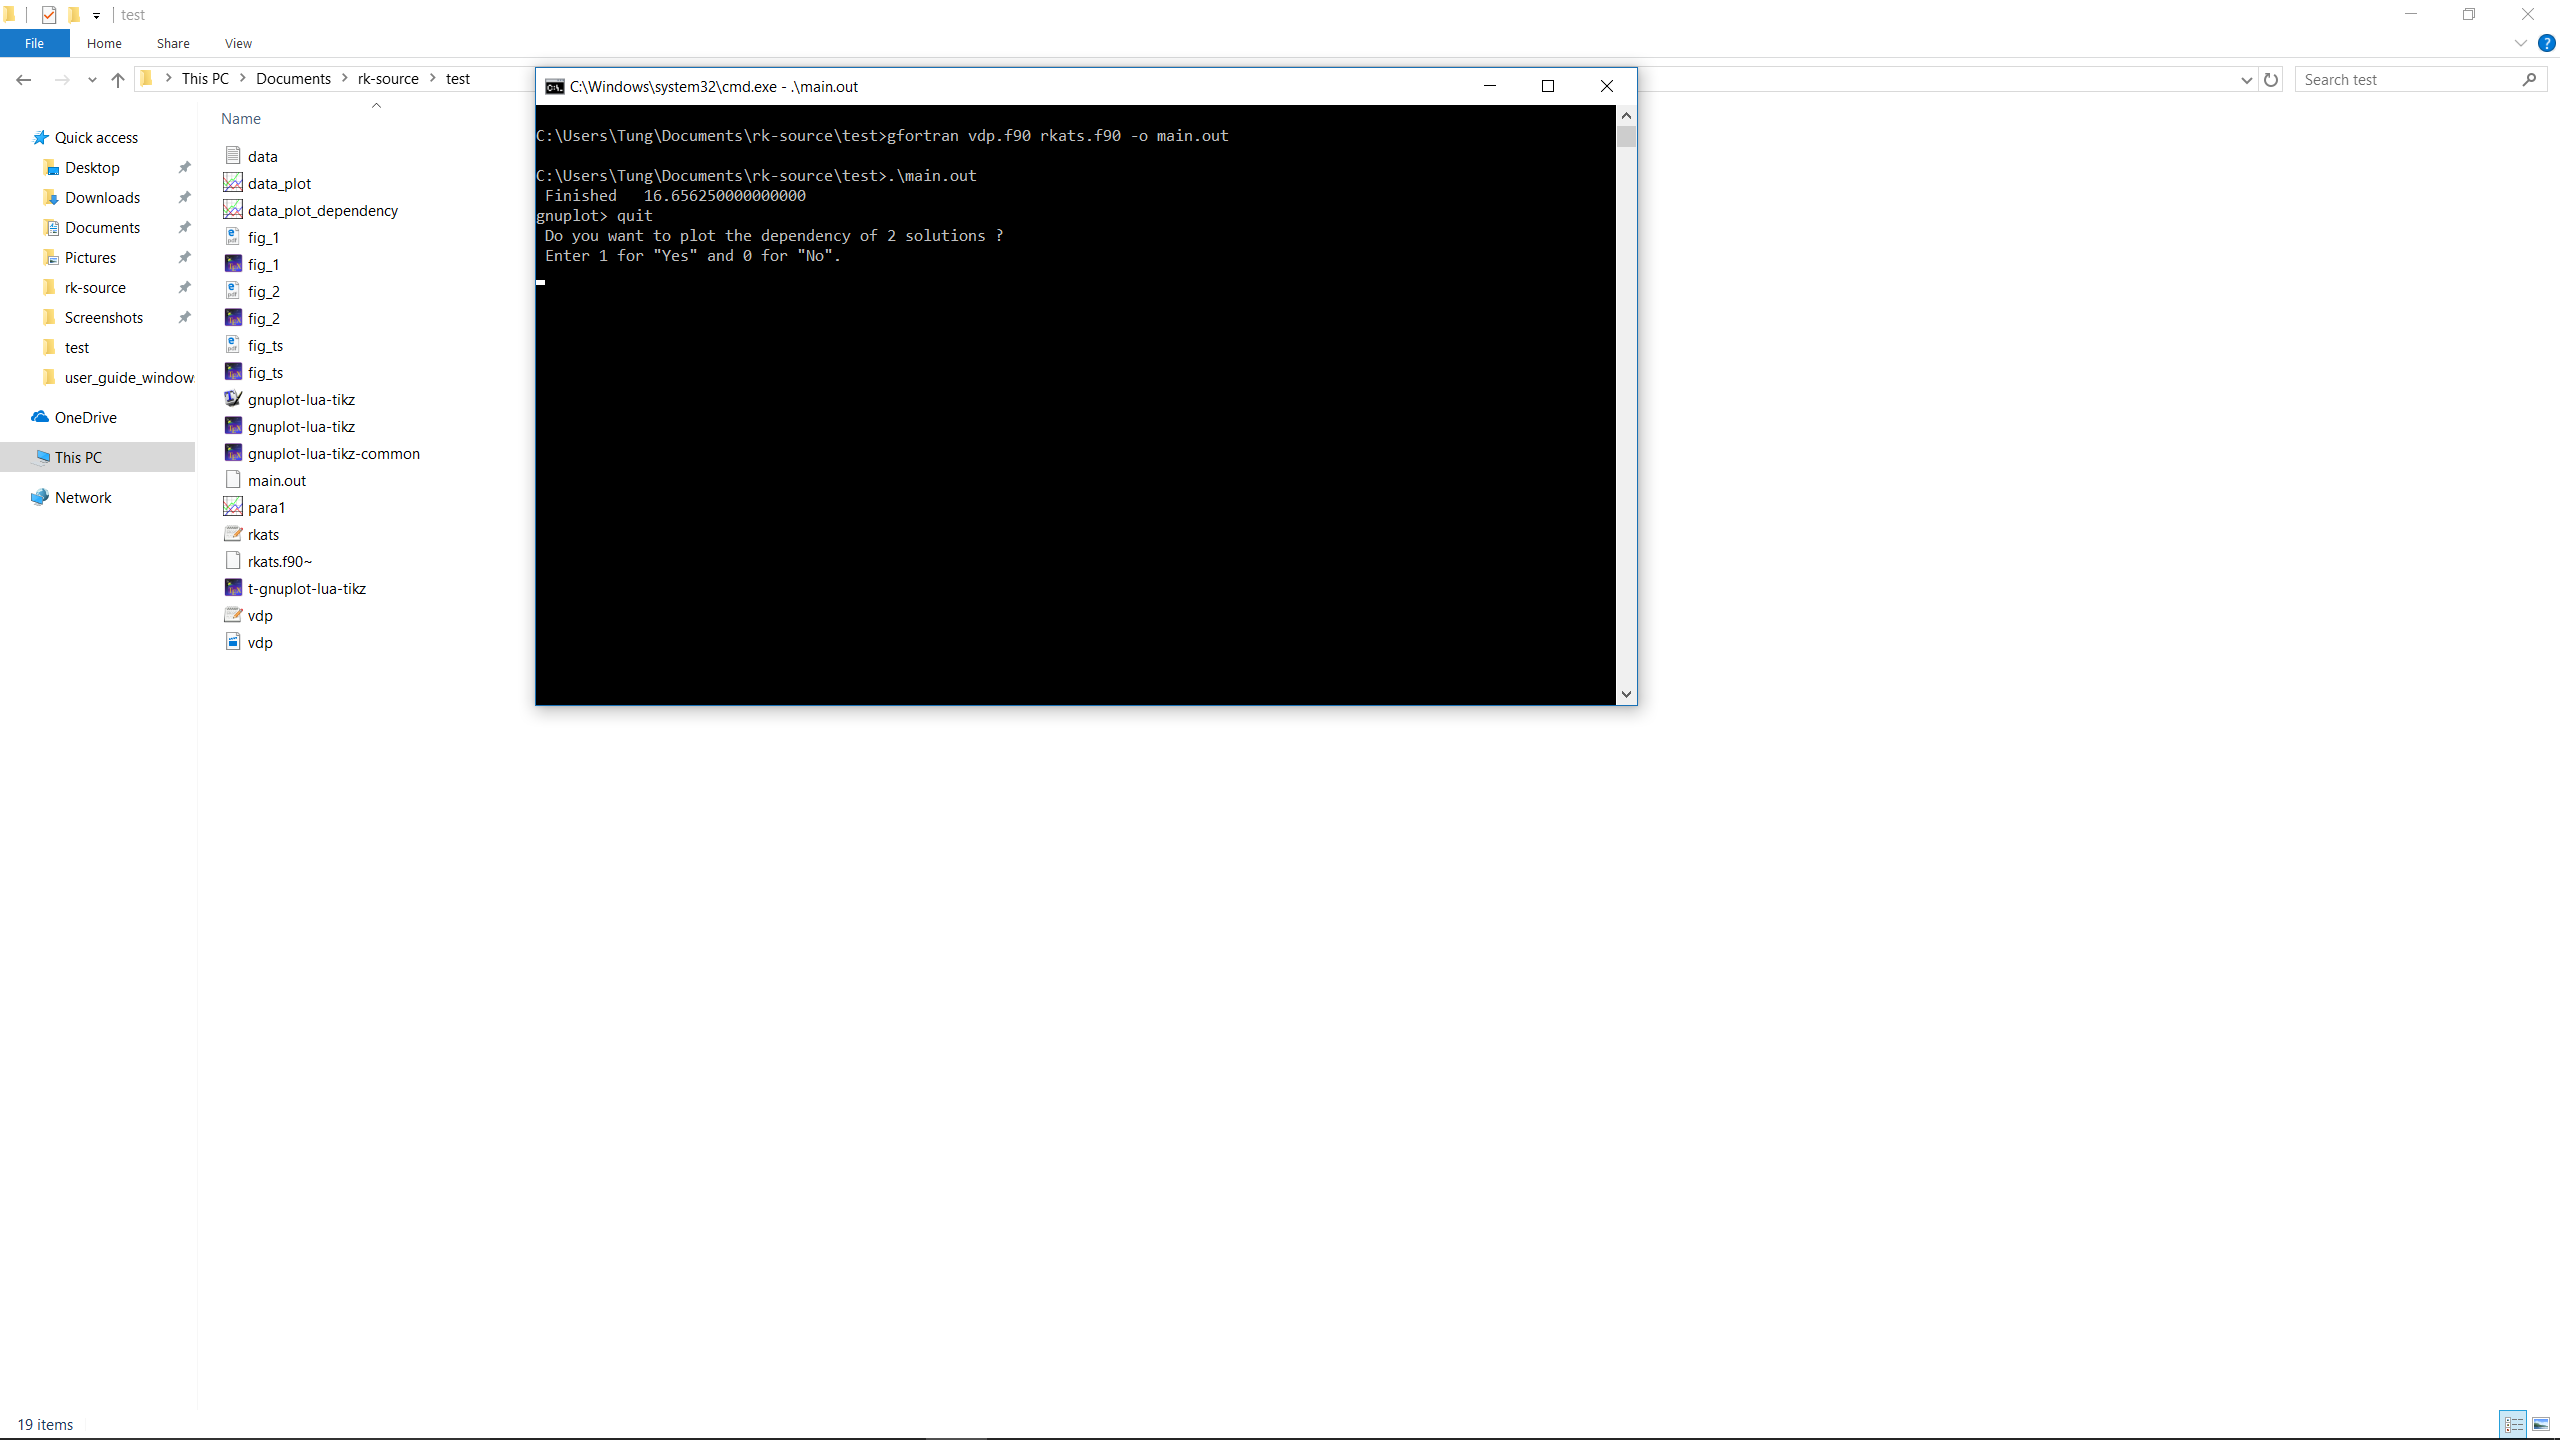
\includegraphics[width=15cm]{fig82}
		\caption{The result look like this}
	\end{figure}
	\noindent If the equation has more than one unknown variable (like in this example), the program will also ask whether if you want to plot the dependency between the solutions of those variables. This will be discussed in the next step.\\
	\noindent$\bullet$ \textbf{Step 6*:} Plot the dependency between the solutions of variables. To do this, you just need to follow the instructions in the \textbf{Command Prompt}. Suppose you want to plot the dependency of $y_1$ and $y_2$, type $1$ in the \textbf{Command Prompt} to confirm your intention, then type in $1$ and $2$ respectively for the next $2$ line.\\
	\begin{figure}[H]
		\centering	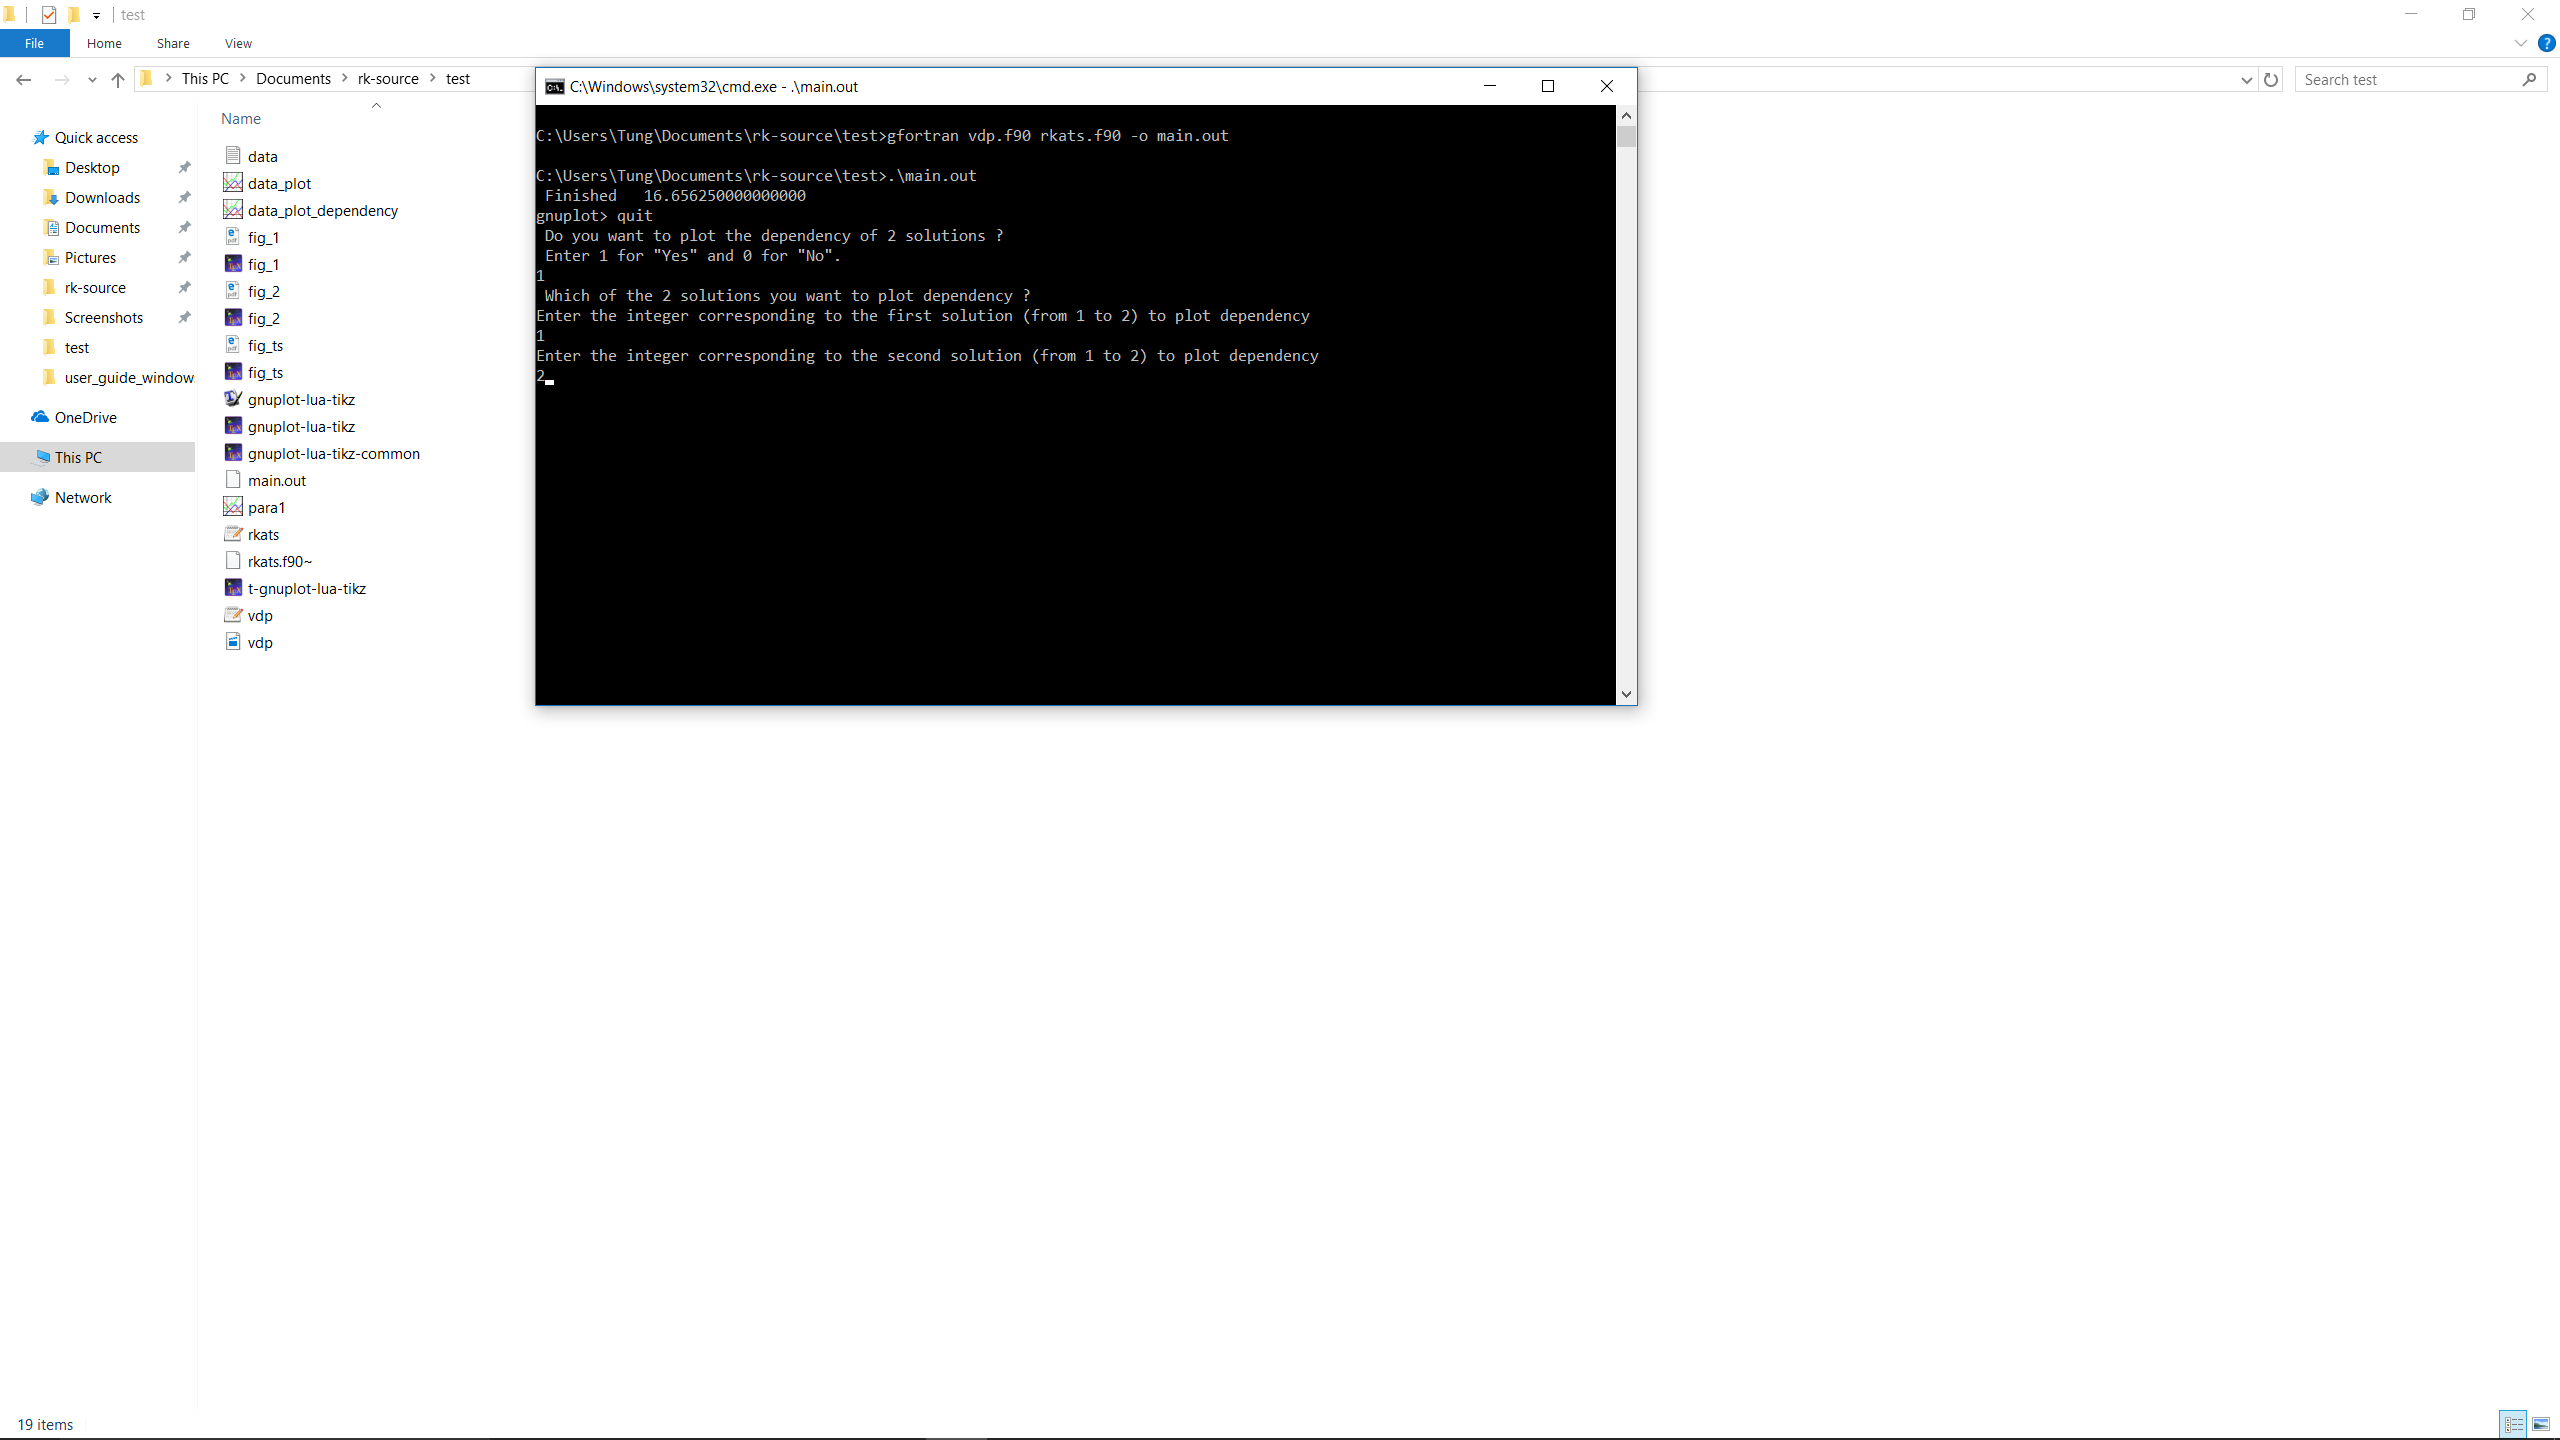
\includegraphics[width=15cm]{fig9}
		\caption{Typing the integers correspond to your choices in the Command Prompt}
	\end{figure}
	\noindent The result will be a new plot of the dependency, like before, additional files of the plot will appear.
	\begin{figure}[H]
		\centering	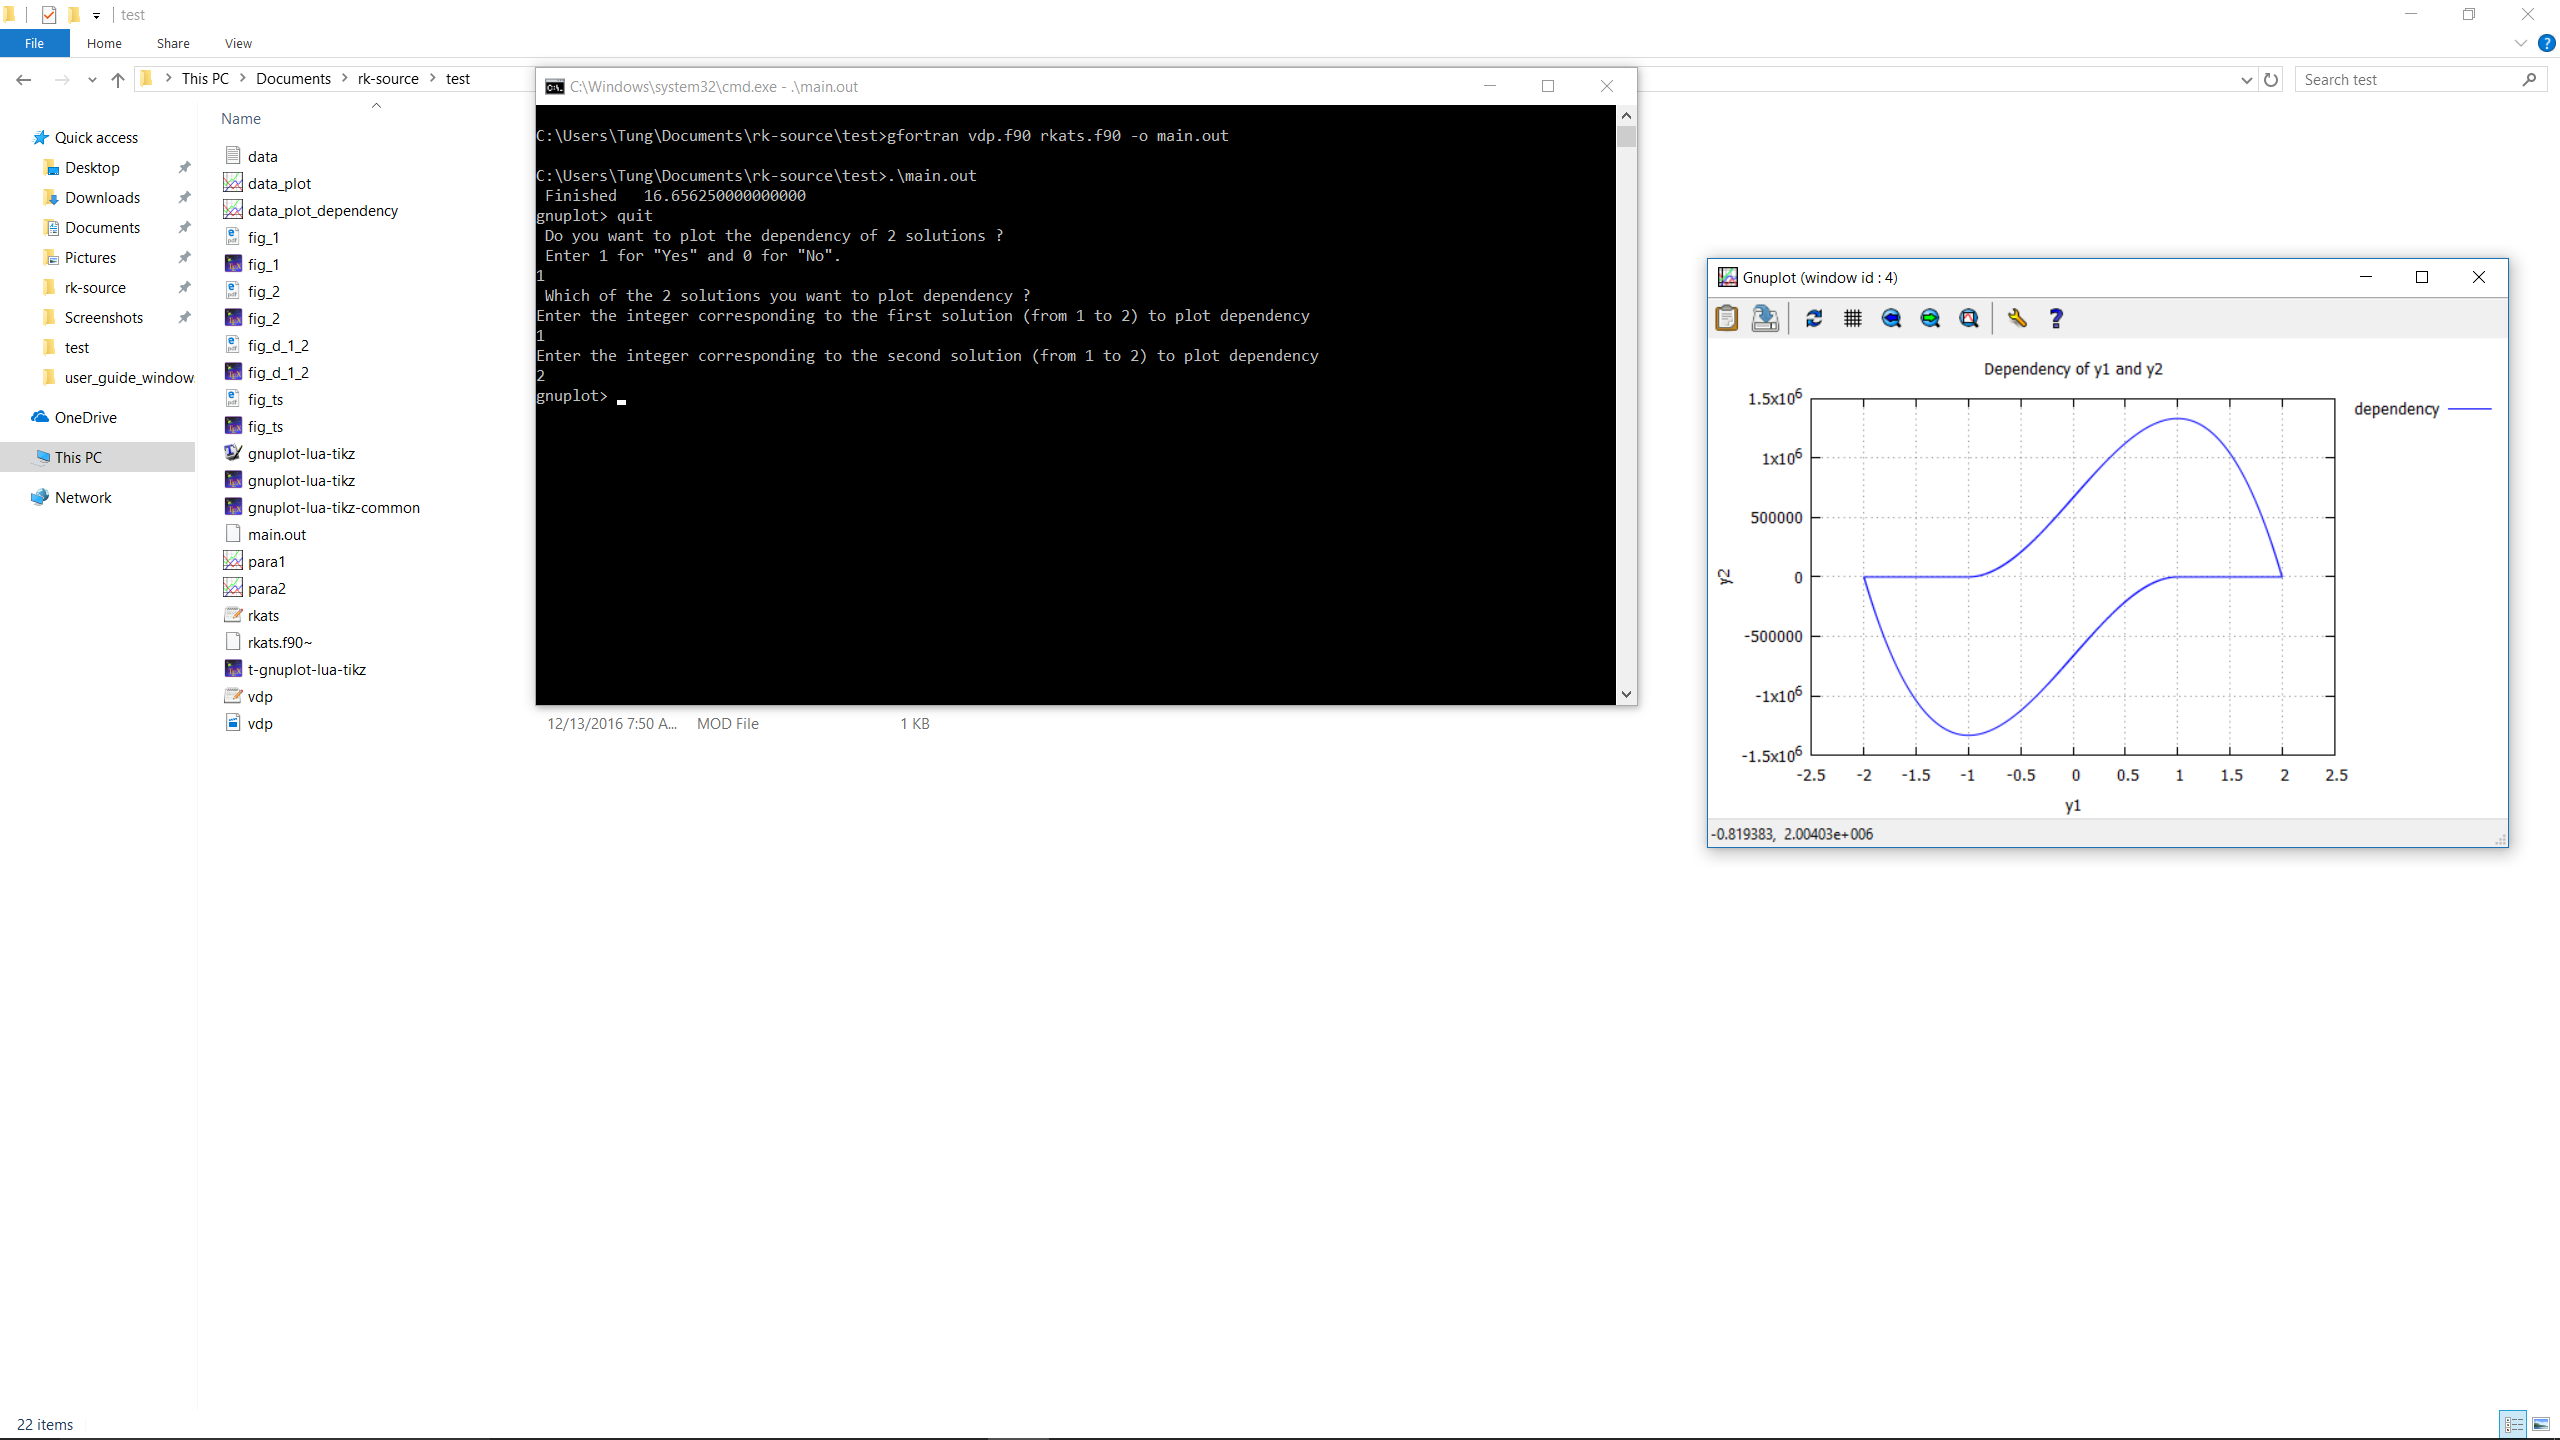
\includegraphics[width=15cm]{fig10}
		\caption{The result look like this}
	\end{figure}
	\noindent Similarly to above, to continue, type \texttt{quit} in the Command Prompt to quit the current \texttt{gnuplot} windows.
	\begin{figure}[H]
		\centering	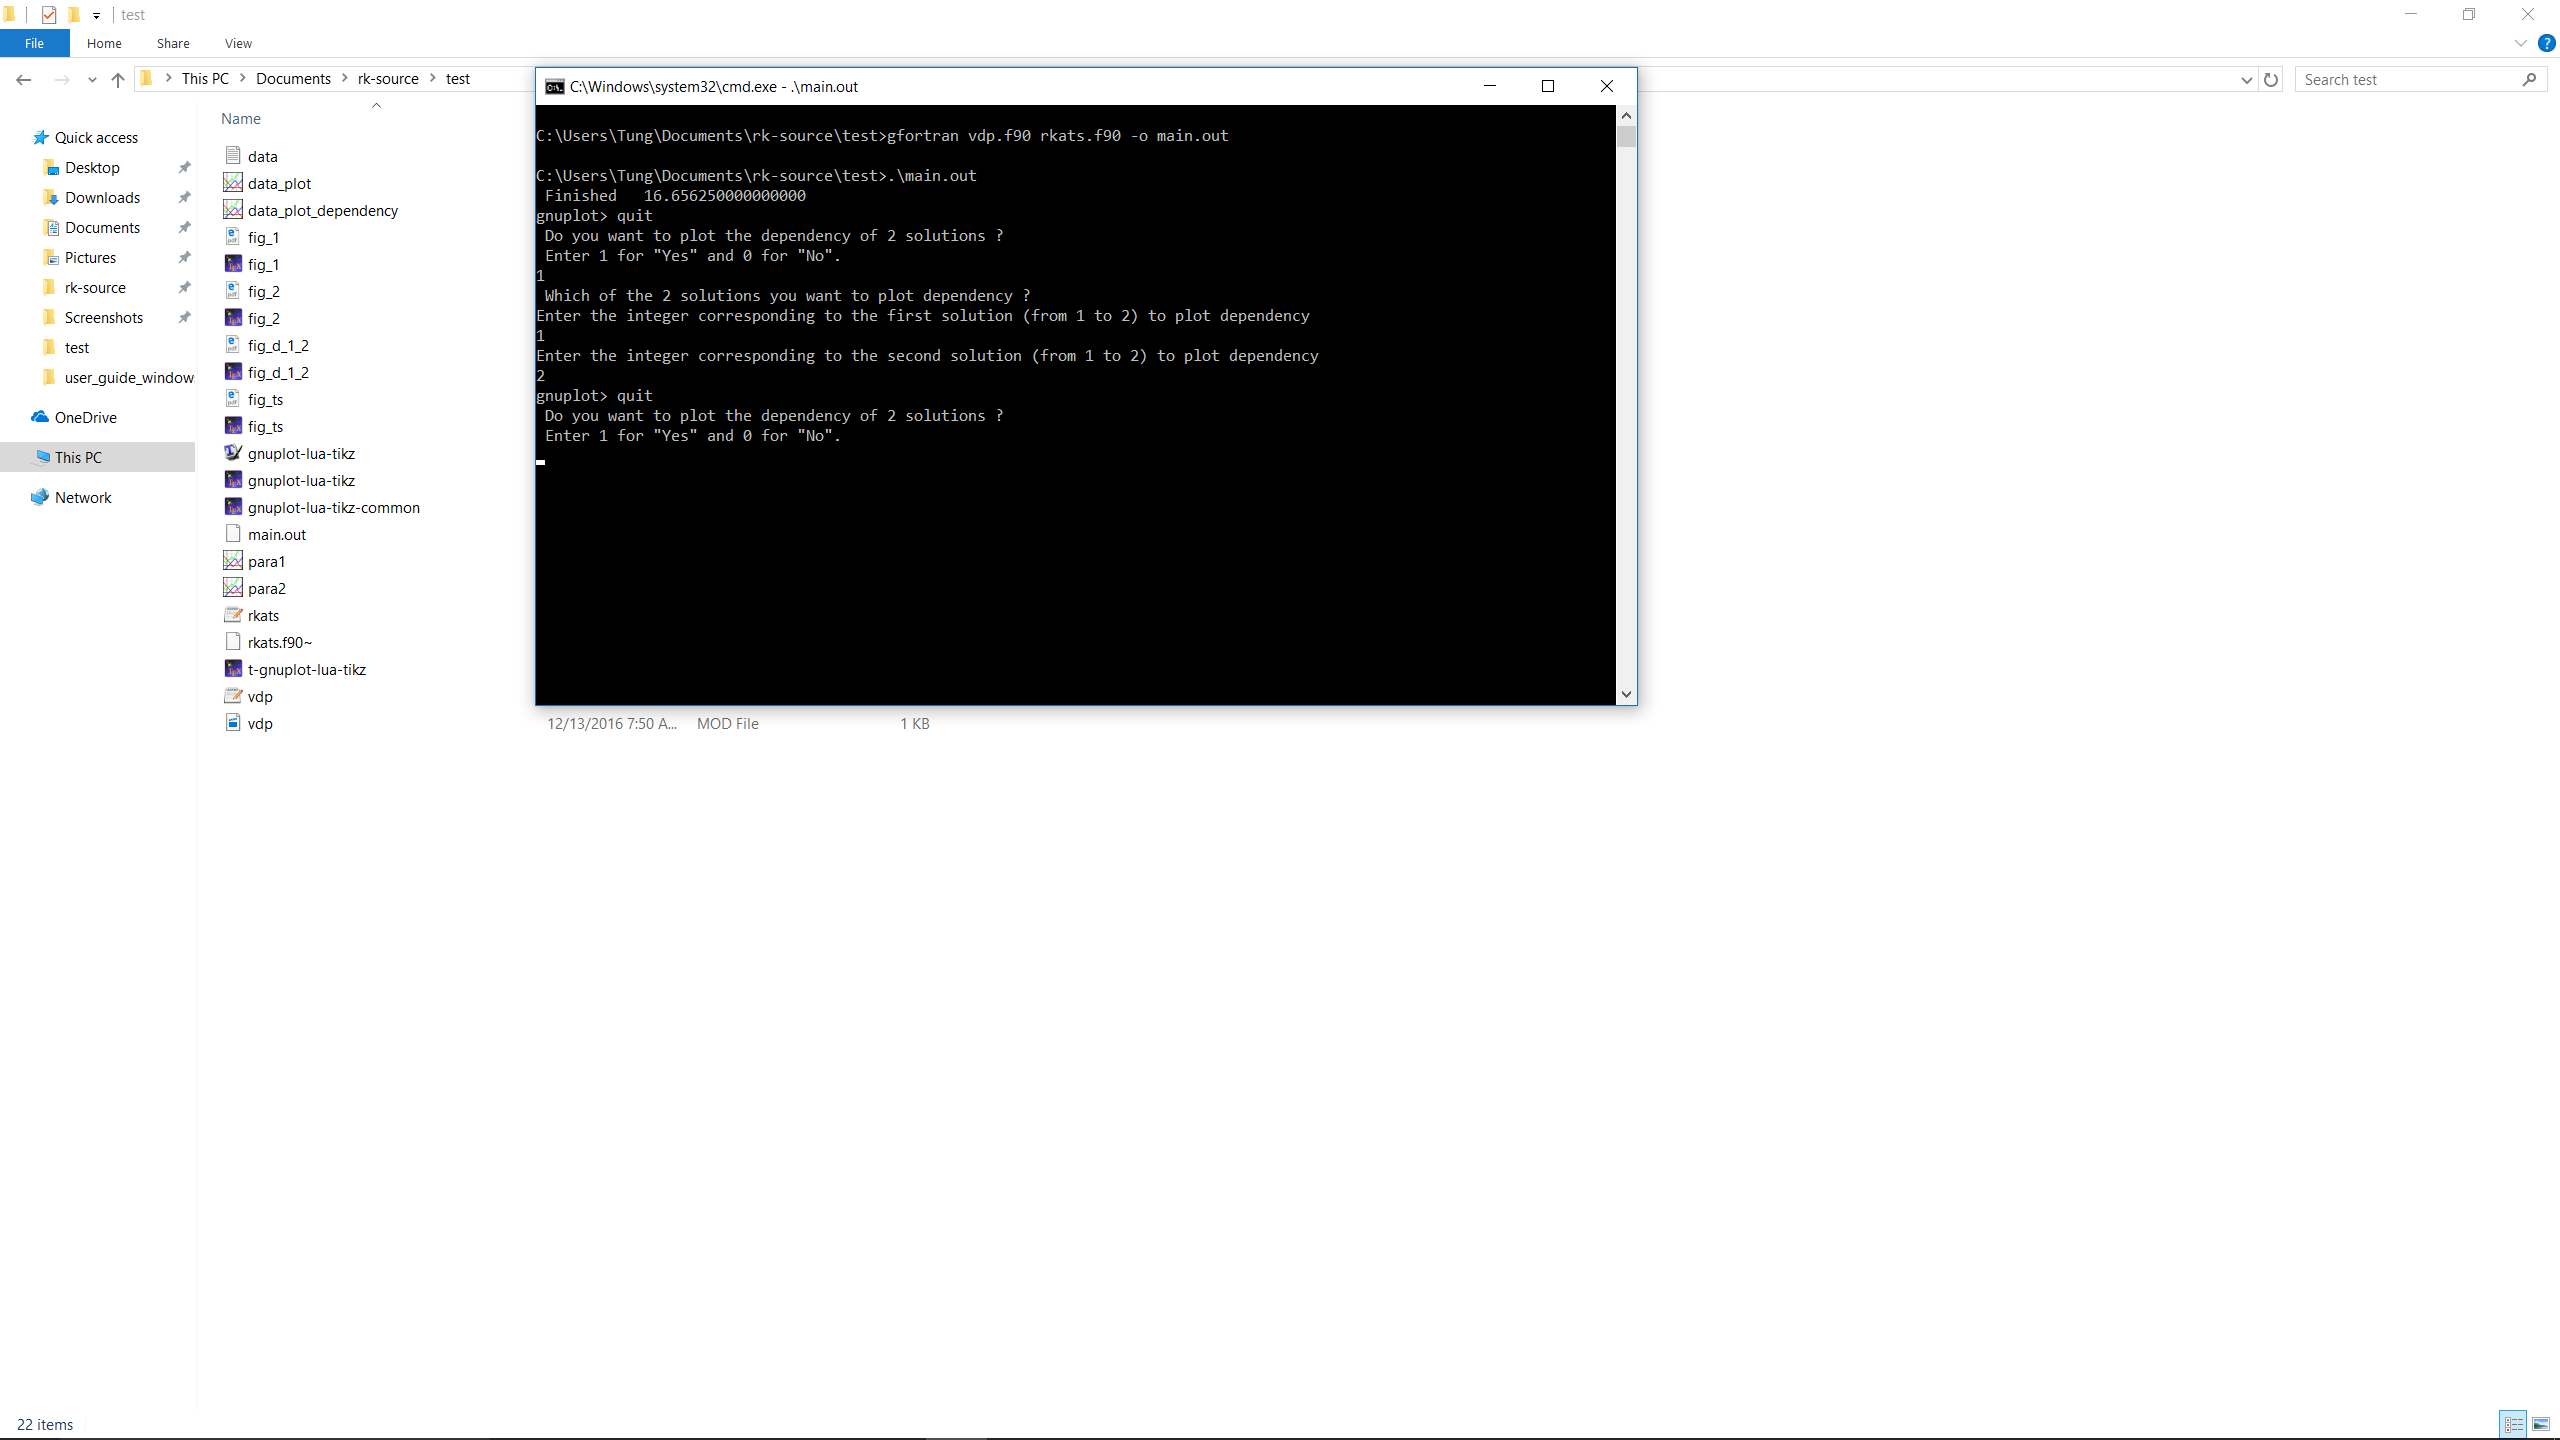
\includegraphics[width=15cm]{fig101}
		\caption{The result look like this}
	\end{figure}
	\noindent Now, if you want to continue plotting dependency (maybe if the equation you want to solve has more than $2$ variables), type $1$, or if you want to stop, type $0$.
	\begin{figure}[H]
		\centering	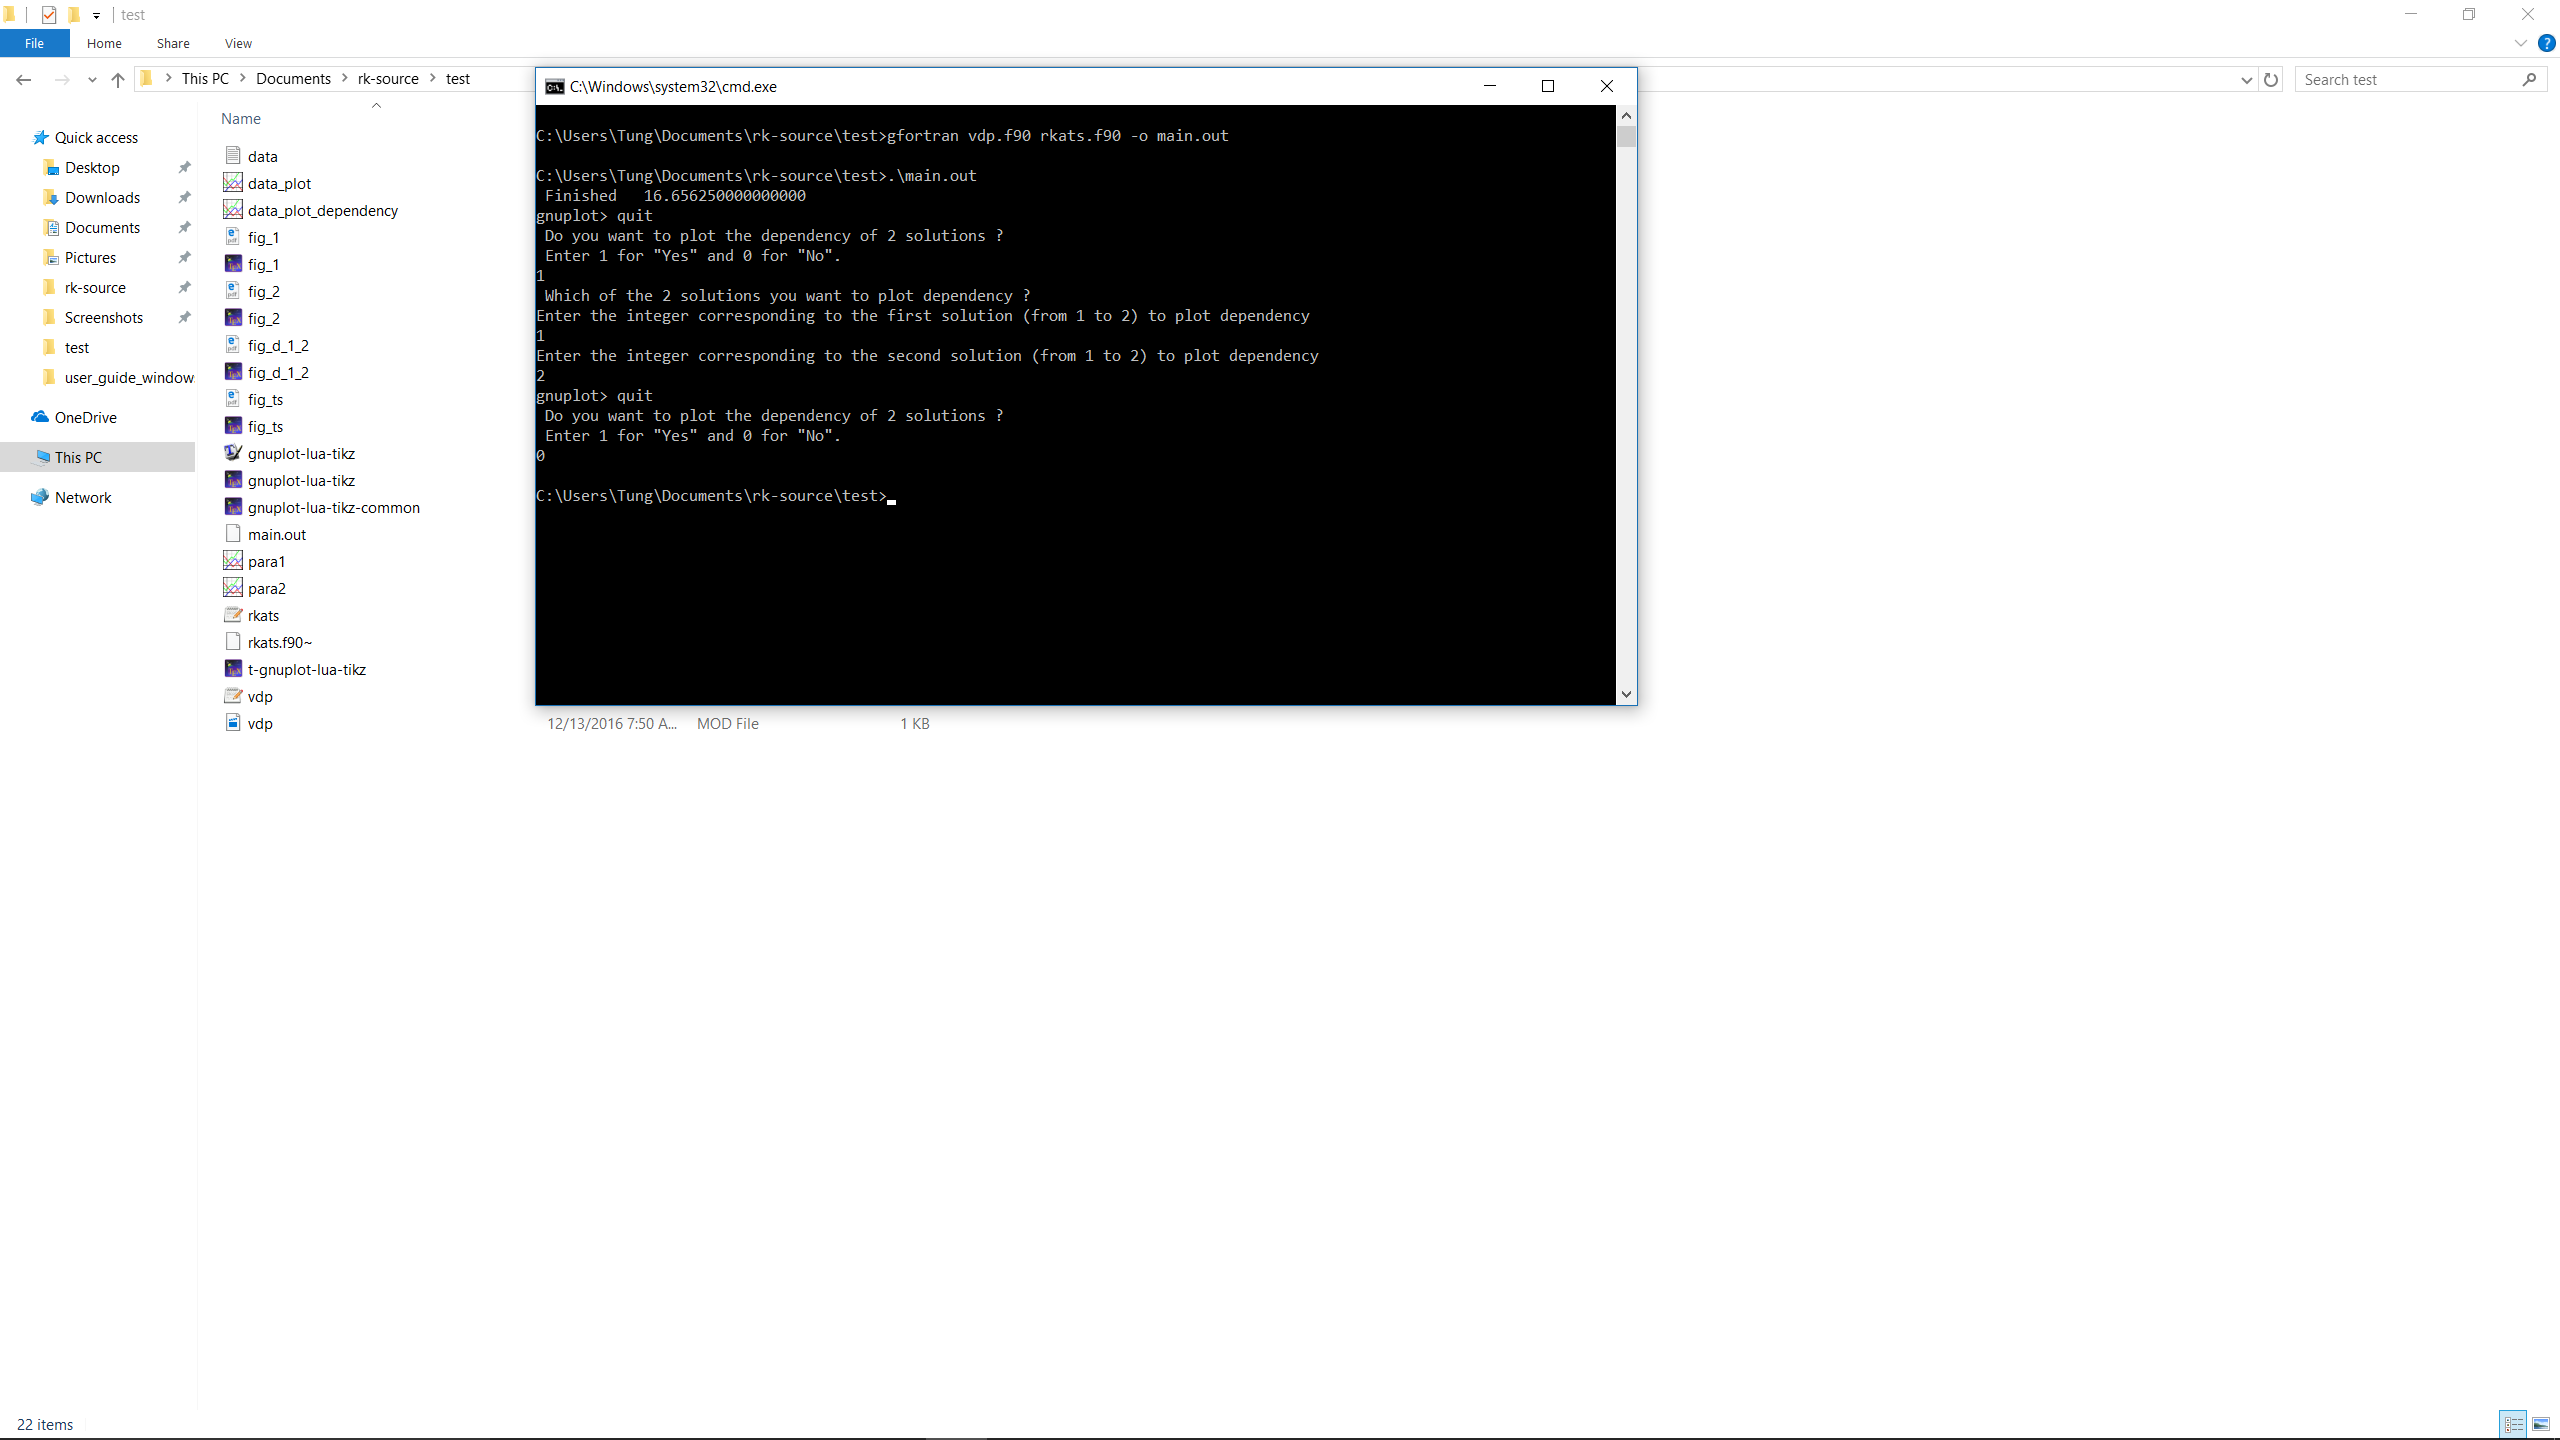
\includegraphics[width=15cm]{fig11}
		\caption{The program is stopped}
	\end{figure}
\newpage
\begin{thebibliography}{999}
	\bibitem {1} Tan Trung Nguyen, Frederique Laurent, Rodney Fox, Marc Massot. \textit{Solution of population balance equations in applications with fine particles: mathematical modeling and numerical schemes}. Journal of Computational Physics, Elsevier, 2016, 325
	\bibitem {2} Nguyen Quan Ba Hong, Doan Tran Nguyen Tung, Nguyen An Thinh, \textit{Runge Kutta Methods for Ordinary Differential Equations}, 2016.
	\bibitem {3} \url{http://fortranwiki.org/fortran/show/HomePage}
\end{thebibliography}
\end{document}
